% !TEX program = xelatex
% =====================================================================
%  arXiv:2112.12756v2 中译本 —— 主文件
%  原文：O. Chekeres, A. Losev, P. Mnev, D. R. Youmans,
%        "Two Field-Theoretic Viewpoints on the Fukaya-Morse A_inf Category"
%        arXiv:2112.12756v2 [hep-th], 10 Jul 2022, 27 pp.
%
%  编译：xelatex main.tex （建议跑两遍以生成目录与交叉引用）
%  依赖：ctex（中文字体）、amsmath, amssymb, amsthm, graphicx, geometry,
%        hyperref, verbatim, xcolor —— 均为 TeX Live / MiKTeX 标准宏包
%  图：figures/fig01.png … fig12.png（由原 PDF 矢量图按 400 dpi 裁剪）
%
%  编号约定：原文式号 (1)–(56)、定理 1、假设 2.2、例 1–7、注 2.1/3.1/3.2/4.1
%            全部原样保留（用 \tag 与 thmenv 环境手工落号），便于与原书对读。
% =====================================================================
\documentclass[11pt,a4paper,UTF8,fontset=windows]{ctexart}
% 非 Windows 平台请把 fontset=windows 换成 fontset=fandol 或 fontset=mac

% ---------- 译注体例开关（教授可一键关闭） ----------
\newif\ifshowtakeaway \showtakeawaytrue   % 各节“本节重点”
\newif\ifshownotes    \shownotestrue      % 批注附录（行内 % [Tutor Note: …] 只在源码中可见）

\usepackage{amsmath,amssymb,amsthm}
\usepackage[numbers,sort&compress]{natbib}  % \cite{fukaya,fukayaoh} -> [5,6]，与原文一致
\usepackage{graphicx}
\usepackage{verbatim}
\usepackage{xcolor}
\usepackage{geometry}
\geometry{left=2.55cm,right=2.55cm,top=2.4cm,bottom=2.4cm}
\usepackage[colorlinks=true,linkcolor=blue!45!black,citecolor=blue!45!black,
            urlcolor=blue!45!black,bookmarksnumbered=true]{hyperref}
\graphicspath{{figures/}}

\setcounter{tocdepth}{2}

% ---------- 排版微调：减少中英混排造成的 Overfull ----------
\setlength{\emergencystretch}{3em}
\tolerance=1500
\hbadness=10000

% ---------- 定理类环境：编号手写，照录原书 ----------
% 用法：\begin{thmenv}[可选标题]{类名}{原书编号} … \end{thmenv}
\newenvironment{thmenv}[3][]{%
  \par\addvspace{6pt}%
  \noindent\textbf{#2~#3.}%
  \if\relax\detokenize{#1}\relax\else\;{\itshape（#1）}\fi
  \quad\ignorespaces
}{\par\addvspace{6pt}}

% ---------- “本节重点”环境 ----------
\ifshowtakeaway
  \newenvironment{takeaway}{%
    \par\addvspace{10pt}%
    \noindent\rule{\linewidth}{0.6pt}\par\nobreak\addvspace{3pt}%
    \noindent\textbf{本节重点}\par\nobreak\addvspace{2pt}%
    \begingroup\small\noindent\ignorespaces
  }{%
    \par\endgroup\addvspace{3pt}%
    \noindent\rule{\linewidth}{0.6pt}\par\addvspace{10pt}%
  }
\else
  \excludecomment{takeaway}
\fi

\newcommand{\Ainf}{A_\infty}
\newcommand{\Mor}{\operatorname{Mor}}

\title{论 Fukaya--Morse $\Ainf$ 范畴的两种场论视角}
\author{O.~Chekeres,\ A.~Losev,\ P.~Mnev,\ D.~R.~Youmans}
\date{arXiv:2112.12756v2 [hep-th]，2022 年 7 月 10 日}

\begin{document}

\begin{center}
  {\LARGE\bfseries 论 Fukaya--Morse $\Ainf$ 范畴的两种场论视角}\\[8pt]
  {\large Two Field-Theoretic Viewpoints on the\\ Fukaya--Morse $\Ainf$ Category}\\[12pt]
  {\large O.~Chekeres\quad A.~Losev\quad P.~Mnev\quad D.~R.~Youmans}\\[6pt]
  {\small arXiv:2112.12756v2 [hep-th]\quad 2022 年 7 月 10 日\quad 原文 27 页}
\end{center}

\vspace{0.5em}
\noindent\textbf{摘要.}\quad
本文研究 Fukaya $\Ainf$ 范畴的 Morse 退化的一种增强版本，其高阶复合由梯度流树的数目给出。所谓“增强”，是指允许一个对象到自身的态射取为该流形上的链。高阶复合对应于对经过给定一族链的 Morse 树作计数。对于这一构造以及复合映射的 $\Ainf$ 关系式的两种证明，我们给出两种视角。一种视角来自在特殊规范下计算出的 BF 理论的有效作用量；另一种视角来自高阶拓扑量子力学。

\vspace{0.6em}
\noindent\textbf{关键词：}\ $\Ainf$ 范畴；Fukaya--Morse 范畴；Morse 树；BF 理论；Batalin--Vilkovisky 形式；拓扑量子力学

\vspace{0.4em}
\noindent\textbf{原文 MSC 分类：}\ 53D37, 53D40, 81T45（据原文主题归类补注，仅供检索）

\medskip
\noindent\rule{\linewidth}{0.4pt}

% =====================================================================
%  译校说明
% =====================================================================
\section*{译校说明}
\addcontentsline{toc}{section}{译校说明}

\begin{enumerate}
  \item \textbf{底本。}译文以 arXiv:2112.12756v2（2022-07-10，27 页）为准，未参考其它版本。文中所标“原书 p.$N$”均指该 PDF 页码，arXiv 版正文与页码一一对应，无需偏移。
  \item \textbf{编号一律照录。}原文的式号 (1)--(56)、定理 1、假设 2.2、例 1--7、注 2.1/3.1/3.2/4.1、图 1--12 全部保持原编号，源码中以 \verb|\tag{…}| 与 \verb|thmenv| 环境手工落号。这样读者可直接拿中译与原 PDF 对读，批注中的定位也才有意义。
  \item \textbf{术语。}以中文学界通行译名为准（如 gauge theory 规范场论、holonomy 和乐群、anomaly 反常；本文涉及 $A_\infty$ 范畴、BV 形式、有效作用量、横截性等）。保留英文的术语（\verb|Lefschetz thimble|、Fukaya、Morse--Smale、Feynman 图等）在首次出现处给括注，此后一律英文。全书术语冻结表见 \verb|work/glossary.md|。
  \item \textbf{批注。}源码中形如 \verb|% [Tutor Note: …]| 的行为译校批注，只写在源码里、不进入排版结果，共三类：易错预警（符号、指标、次数、约定）、含糊点拨（作者以“显然”跳过的论证，点出所用定理与可查文献）、背景直觉。全部批注另按节汇总于附录~\ref{app:notes}，可用导言区开关 \verb|\shownotestrue|／\verb|\shownotesfalse| 整体显示或隐藏。
  \item \textbf{本节重点。}每节开头给出“本节重点”，提炼物理图像、数学工具与主要结论，可用 \verb|\showtakeawayfalse| 关闭。
  \item \textbf{不擅改原文。}原文的笔误、含糊与省略一律保留，只在同处加批注并在附录中登记；译文不补写原文没有的内容。
  \item \textbf{编译。}\verb|xelatex main.tex| 两遍；中文由 \verb|ctex| 宏包处理（Windows 下自动使用宋体/黑体，非 Windows 平台请改 \verb|fontset|）。图表文件在 \verb|figures/| 目录。
\end{enumerate}

\medskip
\noindent\rule{\linewidth}{0.4pt}

\tableofcontents
\newpage

% =====================================================================
%  正文
% =====================================================================
% =====================================================================
%  第 1 节  引言（原书 p.2–3）
% =====================================================================
\section{引言}\label{sec:1}

% [Tutor Note: 本节是全文的路标，一句话概括：把 Fukaya 范畴在余切丛 $T^*X$ 上取半经典极限 $\epsilon\to0$，全纯圆盘的计数就退化为梯度流树的计数；本文补上“对象到自身”的态射，并给出 $A_\infty$ 关系式的两个非全纯证明。]

\begin{takeaway}
\begin{itemize}
  \item \textbf{物理图像}：Fukaya 范畴用全纯圆盘的计数定义 Lagrange 子流形之间的高阶复合。在余切丛 $T^*X$ 上取 $L_a=\mathrm{graph}(\epsilon\,\mathrm{d}F_a)$ 并令 $\epsilon\to0$，全纯圆盘投影到 $X$ 后收缩为梯度流树，全纯计数因而退化为 Morse 理论中的计数。此即 Fukaya--Morse $\Ainf$ 范畴。
  \item \textbf{数学工具}：$\Ainf$ 预范畴、Morse 链复形、生成函数、带状树、横截性。
  \item \textbf{主要结论}：该构造原本缺“对象到自身的态射”。本文取 $\Mor(F_a,F_a)=C^{\mathrm{sing}}_\bullet(X;\mathbb Z)$ 补上这一环，得到增强的 Fukaya--Morse $\Ainf$ 范畴，并给出 $\Ainf$ 关系式的两种证明：BF 理论的有效作用量（二次量子化）与度量树上的高阶拓扑量子力学（一次量子化）。两个证明都不使用全纯圆盘。
\end{itemize}
\end{takeaway}

Fukaya 在 \cite{fukaya} 中引入了一个 $\Ainf$ 范畴：对象是辛流形中的 Lagrange 子流形，态射是这些子流形交点的形式线性组合，高阶复合则以这些子流形为边界的全纯圆盘\footnote{这里沿用一个习惯的术语滥用：下文说“全纯”，指的其实是“伪全纯”，即相对于辛流形上一个相容的殆复结构而言。}的计数来定义。\footnote{细节参看 \cite{fukayaoh,seidel}；本主题的入门导引见 \cite{auroux}。}若辛流形是余切丛 $T^*X$，且 Lagrange 子流形都能投影到底流形 $X$ 上，则 $N$ 个不同的 Lagrange 子流形 $L_a$（假定它们都是正合的）可用 $N$ 个生成函数 $F_a$ 来描述，$L_a$ 由方程
\begin{equation*}
  p_i=\frac{\partial F_a}{\partial X^i}
\end{equation*}
给出，其中 $p_i$ 是与底流形坐标 $X^i$ 对偶的纤维坐标。于是 Lagrange 子流形的交点投影为生成函数之差的临界点 $P_{\alpha,ab}$：
\begin{equation*}
  \mathrm{d}(F_a-F_b)=0.
\end{equation*}
若作重标度 $F_a\to\epsilon F_a$，则全纯圆盘到底流形的投影趋于由生成函数之差的梯度轨道拼成的带状树。计数这类带状树就确定了某个 $\Ainf$ 范畴的复合映射。为与辛流形中由全纯圆盘计数给出的“通常的”Fukaya 范畴相区别，我们称这一结构为“Fukaya--Morse $\Ainf$ 范畴”。细节见原始论文 \cite{fukaya,fukayaoh}，以及 \cite{kontsevichsoibelman}。

% [Tutor Note: “重标度 $F_a\to\epsilon F_a$”是全篇第一个易错点：$\epsilon\to0$ 时 $L_a=\mathrm{graph}(\epsilon\,\mathrm{d}F_a)$ 退化到零截面，交点 $P_{\alpha,ab}$ 趋于 $\mathrm{d}(F_a-F_b)=0$ 的临界点，全纯圆盘的半径随之趋于零。作者在此省略了“一列全纯圆盘收敛到梯度流树”的紧性论证，标准做法是用 Gromov 紧性与 $T^*X$ 上近全纯曲线的局部描述，见 Fukaya--Oh \cite{fukayaoh} 与 Seidel \cite{seidel} 第 9 章。]

这一构造所缺的，是对象到自身态射的描述。我们想补上这一空缺，给出一个包含这类态射的 $\Ainf$ 结构。本文将给出构造，并给出 $\Ainf$ 关系式的两个不同证明。两个证明都不涉及全纯圆盘。

% [Tutor Note: “两个证明都不涉及全纯圆盘”是全文纲领，值得停一下。其一只用 BV 形式的纤维积分与树形求和（等价于 Kontsevich--Soibelman 同伦转移定理，见 \cite{kontsevichsoibelman}）；其二只用度量树模空间上一个闭微分形式与 Stokes 定理。换言之，作者把“辛几何”这一层完全剥离，只留下“生成函数之差是 Morse--Smale 函数”与“梯度流”两件事。这也解释了为什么证明能同时给出整系数版本与一般的环系数版本。]

\subsection{结果概述}\label{sec:1.1}

\begin{takeaway}
\begin{itemize}
  \item \textbf{物理图像}：三点新意分别对应“补上自同态”（第~\ref{sec:2} 节）、“把整个结构翻译成 BF 理论的有效作用量”（第~\ref{sec:3} 节）、“把同一批数据翻译成树上的高阶拓扑量子力学”（第~\ref{sec:4} 节）。
  \item \textbf{数学工具}：奇异链与余维数分次、Batalin--Vilkovisky（BV）主方程、模空间上的积分与周期的 Stokes 定理。
  \item \textbf{主要结论}：$\Ainf$ 关系式在这里可看作 BV 主方程在“慢场”上的投影，也可看作“度量树模空间上闭形式在边界处分解”的 Stokes 推论。
\end{itemize}
\end{takeaway}

与已有文献相比，本文的新意有以下三点。

\begin{enumerate}
  \item[(A)] \textbf{第~\ref{sec:2} 节}：用一个对象自同态的模型来增强 Fukaya--Morse $\Ainf$ 范畴，即取
  \begin{equation*}
    \Mor(F_a,F_a)=C^{\mathrm{sing}}_\bullet(X,\mathbb Z),
  \end{equation*}
  也就是 $X$ 上的奇异链。高阶复合由一个计数几何问题定义：在 $X$ 中计数由梯度轨道构成的树，这些树连接给定的一组临界点，并经过给定的一组链。
  \item[(B)] \textbf{第~\ref{sec:3} 节}：用拓扑规范理论（BF 理论）在特定规范下算出的有效作用量，来描述增强 Fukaya--Morse $\Ainf$ 范畴的数据。在此框架中，$\Ainf$ 范畴的结构关系式由有效作用量的 Batalin--Vilkovisky 主方程推出。
  \item[(C)] \textbf{第~\ref{sec:4} 节}：用高阶拓扑量子力学来描述同一批数据，即给出度量树模空间上的一个微分形式 $I$。用这套语言，$\Ainf$ 复合映射是形式 $I$ 的周期，$\Ainf$ 关系式则由模空间上的 Stokes 定理与 $I$ 在模空间边界处的分解性质推出。此证明是上同调场论中 WDVV 方程证明的一维类比，见 \cite{kontsevichmanin}。
\end{enumerate}

% [Tutor Note: (B) 的逻辑方向容易说反。BV 主方程 $\{S_{\mathrm{eff}},S_{\mathrm{eff}}\}=0$ 直接给出的是 $L_\infty$ 关系式（斜对称化之后的结果）；要得到 $A_\infty$ 关系式，必须把系数代数换成上三角矩阵代数 $\mathcal A$ 再张量，见注 3.2 与式 (47)。作者在 (B) 里没有点破这一层，读者若不留意会误以为 $A_\infty$ 关系式可以直接从 BV 主方程读出。]

% [Tutor Note: (A) 中“取奇异链”不是任意选择：$F_a-F_a\equiv0$ 的临界点集是整个 $X$，故自同态的 Morse 复数形式上就是 $X$ 上的链；取奇异链（而非只取点）使复合映射 (4) 能作用在“被看作分布”的链上。若改取 de Rham 形式或上链，会付出别的代价，见第 2.7 节与我在此处的批注。]
\endinput

% =====================================================================
%  第 2 节（开头）与 2.1 节  增强的 Fukaya–Morse A∞ 范畴：定义（原书 p.3–5）
% =====================================================================
\section{增强的 Fukaya--Morse $\Ainf$ 范畴：构造与例子}\label{sec:2}

\begin{takeaway}
\begin{itemize}
  \item \textbf{物理图像}：把“对象到自身”的态射也算进来。$F_a$ 到 $F_b$（$a\neq b$）的态射是 Morse 链，$F_a$ 到自身的态射取为 $X$ 上的奇异链；高阶复合则数“经过给定一族链的 Morse 树”。
  \item \textbf{数学工具}：Morse 复形与余指标分级、奇异链复形及其余维数分级、Morse 树的模空间、横截性假设、循环 $\Ainf$ 复合。
  \item \textbf{主要结论}：得到的是一个\emph{部分定义}的 $\Ainf$ 范畴 $\mathbb{F}$——高阶复合只在满足横截性假设（假设 2.2）的输入上定义；式 \eqref{eq:7} 的 $\Ainf$ 关系式成立（定理~\ref{thm:1}）。
\end{itemize}
\end{takeaway}

本节描述 \cite{fukaya,fukayaoh,kontsevichsoibelman} 中 Fukaya--Morse $\Ainf$ 预范畴\footnote{\emph{预范畴}（$\Ainf$ pre-category）在 \cite[第 4.3 节]{kontsevichsoibelman} 的术语里，指高阶复合只对连接“横截”对象序列的态射序列才有定义（横截对象序列的类本身是 $\Ainf$ 预范畴数据的一部分）。\cite{fukayaoh} 中“拓扑 $\Ainf$ 范畴”的概念含有类似的保留：复合法只对对象序列的一个 Baire 子集有定义。我们对自己的增强不用这两个词，而说“部分定义”，原因是这里的横截性条件加在\emph{态射序列}上，而不只是加在态射所连接的对象上。}的一个增强版本。更确切地说，我们取 \cite[第 6.2 节]{kontsevichsoibelman} 所称“光滑函数的 Morse $\Ainf$ 预范畴”的一个全子范畴。增强之处在于给出对象到自身态射的一个模型。所得结构是一个部分定义的 $\Ainf$ 范畴：高阶复合映射只在一族稠密的输入态射序列上有定义。

\subsection{“增强”的 Fukaya--Morse $\Ainf$ 范畴的定义}\label{sec:2.1}

% [Tutor Note: 读本节前先记住一个总原则：这个范畴里所有“数出来的整数”都带符号，符号由 Morse 理论的有向计数给出；而所有横截性问题都靠“假设 2.2”回避，而不是靠扰动具体实现。作者把这一取舍称为“部分定义”，这是理解后文两个证明为何都用“无穷小邻域/光滑化”操作的前提。]

\begin{takeaway}
\begin{itemize}
  \item \textbf{物理图像}：态射 = 交点（$a\neq b$）或链（$a=b$）；复合 = 数树。树的每条边带双色 $(a,b)$ 且是 $F_a-F_b$ 的梯度轨道，三价顶点的颜色规则是 $(a,b),(b,c)\to(a,c)$。
  \item \textbf{数学工具}：$\Mor(F_a,F_b)=\mathrm{MC}_\bullet(F_a-F_b)$（按 Morse 余指标分级的自由 $\mathbb Z$-模）、$\Mor(F_a,F_a)=C^{\mathrm{sing}}_\bullet(X;\mathbb Z)$（按余维数分级）、模空间 $\mathcal M(\cdots)$ 的零维计数、循环配对。
  \item \textbf{主要结论}：复合映射 (3) 有 $n$ 个输入时上同调次数为 $2-n$；具循环性 (6) 的 $\Ainf$ 关系式 (7) 成立（定理~\ref{thm:1}）。
\end{itemize}
\end{takeaway}

\textbf{对象.}\quad 考虑 $\Ainf$ 范畴 $\mathbb{F}$（复合法部分定义），其对象集是闭 Riemann 流形 $X$ 上一族处于一般位置的光滑函数 $\{F_1,\dots,F_N\}$。特别地，我们假定差 $F_a-F_b$ 对 $a\neq b$ 都是 Morse--Smale 函数。\footnote{回忆一下：$X$ 上的函数 $F$ 称为 \emph{Morse 函数}，若其临界点是孤立的，且每个临界点处的 Hessian 非退化。若进一步对任意一对临界点 $P,Q$，$P$ 的稳定（上升）流形与 $Q$ 的不稳定（下降）流形横截相交，则称 $F$ 为 \emph{Morse--Smale 函数}。}

\textbf{态射.}\quad 对 $a\neq b$，由对象 $F_a$ 到对象 $F_b$ 的态射是 $F_a-F_b$ 的 Morse 链：
\begin{equation}\tag{1}\label{eq:1}
  \Mor(F_a,F_b):=\mathrm{MC}_\bullet(F_a-F_b)=\operatorname{span}_{\mathbb Z}\bigl(\mathrm{Crit}(F_a-F_b)\bigr),
\end{equation}
即 $F_a-F_b$ 的临界点的形式线性组合，其上同调次数取为临界点的 Morse 余指标。由 $F_a$ 到自身的态射空间，我们取为 $X$ 上光滑奇异链构成的复形：
\begin{equation}\tag{2}\label{eq:2}
  \Mor(F_a,F_a)=C^{\mathrm{sing}}_\bullet(X,\mathbb Z),
\end{equation}
其中链按余维数给出上同调次数。我们指出，自同态还有其它可能的模型，见第~\ref{sec:2.7} 节。

% [Tutor Note: 式 (1) 的下标约定极易出错：$P_{ab}$ 中前一个下标 $a$ 是源（$F_a$），后一个 $b$ 是靶（$F_b$），与函数差写成 $F_a-F_b$ 的顺序一致。若误按 $F_b-F_a$ 理解，Morse 指标会整体反号，式 (4) 的树形规则也随之颠倒。核对原书 p.4 式 (4) 与其后的三价顶点规则。]

% [Tutor Note: 提示“按余维数分级”与“按余指标分级”是同一件事的两种说法，但只差一个整体次数平移：$\operatorname{codim}=\dim X-\operatorname{coind}$。作者在 (1)(2) 中并列使用两种分级，正是为了让式 (3) 的次数公式 $2-n$ 在两块上都成立；这一处若统一成“按维数分级”，所有公式都要整体加 $\dim X$ 的平移，切勿随手统一。]

\textbf{复合映射.}\quad 有高阶复合映射
\begin{equation}\tag{3}\label{eq:3}
\begin{aligned}
m\colon\quad
&\Mor(F_{a_1},F_{a_1})^{\otimes k_1}\otimes\Mor(F_{a_1},F_{a_2})\otimes\Mor(F_{a_2},F_{a_2})^{\otimes k_2}\otimes\Mor(F_{a_2},F_{a_3})\otimes\cdots\\
&\otimes\Mor(F_{a_{r-1}},F_{a_r})\otimes\Mor(F_{a_r},F_{a_r})^{\otimes k_r}
\ \longrightarrow\ \Mor(F_{a_1},F_{a_r}),
\end{aligned}
\end{equation}
其定义如下。

\begin{enumerate}
  \item[(i)] 对 $r\ge 2$：
  \begin{equation}\tag{4}\label{eq:4}
  \begin{aligned}
  &m\bigl(\{Z_{\alpha,a_1}\}_{\alpha=1}^{k_1};[P_{a_1a_2}];\{Z_{\alpha,a_2}\}_{\alpha=1}^{k_2};[P_{a_2a_3}];\cdots;[P_{a_{r-1}a_r}];\{Z_{\alpha,a_r}\}_{\alpha=1}^{k_r}\bigr)\\
  &\quad=\sum_{P_{a_1a_r}\in\mathrm{Crit}(F_{a_1}-F_{a_r})}
  \#\mathcal M\bigl(\{Z_{\alpha,a_1}\}_{\alpha=1}^{k_1};P_{12};\{Z_{\alpha,a_2}\}_{\alpha=1}^{k_2};P_{a_2a_3};\\
  &\qquad\cdots;P_{a_{r-1}a_r};\{Z_{\alpha,a_r}\}_{\alpha=1}^{k_r};P_{a_1a_r}\bigr)\cdot[P_{a_1a_r}].
  \end{aligned}
  \end{equation}
  \item[(ii)] 对 $r=1$，定义 $m\colon\Mor(F_a,F_a)^{\otimes k}\to\Mor(F_a,F_a)$ 为
  \begin{equation}\tag{5}\label{eq:5}
  \begin{aligned}
  m(Z_1)&=\partial Z_1,\\
  m(Z_1,Z_2)&=Z_1\cap Z_2,\\
  m(Z_1,\dots,Z_k)&=0\quad(k\ge 3).
  \end{aligned}
  \end{equation}
\end{enumerate}

其中：

\begin{itemize}
  \item $P_{ab}$ 是 $F_a-F_b$ 的临界点；$[P_{ab}]$ 表示把该临界点看作 $\Mor(F_a,F_b)$ 中的一个向量。
  \item $Z_{\alpha,a}$ 是 $X$ 上的链。
  \item $\mathcal M(\cdots)$ 是“Morse 树”的模空间——$X$ 中的二叉有根嵌入树，其 1 价顶点（“叶”）在 $P_{a_ia_{i+1}}$ 处，根在 $P_{a_1a_r}$ 处。每条边带一个双指标 $(a,b)$（$a\neq b$），并且是 $F_a-F_b$ 的一条梯度轨道。一个 1 价顶点 $P_{a_ia_{i+1}}$ 邻接一条 $(a_i,a_{i+1})$-边，根邻接一条 $(a_1,a_r)$-边。在 3 价顶点处，入边为 $(a,b)$、$(b,c)$，出边为 $(a,c)$，对某三个标号 $a,b,c$ 成立。我们只考虑满足如下附加条件的 Morse 树：每条链 $Z_{\alpha,a}$ 都与树的一条 $(a,b)$-边或 $(b,a)$-边相交（对某个 $b$）。此外，给定 $i$ 时，链 $Z_{\alpha,a_i}$（作为 $m$ 的输入）的排列顺序，应与沿树中连接 $P_{a_{i-1}a_i}$ 到 $P_{a_ia_{i+1}}$ 的路径行进时与各链 $Z_{\alpha,a_i}$ 相遇的先后顺序一致（特别地，$Z_{\alpha,a_1}$ 沿从根到 $P_{a_1a_2}$ 的路径排列，$Z_{\alpha,a_r}$ 沿从 $P_{a_{r-1}a_r}$ 到根的路径排列）。
  \item $\#\mathcal M(\cdots)$ 是 Morse 树的数目，当该模空间零维时；否则取为零。
  \item 复合 (4) 在某些横截性假设下才有定义——即下面的假设 2.2——加在输入态射上，也就是加在临界点 $P_{ab}$ 与链 $Z_{\alpha,a}$ 上。同样，式 (5) 中的二元运算是链的相交，这里假定链 $Z_1,Z_2$ 横截相交。这些假设正是 $\mathbb{F}$ 中复合只是部分定义的原因。
  \item 微妙之处：式 (4) 隐含假定 $a_1\neq a_r$。$a_1=a_r$ 时的复合可由循环性得到，见下文。
\end{itemize}

有 $n$ 个输入的复合映射 (3)，其上同调次数为 $2-n$。

% [Tutor Note: 式 (4) 中 $\#\mathcal M$ 的参数写作 $P_{12}$，而式 (4) 左侧与求和处写作 $P_{a_1a_2}$。这是原文的记号不一致（疑为缩写或笔误），译文照录不改；读者把它读作 $P_{a_1a_2}$ 即可。]

% [Tutor Note: 三价顶点的颜色规则 $(a,b),(b,c)\to(a,c)$ 是说：沿树从叶到根走，标号必须“接力”，且每经过一个三价顶点就换一次色。这条规则把树的组合型与复合的输入顺序绑在一起，是全节最实质的约定；它同时也是“不需要四价顶点”的原因——四价顶点的两种分解在同调层面相消（见第 4.2 节 (a) 类边界层片的讨论）。]

\textbf{$\Mor$ 上的微分.}\quad 只有一个输入态射的复合映射就是态射空间上的微分。特别地，$m\colon\Mor(F_a,F_b)\to\Mor(F_a,F_b)$ 在 $a\neq b$ 时是 Morse 微分，在 $a=b$ 时按上面的定义就是链上的边界算子。

\textbf{对偶与循环性.}\quad 态射空间上有自然的配对
\begin{equation*}
  \langle\,,\rangle\colon\Mor(F_a,F_b)\otimes\Mor(F_b,F_a)\to\mathbb Z.
\end{equation*}
当 $a=b$ 时，它是两条链相交点数的（带符号）计数。\footnote{我们假定相交是横截的，因而该配对也只是部分定义的。}当 $a\neq b$ 时，置 $\langle[P],[P']\rangle=\delta_{PP'}$——这里用到 $F_a-F_b$ 的临界点同时是 $F_b-F_a$ 的临界点。于是可以说，范畴 $\mathbb{F}$ 对态射具有对偶对象：$\Mor(F_a,F_b)^{\vee}=\Mor(F_b,F_a)$。利用这一点可以定义循环 $\Ainf$ 复合
\begin{equation}\tag{6}\label{eq:6}
  c(x_0,\dots,x_p):=\langle x_0,\,m(x_1,\dots,x_p)\rangle\in\mathbb Z,
\end{equation}
其中 $\{x_i\}$ 是 $\mathbb{F}$ 中的态射，满足 $\mathrm{target}(x_i)=\mathrm{source}(x_{i+1})$，指标 $i$ 取值于 $\mathbb Z_{p+1}$。循环复合与式 (4) 中出现的数 $\#\mathcal M$ 一致，并且在输入的循环置换下不变。

\textbf{$a_1=a_r$ 的情形.}\quad 式 (4) 隐含假定 $a_1\neq a_r$。当 $a_1=a_r$ 时，可由循环性——即式 (6) 在输入的循环置换下的不变性——反推出复合映射 $m$。例如，映射 $m\colon\Mor(F_1,F_2)\otimes\Mor(F_2,F_1)\to\Mor(F_1,F_1)$ 把 $[P]\otimes[Q]$（$P,Q$ 是 $F=F_1-F_2$ 的两个临界点）送到 $\mathrm{Unstab}_P\cap\mathrm{Stab}_Q$，即 $P$ 的不稳定流形与 $Q$ 的稳定流形之交（相对于 Morse 函数 $F$）。

% [Tutor Note: 这里“反推”用的是循环形式的配对 $\langle x_0,m(x_1,\dots,x_p)\rangle$，而不是 (4) 的非循环版本；两者相差一个取对偶的手续，符号来自 $\dim X$ 次的交换（见前一条批注）。若直接对 (4) 取 $a_1=a_r$，会多出一个不属于树的边界项，这是最容易算错的一步。]

把式 (4) 限制在没有 $\Mor(F_a,F_a)$ 中输入态射（即没有链 $Z_{\alpha,a}$）的情形，就得到 \cite{fukaya,fukayaoh} 中通常的 Fukaya--Oh 构造。

\begin{thmenv}{定理}{1}\label{thm:1}
复合映射 $m$ 满足 $\Ainf$ 关系式：若 $x_1,\dots,x_n$ 是 $\mathbb{F}$ 中的一族态射，且对 $i=1,\dots,n-1$ 满足 $\mathrm{target}(x_i)=\mathrm{source}(x_{i+1})$，则
\begin{equation}\tag{7}\label{eq:7}
  \sum_{r\ge 0,\ s\ge 1,\ r+s\le n}
  \pm\,m\bigl(x_1,\dots,x_r,\ m(x_{r+1},\dots,x_{r+s}),\ x_{r+s+1},\dots,x_n\bigr)=0.
\end{equation}
\end{thmenv}

% [Tutor Note: 式 (7) 中的 $\pm$ 号在原文里没有显式写出，它是 Koszul 符号：当内层 $m$ 的次数为奇时要对换序引入符号，具体为 $(-1)^{|x_1|+\cdots+|x_r|}$ 型的因子。这是全节唯一“不显式”的地方，定理 1 的两个证明（第 3、4 节）都给出同一符号约定；若读者自行补证，务必先固定 Koszul 约定，否则会差出整体符号。]

% [Tutor Note: 定理 1 的证明不是本节给出，而是第 3、4 节的两个独立证明。这是本文的组织方式：先把范畴定义“数”出来，再用两种场论把关系式“证”出来。阅读时建议先接受定理 1，直接进入第 3 节看有效作用量如何把它变成一个 BV 主方程。]
\endinput

% =====================================================================
%  第 2.2–2.3 节  例子与图示；Morse 收缩（原书 p.5–9）
% =====================================================================
\subsection{例子与图示}\label{sec:2.2}

\begin{takeaway}
\begin{itemize}
  \item \textbf{物理图像}：在 $T^*X$ 上取 $\epsilon\to0$，全纯圆盘投影到 $X$ 后收缩为梯度流树；复合映射就是这类树的计数。图~\ref{fig:1}--\ref{fig:4} 依次画出无链、单链、多链三种情形。
  \item \textbf{数学工具}：带双指标 $(a,b)$ 的梯度轨道、Morse 树模空间、模空间的维数与平衡条件 $\dim\mathcal M=0$、$\Ainf$ 关系式在 $n=2$ 时的展开。
  \item \textbf{主要结论}：文中各例都是第~\ref{sec:2.1} 节复合映射 \eqref{eq:4} 的特例；例~\ref{ex:3} 表明，$\Ainf$ 关系式的几何含义是一维模空间的带符号边界计数相消为零。
\end{itemize}
\end{takeaway}

上面的定义看起来略嫌繁重，但背后的想法其实直观，可用几个简单例子说明。

\begin{thmenv}{例}{1}\label{ex:1}
复合映射
\[
  m\colon\Mor(F_1,F_2)\otimes\Mor(F_2,F_3)\to\Mor(F_1,F_3)
\]
（不涉及奇异链）由计数如下形状、由梯度轨道拼成的树给出：
\begin{figure}[htbp]
  \centering
  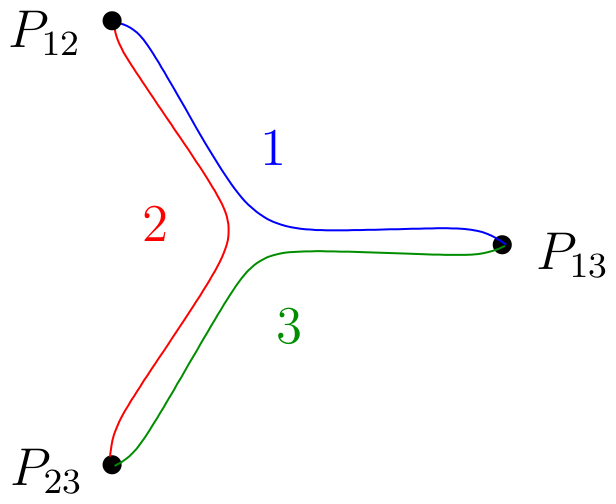
\includegraphics[width=0.35\linewidth]{fig01.png}
  \caption{Morse 树（原书 p.5）}
  \label{fig:1}
\end{figure}
\end{thmenv}

% [Tutor Note: 图 1 中边上的数字 1、2、3 是三个对象的标号（对应图 2 的 $L_1,L_2,L_3$ 即圆盘的三段边界弧），不是边的编号。每条边另带双指标 $(a,b)$ 与方向：$P_{12}$、$P_{23}$ 是叶，$P_{13}$ 是根，方向由叶指向根；方向读反，复合的输入与输出就对调。]

下面这张更细致的图解释这棵树的来源。它来自 $T^*X$ 中 Lagrange 子流形（形如 $L_a=\mathrm{graph}(\epsilon\,\mathrm{d}F_a)$）的 Fukaya 范畴，该范畴的复合映射由全纯圆盘的计数给出：

\begin{figure}[htbp]
  \centering
  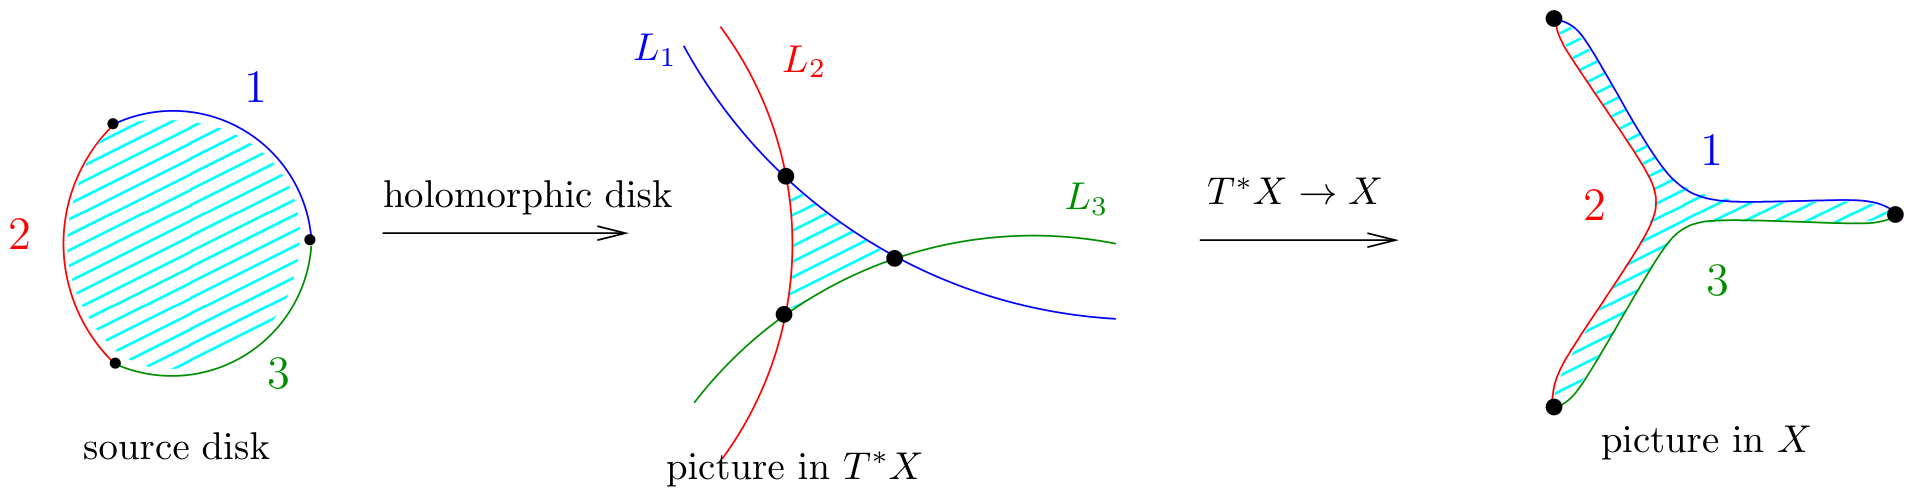
\includegraphics[width=0.76\linewidth]{fig02.png}
  \caption{$X$ 中的 Morse 树：$T^*X$ 中全纯圆盘在 $\epsilon\to0$ 极限下的投影（原书 p.6）}
  \label{fig:2}
\end{figure}

% [Tutor Note: 图 2 中间那幅画在 $T^*X$ 里：$L_a=\mathrm{graph}(\epsilon\,\mathrm{d}F_a)$ 是恰当 Lagrange 子流形，投影 $T^*X\to X$ 把它压到 $X$ 上。$\epsilon\to0$ 时全纯圆盘的面积趋于零，圆盘的极限是梯度流树；这里的“全纯”一律指伪全纯（见第 1 节脚注 1）。紧性论证原文未写，可参看 \cite{fukayaoh}。]

把这张图稍作修改，就得到复合映射
\[
  m\colon\Mor(F_1,F_2)\otimes\Mor(F_2,F_2)\otimes\Mor(F_2,F_3)\to\Mor(F_1,F_3)
\]
的图景；其中用到 $X$ 上（相应地，$T^*X$ 中某个 Lagrange 子流形上）的一条奇异链 $Z\in\Mor(F_2,F_2)$：

\begin{figure}[htbp]
  \centering
  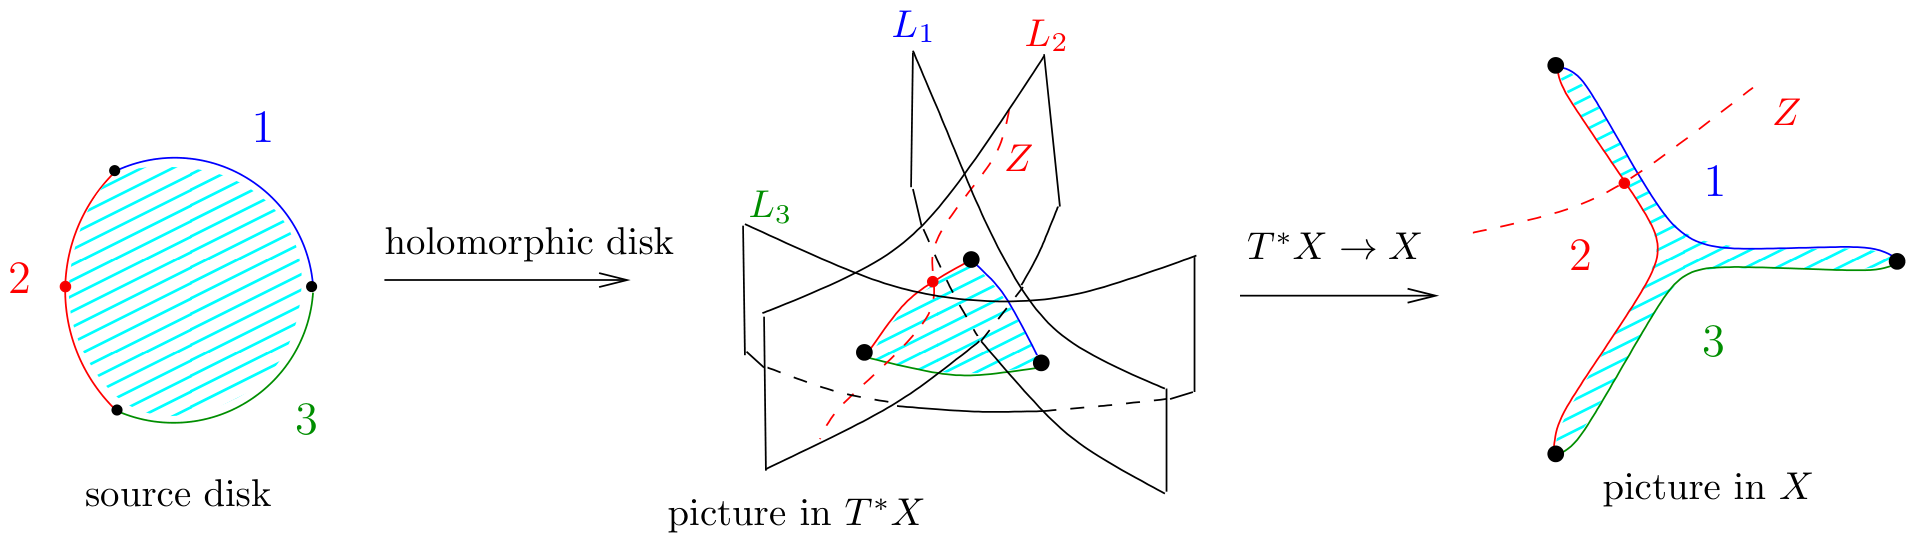
\includegraphics[width=0.76\linewidth]{fig03.png}
  \caption{全纯圆盘与 Morse 树同一条链相交（原书 p.6）}
  \label{fig:3}
\end{figure}

\begin{thmenv}{例}{2}\label{ex:2}
复合映射
\[
  m\colon\Mor(F_1,F_1)^{\otimes k}\otimes\Mor(F_1,F_2)\otimes\Mor(F_2,F_2)^{\otimes l}\to\Mor(F_1,F_2)
\]
由计数 $F_1-F_2$ 的、与给定一族链（图中虚线）相交的梯度轨道给出：
\begin{figure}[htbp]
  \centering
  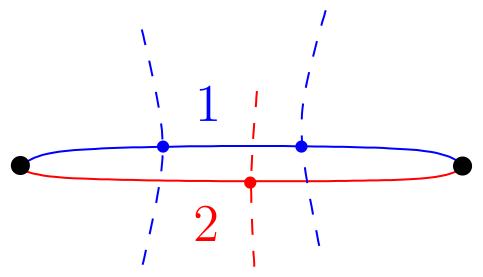
\includegraphics[width=0.20\linewidth]{fig04.png}
  \caption{经过一族链的梯度轨道（原书 p.6）}
  \label{fig:4}
\end{figure}
\end{thmenv}

相应梯度轨道模空间的维数为
\[
  \dim\mathcal M
  =\operatorname{ind}(P)-\operatorname{ind}(P')-1
  -\sum_{\alpha=1}^{k}\bigl(\operatorname{codim}(Z_{\alpha,1})-1\bigr)
  -\sum_{\beta=1}^{l}\bigl(\operatorname{codim}(Z_{\beta,2})-1\bigr).
\]
为使该态射非零，临界点的指标与链的维数须满足平衡条件，即 $\dim\mathcal M=0$。

% [Tutor Note: 维数公式逐项对账：$\operatorname{ind}$ 是 $F_1-F_2$ 的 Morse 指标；$P\to P'$ 的轨道模空间维数为 $\operatorname{ind}(P)-\operatorname{ind}(P')$，再减 1 是去掉梯度流的 $\mathbb R$-平移。每个 2 价顶点是一条边与链 $Z$ 的交点：链的余维数为 $c$ 时只贡献 $c-1$ 个条件，因为交点沿 1 维的边可自动滑动。另注意 (1) 按余指标分次，此处用指标，二者只差常数 $\dim X$，差值不变。]

\begin{thmenv}[$A_\infty$ 关系式的一个例子]{例}{3}\label{ex:3}
取 $X$ 为二维球面，$F_{1,2}$ 为两个函数，使 $F_1-F_2$ 是心形球面的高度函数。设 $P,Q$ 为 $F_1-F_2$ 的两个指标为 2 的临界点，$R$ 为指标为 1 的临界点，$S$ 为指标为 0 的临界点，$Z$ 为一条嵌入区间，如下图。

\begin{figure}[htbp]
  \centering
  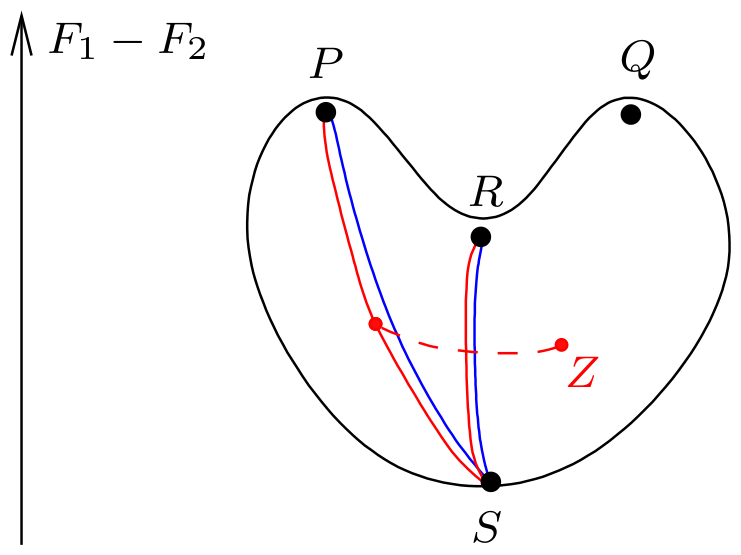
\includegraphics[width=0.30\linewidth]{fig05.png}
  \caption{式~\eqref{eq:8} 的前两项：经过一条链及其边界的梯度轨道（原书 p.7）}
  \label{fig:5}
\end{figure}

有关系式
\begin{equation}\tag{8}\label{eq:8}
  m\bigl(\underbrace{\mathrm{d}_{\mathrm{Morse}}[P]}_{[R]},Z\bigr)
  +m([P],\partial Z)
  +\mathrm{d}_{\mathrm{Morse}}m([P],Z)=0.
\end{equation}
前两项各给出 $S$，且符号相反；第三项为零（因为当 $\widetilde P=S$ 时，模空间 $\mathcal M(P,Z,\widetilde P)$ 是一维的；当 $\widetilde P$ 为其它临界点时，该模空间为空）。这正是 $\Ainf$ 关系式 \eqref{eq:7} 在输入态射 $x_1=[P]$、$x_2=Z$ 下的形式。
\end{thmenv}

% [Tutor Note: 把 (7) 按 $n=2$ 展开：$r=0,s=1$ 给出 $m(\mathrm{d}x_1,x_2)$，$r=1,s=1$ 给出 $m(x_1,\mathrm{d}x_2)$，$r=0,s=2$ 给出 $\mathrm{d}m(x_1,x_2)$，正是 (8) 的三项。注意 $x_2=Z$ 是链，其微分是边界算子，故第二项写作 $m([P],\partial Z)$ 而非 $m([P],\mathrm{d}Z)$；$x_1=[P]$ 是 Morse 链，$\mathrm{d}_{\mathrm{Morse}}[P]=[R]$ 即式 (8) 中的下花括号。]

\subsection{Morse 收缩}\label{sec:2.3}

\begin{takeaway}
\begin{itemize}
  \item \textbf{物理图像}：Morse 收缩把 de Rham 复形压到 Morse 链复形上。$i$ 把临界点打成不稳定流形上的 delta 形式，$p$ 沿稳定流形积分、读回系数，$K$ 沿梯度流积分，给出连接二者的链同伦。
  \item \textbf{数学工具}：$X\times X$ 上的积分核与分布核、奇异支集、正规化数据、光滑化算子 $R_\epsilon$、形变收缩。
  \item \textbf{主要结论}：$(i,p,K)$ 满足 $\mathrm{d}K+K\mathrm{d}=ip-\mathrm{id}$；$K$ 的核是 $\widetilde Y=\cup_{t>0}Y_t$，其边界给出 $Y_{+\infty}-\mathrm{Diag}$；把 $i$、$K$ 光滑化后得到形变收缩 $(i^\epsilon,p,K^\epsilon)$，它是后文证明的关键构件。
\end{itemize}
\end{takeaway}

下一个例子要先回忆 \cite[第 6.5 节]{kontsevichsoibelman} 中的 Morse 收缩构造：它把 de Rham 复形收缩到 Morse 复形。这一构造也是后文几节的关键构件。

设 $F$ 是 $X$ 上的 Morse--Smale 函数，$v$ 是相应的梯度向量场。考虑表达式
\begin{equation}\tag{9}\label{eq:9}
  U(t,\mathrm{d}t)=e^{-t\mathcal L_v}\bigl(1-\mathrm{d}t\,\iota_v\bigr).
\end{equation}
这是 $(0,+\infty)$ 上的非齐次微分形式，取值是作用在 $X$ 的微分形式上的线性算子。\footnote{算子 (9) 是 Morse 拓扑量子力学的演化算子，可理解为度量区间模空间上的一个微分形式，见 \cite{witten,frenkel} 与下文第~\ref{sec:4.1} 节。}下文 $e^{-t\mathcal L_v}$ 一律指沿 $v$ 的流按时间 $-t$ 作拉回。

% [Tutor Note: (9) 中 $\mathcal L_v$ 是李导数，$\iota_v$ 是内乘（interior product）。$U$ 的 0 次部分是拉回 $e^{-t\mathcal L_v}$，1 次部分是 $-\mathrm{d}t\,e^{-t\mathcal L_v}\iota_v$，故 (12) 的负号来自这里；$\int_0^\infty U(t,\mathrm{d}t)$ 只取 $\mathrm{d}t$ 分量，即在 $(0,+\infty)$ 上积一个 1 次形式。把 $\iota_v$ 从 $e^{-t\mathcal L_v}$ 右边挪到左边不变号，因为 $v$ 在自身的流下不变：$e^{-t\mathcal L_v}\iota_v=\iota_v e^{-t\mathcal L_v}$。]

\textbf{未正规化的 Morse 收缩。}\quad 考虑如下三个映射。

\begin{itemize}
  \item 嵌入映射 $i\colon \mathrm{MC}^j(F,\mathbb R)\to\Omega^j_{\mathrm{distr}}(X)$，即把实系数 Morse 复形映入分布形式。它把 $F$ 的余指标为 $j$ 的临界点 $P$ 映为 $P$ 的不稳定流形上的 delta 形式（又称 Lefschetz thimble，莱夫希茨顶针）：
  \begin{equation}\tag{10}\label{eq:10}
    i\colon[P]\mapsto\delta_{\mathrm{Unstab}P}.
  \end{equation}
  \item 投影 $p\colon\Omega^j_{\mathrm{distr}}(X)\to \mathrm{MC}^j(F,\mathbb R)$ 由下式定义：
  \begin{equation}\tag{11}\label{eq:11}
    p\colon\omega\mapsto\sum_{P\in\mathrm{Crit}(F)}
    \Bigl(\int_{\mathrm{Stab}_P}\omega\Bigr)\cdot[P],
  \end{equation}
  其中 $\mathrm{Stab}_P\subset X$ 是 $P$ 的稳定流形。线性算子 $p$ 稠密定义，并满足 $p\circ i=\mathrm{id}_{MC(F)}$。
  \item 链同伦 $K\colon\Omega^j_{\mathrm{distr}}(X)\to\Omega^{j-1}_{\mathrm{distr}}(X)$ 定义为
  \begin{equation}\tag{12}\label{eq:12}
    K=\int_0^\infty U(t,\mathrm{d}t)
    =-\int_0^\infty \mathrm{d}t\,\iota_v e^{-t\mathcal L_v}
    \colon\ \Omega^j_{\mathrm{distr}}(X)\to\Omega^{j-1}_{\mathrm{distr}}(X).
  \end{equation}
  它同样是稠密定义的算子，并满足链同伦性质
  \begin{equation}\tag{13}\label{eq:13}
    \mathrm{d}K+K\mathrm{d}=ip-\mathrm{id}.
  \end{equation}
\end{itemize}

% [Tutor Note: $i$ 用不稳定流形、$p$ 用稳定流形，二者不可互换。$p\circ i=\mathrm{id}$ 的道理是：$\delta_{\mathrm{Unstab}_Q}$ 的余维数为 $\operatorname{ind}Q$，沿维数为 $\operatorname{ind}P$ 的 $\mathrm{Stab}_P$ 积分，只有 $\operatorname{ind}P=\operatorname{ind}Q$ 时可能非零；此时 $P\to Q$ 的梯度轨道必为常值，故只有 $P=Q$ 贡献 1。]

下面给出 (13) 的证明梗概：把 $U$ 写成 $U=e^{-(\mathrm{d}_t+[\mathrm{d}_X,-])(t\iota_v)}$，即可看出 $U$ 满足
\begin{equation}\tag{14}\label{eq:14}
  \bigl(\mathrm{d}_t+[\mathrm{d}_X,-]\bigr)U=0.
\end{equation}
于是
\[
  [\mathrm{d}_X,K]=-\int_0^\infty[\mathrm{d}_X,U]
  =\int_0^\infty \mathrm{d}_t U
  =U(+\infty)-U(0)=U(+\infty)-\mathrm{id}.
\]
我们还需说明
\begin{equation}\tag{15}\label{eq:15}
  U(+\infty)=i\circ p.
\end{equation}

% [Tutor Note: $U=e^{-(\mathrm{d}_t+[\mathrm{d}_X,-])(t\iota_v)}$ 是简写，不是通常的算子指数：指数里的因子并不交换。用 $[\mathrm{d},\iota_v]=\mathcal L_v$ 可算出 $(\mathrm{d}_t+[\mathrm{d}_X,-])(t\iota_v)=t\mathcal L_v+\mathrm{d}t\,\iota_v$；作者实际取的定义是 (9)，两种写法给出同一个满足 (14) 的形式。]

为此注意，算子 $U(t,\mathrm{d}t)$ 在 $(0,+\infty)$ 方向上的 0 次形式分量是积分算子，其分布核为 $\delta_{Y_t}$，其中
\begin{equation}\tag{16}\label{eq:16}
  Y_t=\{(x,y)\in X\times X\mid x=\mathrm{Flow}_t(v)(y)\}\subset X\times X
\end{equation}
是由点对 $(x,y)$ 构成的子流形：从 $y$ 出发的梯度轨道经过时间 $t$ 后到达 $x$。当 $t\to+\infty$ 时，我们考察的是由一条耗时极长的梯度轨道相连的点对；这样的轨道就是一条“断裂轨道”（broken trajectory），它贴近某个临界点，$t=+\infty$ 时则恰好穿过该点。因此 $Y_{+\infty}=\cup_P\,\mathrm{Unstab}_P\times\mathrm{Stab}_P$。于是 $U(+\infty)$ 是以 $\sum_P\delta_{\mathrm{Unstab}P}(x)\delta_{\mathrm{Stab}P}(y)$ 为分布核的积分算子。逐个核对即知，它与 $i\circ p$ 一致。

% [Tutor Note: 原文 p.8 此处作 the gradient trajectory of starting at y，多一个 of，疑为笔误；译文按 the gradient trajectory starting at y 理解，其余照录。另注意 $\widetilde Y$ 不是子流形：它是映照 $(t,y)\mapsto(\mathrm{Flow}_t(v)(y),y)$ 在 $(0,+\infty)\times X$ 上的像，边界由 $t=0$ 处的 $\mathrm{Diag}$ 与 $t=+\infty$ 处的 $Y_{+\infty}$ 拼成，这里的 $\partial$ 是链（current）意义下的边界。]

我们指出，链同伦算子 $K$ 也可看作积分算子，其分布核是 $\delta_{\widetilde Y}$，其中
\begin{equation}\tag{17}\label{eq:17}
  \widetilde Y=\bigcup_{t>0}Y_t\subset X\times X.
\end{equation}
从这个角度看，(13) 由积分核奇异支集层面上的关系 $\partial\widetilde Y=Y_{+\infty}-\mathrm{Diag}$ 直接推出，其中 $\mathrm{Diag}=\{(x,x)\}\subset X\times X$ 是对角线。

\textbf{正规化的 Morse 收缩。}\quad 下面需要引入正规化数据。取一族闭形式 $\rho_\epsilon\in\Omega^{\dim X}(X\times X)$，以 $\epsilon>0$ 为参数，支在 $X\times X$ 中对角线 $\mathrm{Diag}$ 的 $\epsilon$-邻域 $N_\epsilon$ 内，其上同调类是 $[\mathrm{Diag}]$ 这一同调类的 Poincaré 对偶。记 $R_\epsilon\colon\Omega^\bullet_{\mathrm{distr}}(X)\to\Omega^\bullet(X)$ 为“光滑化（smearing）算子”，即由积分核 $\rho_\epsilon$ 定义的线性算子，它把分布形式送到光滑形式。于是对一条链 $Z$，有正规化的（光滑化）delta 形式
\[
  \delta^\epsilon_Z:=R_\epsilon(\delta_Z),
\]
它支在 $Z$ 的 $\epsilon$-邻域内。若链 $Z_1$、$Z_2$ 横截相交，且交为 0-链，则 $\epsilon$ 充分小时有
\begin{equation}\tag{18}\label{eq:18}
  \int_X\delta^\epsilon_{Z_1}\wedge\delta^\epsilon_{Z_2}
  =\int_X\delta^\epsilon_{Z_1}\wedge\delta_{Z_2}
  =\#(Z_1\cap Z_2),
\end{equation}
即交点的带符号计数。

% [Tutor Note: (18) 中间的等号关键是 $R_\epsilon$ 与恒等映射链同伦：$R_\epsilon-\mathrm{id}=\mathrm{d}h_\epsilon+h_\epsilon\mathrm{d}$，而 $\delta^\epsilon_{Z_1}$ 闭，被积式又是顶次形式。于是把 $\delta^\epsilon_{Z_2}$ 换回 $\delta_{Z_2}$ 只差一个恰当形式的积分，在闭流形 $X$ 上为零。原文只写“$\epsilon$ 充分小”，这一步省略了。]

还可构造（见 \cite[第 6.5 节]{kontsevichsoibelman} 的引理 2）一族算子 $h_\epsilon\colon\Omega^\bullet(X)\to\Omega^{\bullet-1}(X)$，其积分核支在 $N_\epsilon$ 内，且满足
\[
  \mathrm{d}h_\epsilon+h_\epsilon\mathrm{d}=R_\epsilon|_{\Omega(X)}-\mathrm{id}.
\]
de Rham 复形 $(\Omega(X),\mathrm{d})$ 到实系数 Morse 链复形 $(\mathrm{MC}(F,\mathbb R),\mathrm{d}_{\mathrm{Morse}})$ 有一个形变收缩，由下面三个映射给出。

\begin{itemize}
  \item 正规化的嵌入映射 $i^\epsilon\colon \mathrm{MC}^j(F,\mathbb R)\to\Omega^j(X)$ 把 $F$ 的余指标为 $j$ 的临界点 $P$ 映为 $P$ 的不稳定流形上的 $\epsilon$-光滑化 delta 形式：
  \begin{equation}\tag{19}\label{eq:19}
    i^\epsilon\colon[P]\mapsto\delta^\epsilon_{\mathrm{Unstab}P}.
  \end{equation}
  \item 投影 $p\colon\Omega^j(X)\to \mathrm{MC}^j(F,\mathbb R)$ 仍由式~\eqref{eq:11} 定义，只是限制在光滑形式上。此时 $\epsilon$ 充分小就有 $p\circ i^\epsilon=\mathrm{id}_{MC(F)}$。
  \item 正规化的链同伦 $K^\epsilon\colon\Omega^j(X)\to\Omega^{j-1}(X)$ 定义为
  \begin{equation}\tag{20}\label{eq:20}
    K^\epsilon=R_\epsilon\circ K+h_\epsilon,
  \end{equation}
  其中 $K$ 由式~\eqref{eq:12} 给出并限制在光滑形式上。它满足性质
  \begin{equation}\tag{21}\label{eq:21}
    \mathrm{d}K^\epsilon+K^\epsilon\mathrm{d}=i^\epsilon p-\mathrm{id}.
  \end{equation}
\end{itemize}

我们把上面定义的三个映射
\begin{equation}\tag{22}\label{eq:22}
  K^\epsilon\ \curvearrowright\ (\Omega(X),\mathrm{d})
  \ \underset{p}{\overset{i^\epsilon}{\rightleftharpoons}}\
  (\mathrm{MC}(F),\mathrm{d}_{\mathrm{Morse}})
\end{equation}
称为与 Morse 函数 $F$ 相伴的（正规化的）Morse 收缩。

% [Tutor Note: 正规化的动机：未正规化的 $i$ 取值在分布形式中（含 delta），而 $p$ 只定义在光滑形式上；后文的树形求和要反复做形式乘法，故必须先把对象换成光滑的。$K^\epsilon=R_\epsilon K+h_\epsilon$ 中的 $h_\epsilon$ 不是可选项：它恰好补上 $R_\epsilon$ 与 $\mathrm{id}$ 之间的链同伦缺口，缺了它 (21) 不成立。]

\endinput

% =====================================================================
%  第 2.4–2.6 节（原书 p.10–14）
% =====================================================================

% ===== 第 2.4 节（原书 p.10–12） =====
\subsection{例：用闭链形变 Morse 微分}\label{sec:2.4}

\begin{takeaway}
\begin{itemize}
  \item \textbf{物理图像}：允许复合映射的输入中含闭链，相当于让梯度轨道在途中穿过给定的子流形；生成参数 $T_\alpha$ 记录轨道穿过了哪些闭链。
  \item \textbf{数学工具}：高阶复合的生成函数 $m(T)$、Maurer--Cartan 方程、同调扰动引理（经 Morse 收缩把 de Rham 复形上的扰动 $\mathrm{d}_2$ 转移到 Morse 复形上）。
  \item \textbf{主要结论}：$\mathrm{d}_{\mathrm{Morse}}+m(T)$ 仍是微分，即式~\eqref{eq:25}；在 $X=S^1$ 的玩具例子中形变给出 $e^T-1$；重复闭链的位移正规化会带来有理系数。
\end{itemize}
\end{takeaway}

考虑只有两个对象 $F_1$、$F_2$ 的范畴 $\mathbb{F}$。设 $\{P_i\}$ 是 $F=F_1-F_2$ 的临界点。固定 $X$ 上的一族闭链 $\{C_\alpha\}$，把它们看作 $\Mor(F_2,F_2)$ 中的元素。考虑高阶复合的生成函数
\begin{equation}\tag{23}\label{eq:23}
  m\colon\ \Mor(F_1,F_2)\otimes\Mor(F_2,F_2)^{\otimes k}\ \to\ \Mor(F_1,F_2),
\end{equation}
它由下式给出
\begin{equation}\tag{24}\label{eq:24}
  m_i^j(T)=\sum_{k\ge 1}\ \sum_{\alpha_1,\dots,\alpha_k}
  \#\mathcal M(P_i,C_{\alpha_1},\dots,C_{\alpha_k},P_j)\,T_{\alpha_1}\cdots T_{\alpha_k},
\end{equation}
其中 $T_\alpha$ 是生成参数，其奇偶性与 $C_\alpha$ 的余维数的奇偶性相反（也可以按 $|T_\alpha|=1-\operatorname{codim}C_\alpha$ 赋予 $\mathbb Z$-次数）。因此，式 (24) 中 $T$ 的各单项式的系数，就是 $F$ 从 $P_i$ 到 $P_j$、且经过给定闭链的梯度轨道的计数。

% [Tutor Note: 此处极易把符号搞反：正确的约定是 $|T_\alpha|=1-\operatorname{codim}C_\alpha$，而不是 $\operatorname{codim}C_\alpha-1$。按前者，例 4 中 $\operatorname{codim}C=1$ 给出 $|T|=0$，故 $e^T$ 的展开不带附加符号；若按后者则 $|T|=-2$，$m(T)$ 的奇偶性与 $e^T-1$ 的符号会整体改变，式 (25) 的符号也随之失配。]

生成函数 (24) 是 $\mathbb Q\otimes\Mor(F_1,F_2)[[T_\alpha]]$ 上某个自同态 $m(T)$ 的矩阵元（式中的 $\mathbb Q$ 因子的来由见注~\ref{rem:2.1}）。$\Ainf$ 关系式 (7) 推出 Maurer--Cartan 方程
\begin{equation}\tag{25}\label{eq:25}
  [\mathrm{d}_{\mathrm{Morse}},m(T)]+m(T)^2=0,
\end{equation}
参看 \cite{lysov}。等价地说，$\mathrm{d}_{\mathrm{Morse}}+m(T)$ 是一个微分。

% [Tutor Note: 为什么模型中要张量 $\mathbb Q$：Morse 链复形本来定义在 $\mathbb Z$ 上，但重复闭链的位移正规化（注~\ref{rem:2.1}）会产生 $1/k!$ 型的有理系数，$m(T)$ 因而只在张量 $\mathbb Q$ 之后才成为良定义的自同态。若忽略这一点，会误以为 $m(T)$ 保持整系数，进而误判整系数版本是否存在。]

我们指出，“生成函数” $m(T)$ 遗漏了复合映射 (23) 的一部分数据：它隐含了对闭链的对称化，即忘掉了梯度轨道与这些闭链相交的先后次序，因为生成参数 $T_\alpha$ 被当作超交换的。

\begin{thmenv}{注}{2.1}\label{rem:2.1}
当同一个闭链在式 (24) 中作为参数重复出现若干次时，横截性假设（假设~\ref{ass:2.2}）失效。为排除这一失效，我们把该闭链的若干份副本作轻微位移，并对“哪一份副本得到哪个位移”作对称化。例如：只考虑一条余维数为 1 的闭链 $C$，并考虑式 (24) 中的项 $\#\mathcal M(P_i,C,C,P_j)\,T^2$。把 $C$ 的两份副本分别位移为 $C'$ 与 $C''$ 再作对称化，得到 $\tfrac12\bigl(\#\mathcal M(P_i,C',C'',P_j)+\#\mathcal M(P_i,C'',C',P_j)\bigr)T^2$。也就是说，我们计数从 $P_i$ 到 $P_j$ 的梯度轨道：其中先经过 $C'$、再经过 $C''$ 的轨道带权重 $T^2/2$，先经过 $C''$、再经过 $C'$ 的轨道也带权重 $T^2/2$。位移很小时，这等于 $\tfrac12\sum_\gamma(\#(\gamma\cap C))^2$，其中求和遍历从 $P_i$ 到 $P_j$ 的梯度轨道 $\gamma$。我们注意到，这种对重复闭链的正规化，使 $m(T)$ 中出现有理（而非整数）系数。
\end{thmenv}

% [Tutor Note: 对称化给出的权重是 $T^2/2$，不是笔误：$C$ 的两份副本各得 $1/2$ 的权重，分母上的 $2=2!$；推广到 $k$ 份相互重复的副本时权重为 $1/k!$，这正是例 4 与本节第二个脚注（原书脚注 8）中系数 $1/k!$ 的来源。只有当位移足够小时，对称化的结果才等于 $\tfrac12\sum_\gamma(\#(\gamma\cap C))^2$。]

\begin{thmenv}{例}{4}\label{ex:4}
一个玩具例子如下：取 $X=S^1$，把 $X$ 作为单位圆嵌入 $\mathbb R^2$，$F$ 取相应的高度函数；它有指标 1 的临界点 $P$ 与指标 0 的临界点 $Q$。设 $C$ 为一个 0-闭链，即 $S^1\setminus\{P,Q\}$ 上的某个点；设 $T$ 是相应的生成参数（交换，次数为 $|T|=0$）。
\end{thmenv}

\begin{figure}[htbp]
  \centering
  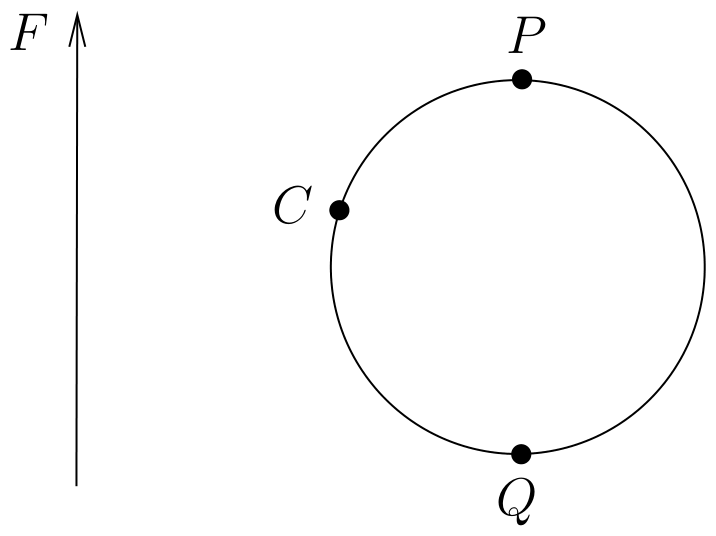
\includegraphics[width=0.42\linewidth]{fig06.png}
  \caption{带闭链 $C$ 的圆（原书 p.11）}
  \label{fig:6}
\end{figure}

此时 Morse 微分 $\mathrm{d}_{\mathrm{Morse}}=0$，但形变后的 Morse 微分 $\mathrm{d}_{\mathrm{Morse}}+m(T)$ 为
\[
  \mathrm{d}_{\mathrm{Morse}}+m(T)\colon\quad
  \begin{cases}
    [P]\mapsto (e^{T}-1)[Q],\\
    [Q]\mapsto 0.
  \end{cases}
\]
这里的形变来自
\[
  m_P^Q(T)=\#\mathcal M(P,C,Q)\,T+\#\mathcal M(P,C,C,Q)\,T^2+\cdots
  =T+\tfrac12T^2+\cdots=e^T-1.
\]
对闭链 $C$ 的每一组副本位移，从 $P$ 到 $Q$ 且按正确次序经过这些副本的梯度轨道要么恰有一条，要么一条也没有。对位移作对称化之后，就得到系数 $1/k!$。

% [Tutor Note: 为什么 $\mathrm{d}_{\mathrm{Morse}}=0$：在圆上，从极大点 $P$ 到极小点 $Q$ 恰有两条梯度轨道（沿两侧各一段半圆），二者定向相反，带符号计数相互抵消。而 $m_P^Q(T)$ 数的是经过闭链副本的轨道：对每组位移，按正确次序经过副本的轨道恰有一条，对称化后得 $1/k!$，累加即 $e^T-1=\sum_{k\ge 1}T^k/k!$。]

\textbf{通过同调扰动引理的进路。}\quad 式 (25) 可以这样证明：把 $X$ 上的微分形式复形看作双复形，第一个微分是 de Rham 微分 $\mathrm{d}_1=\mathrm{d}$，第二个微分是乘以微分形式
\[
  \mathrm{d}_2=\sum T_\alpha\,\delta^\epsilon_{C_\alpha},
\]
其中 $\delta^\epsilon_{C_\alpha}$ 是闭链的光滑化 delta 形式，见第~\ref{sec:2.3} 节。当各 $C_\alpha$ 的余维数为 1 时，这样的微分叫作 Novikov 微分 $\mathrm{d}_{\mathrm{Novikov}}=\mathrm{d}+\omega$；我们这里用的是它的显然推广。

算子 $m(T)$ 只是把第二个微分诱导到子复形（相对于 $\mathrm{d}_1$）上的结果，所用的是同调扰动引理\footnote{参看 \cite{gugenheim,lambe}。综述可参看 \cite{crainic}。拓扑量子力学的视角另见 \cite{losev}。}与 Morse 收缩。形变后的 de Rham 复形 $(\Omega^\bullet(X)[[T_\alpha]],\mathrm{d}_1+\mathrm{d}_2)$ 与形变后的 Morse 复形 $(\mathrm{MC}^\bullet(F,\mathbb R)[[T_\alpha]],\mathrm{d}_{\mathrm{Morse}}+m(T))$ 拟同构，其中 $m(T)$ 由下式给出：
\begin{equation}\tag{26}\label{eq:26}
  m(T)=p\,\mathrm{d}_2\,i^\epsilon+p\,\mathrm{d}_2K^\epsilon \mathrm{d}_2\,i^\epsilon
  +p\,\mathrm{d}_2K^\epsilon \mathrm{d}_2K^\epsilon \mathrm{d}_2\,i^\epsilon+\cdots
\end{equation}

这里 $(i^\epsilon,p,K^\epsilon)$ 是上面式 (10)、(11)、(12) 中的映射。我们假定 $\epsilon$ 足够小。事实上，把式 (26) 展开，得到
\begin{equation}\tag{27}\label{eq:27}
\begin{aligned}
  m(T)[P_i]={}&
  \lim_{\epsilon\to0}\sum_{j}\sum_{k\ge1}\sum_{\alpha_1,\dots,\alpha_k}
  \left(\int_{\mathrm{Stab}_{P_j}}\delta^\epsilon_{C_{\alpha_k}}
  K^\epsilon\bigl(\delta^\epsilon_{C_{\alpha_{k-1}}}\cdots
  \delta^\epsilon_{C_{\alpha_2}}K^\epsilon
  (\delta^\epsilon_{C_{\alpha_1}}\delta^\epsilon_{\mathrm{Unstab}_{P_i}})\cdots\bigr)
  \right)\\
  &\quad\cdot T_{\alpha_1}\cdots T_{\alpha_k}\cdot[P_j]\\
  ={}&\sum_{j}\sum_{k\ge1}\sum_{\alpha_1,\dots,\alpha_k}
  \#\mathcal M(P_i,C_{\alpha_1},\dots,C_{\alpha_k},P_j)\,
  T_{\alpha_1}\cdots T_{\alpha_k}\cdot[P_j].
\end{aligned}
\end{equation}

最后一个等号是显然的，只有序列 $C_{\alpha_1},\dots,C_{\alpha_k}$ 含重复闭链这一更微妙的情形除外。我们预期，在这种情形下，$\epsilon$-正规化给出的贡献也与注~\ref{rem:2.1} 的计数式规定一致。\footnote{例如在例~\ref{ex:4} 中，这就是一个直接的验证：取第~\ref{sec:2.3} 节意义下的正规化数据，即 $S^1\times S^1$ 上一个支撑在对角线的 $\epsilon$-邻域内的闭 1-形式 $\rho_\epsilon=f_\epsilon(\theta,\theta')\,\mathrm{d}\theta+g_\epsilon(\theta,\theta')\,\mathrm{d}\theta'$，并满足 $\int f_\epsilon\,\mathrm{d}\theta=1$、$\int g_\epsilon\,\mathrm{d}\theta'=-1$（$\theta$ 是 $S^1$ 上的角坐标）。对 $k=1,2,\dots$ 作归纳可证 $(\delta^\epsilon_C K^\epsilon)^{k-1}(\delta^\epsilon_C\delta^\epsilon_{\mathrm{Unstab}P})=\frac{1}{k!}\,\mathrm{d}\theta\,\frac{\mathrm{d}}{\mathrm{d}\theta}\bigl(\int^\theta \mathrm{d}\theta'\,f_\epsilon(\theta',\theta_0)\bigr)^k$，其中 $\theta_0$ 是 0-闭链 $C$ 的位置。由此可得 $\int_{\mathrm{Stab}Q}(\delta^\epsilon_C K^\epsilon)^{k-1}(\delta^\epsilon_C\delta^\epsilon_{\mathrm{Unstab}P})=1/k!$。}因此，带上这一保留条件，式 (26) 与计数式定义 (24) 一致。$\mathrm{d}_{\mathrm{Morse}}+m(T)$ 的平方为零这一事实，于是就是同调扰动引理的直接推论。

% [Tutor Note: 作者说“显然”，实际用到两步：其一，$\epsilon\to0$ 时 $\delta^\epsilon_C$ 弱收敛到 $\delta_C$，$K^\epsilon$ 的积分核收敛到 $\delta_{\widetilde Y}$（式 (17) 与第 2.3 节的正则化构造）；其二，沿 $X^V$ 的积分在横截性下化为交点计数。标准出处是 Gugenheim \cite{gugenheim} 与 Lambe--Stasheff \cite{lambe} 的扰动引理，综述见 Crainic \cite{crainic}。]

% ===== 第 2.5 节（原书 p.12–14） =====
\subsection{Morse 树模空间的相交公式与横截性假设}\label{sec:2.5}

\begin{takeaway}
\begin{itemize}
  \item \textbf{物理图像}：复合映射的模空间可以写成 $X^m$ 中若干拉回链的相交——每条内部边对应 $\widetilde Y_e$，每个 2 价顶点对应一条链 $Z_q$，叶子与根分别对应不稳定流形与稳定流形。
  \item \textbf{数学工具}：投影 $\pi_q,\pi_e,\pi_{\text{leaf}\,i},\pi_{\text{root}}$、链的横截相交、维数公式。
  \item \textbf{主要结论}：相交公式 (28)；横截性假设~\ref{ass:2.2} 成立时 $\mathcal M$ 是光滑整链，维数由式 (28) 后的公式给出；假设失效时模空间维数跳变（例~\ref{ex:5}）。
\end{itemize}
\end{takeaway}

考虑复合映射 (4) 的定义中出现的 Morse 树的模空间 $\mathcal M$。存在一个自然的单射，把该模空间映入 $X^m$：记录 Morse 树的三价顶点在 $X$ 中的位置，以及梯度轨道与链 $Z_{\alpha,a}$ 的交点在 $X$ 中的位置。这里 $m=r-2+\sum_i k_i$ 是相应树中内部顶点（2 价与 3 价）的总数。这一单射的像——因而 $\mathcal M$ 的一个模型——可以用 $X^m$ 中链的相交来描述：
\begin{equation}\tag{28}\label{eq:28}
\begin{aligned}
  &\mathcal M\bigl(\{Z_{\alpha,a_1}\}_{\alpha=1}^{k_1};P_{a_1a_2};
  \{Z_{\alpha,a_2}\}_{\alpha=1}^{k_2};P_{a_2a_3};\cdots;
  P_{a_{r-1}a_r};\{Z_{\alpha,a_r}\}_{\alpha=1}^{k_r};P_{a_1a_r}\bigr)\simeq{}\\
  &\qquad\sum_{\text{trees }T}
  \Biggl(\biggl(\bigcap_{e\in E}\pi_e^{-1}\widetilde Y_e\biggr)
  \cap\biggl(\bigcap_{q\in V_2}\pi_q^{-1}(Z_q)\biggr)
  \cap\biggl(\bigcap_{i=1}^{r-1}\pi_{\mathrm{leaf}\,i}^{-1}
  \bigl(\mathrm{Unstab}_{P_{a_ia_{i+1}}}\bigr)\biggr)
  \cap\pi_{\mathrm{root}}^{-1}\bigl(\mathrm{Stab}_{P_{a_1a_r}}\bigr)\Biggr).
\end{aligned}
\end{equation}

% [Tutor Note: 本段 $m=r-2+\sum_i k_i$ 中的 $m$ 是空间 $X^m$ 的指数（内部顶点总数），与复合映射 $m$ 无关；同段 $Z_{\alpha,a}$ 的下标 $a$ 与临界点 $P_{ab}$ 的双指标也各有含义，读式 (28) 时先分清这两套指标。]

其中：

\begin{itemize}
  \item 求和遍历有 $r-1$ 片叶子的有根树 $T$ 的组合类型。如上所述，边带双色 $(ab)$；沿从叶子 $(a_{i-1},a_i)$ 到叶子 $(a_i,a_{i+1})$ 的路径，会遇到 $k_i$ 个颜色为 $a_i$ 的 2 价顶点（其中叶子 $(a_r,a_1)$ 是根）。假定 $T$ 中的顶点至多为 3 价。
  \item $E$ 是内部边（不与 1 价顶点相邻的边）的集合。$V=V_2\cup V_3$ 是价不等于 1 的顶点的集合；$V_k$ 是 $k$ 价顶点的集合。
  \item 对双色为 $(a,b)$ 的边 $e$，$\widetilde Y_e$ 是与 Morse 函数 $F_a-F_b$ 相联系的 $X\times X$ 中的链 (17)。
  \item 映射 $\pi_q\colon X^V\to X$ 是到第 $q$ 个分量的投影。若 $e$ 是连接顶点 $q_1$ 与 $q_2$ 的边，则 $\pi_e\colon X^V\to X\times X$ 是选取 $X$ 的第 $q_1$ 份与第 $q_2$ 份副本的投影。$\pi_{\mathrm{leaf}\,i}\colon X^V\to X$ 选取由一条边与 $(a_i,a_{i+1})$-叶相连的顶点所对应的分量。同样，$\pi_{\mathrm{root}}\colon X^V\to X$ 选取由一条边与根相连的顶点所对应的分量。
\end{itemize}

% [Tutor Note: $\pi_e^{-1}\widetilde Y_e$ 里的波浪号不能丢：$\widetilde Y_e=\bigcup_{t>0}Y_t$ 是式 (17) 中 $X\times X$ 内的整条扩展轨道族的链，而 $Y_t$ 只是 $t$ 时刻的流动像。$\pi_e$ 把 $X^V$ 投到第 $q_1,q_2$ 份 $X\times X$，$\pi_q$ 只投到单个 $X$，两者的纤维维数不同，把 $\pi_q^{-1}(\widetilde Y_e)$ 写进公式是错的。]

关于临界点与链的序列，使复合映射 (4) 有良好定义的关键横截性假设如下。

\begin{thmenv}{假设}{2.2}\label{ass:2.2}
我们假定：式 (28) 中的输入临界点 $P_{ab}$ 与链 $Z_{\alpha,a}$ 构成的序列，满足对每棵树 $T$，式 (28) 右端的相交都是横截的。
\end{thmenv}

在此假设下，$\mathcal M$ 是 $X^m$ 中一条光滑的整链，其维数为
\[
\begin{aligned}
  \dim\mathcal M={}&\\
  ={}&(\operatorname{coind}(P_{a_1a_r})-1)
  -\sum_{i=1}^{r-1}\bigl(\operatorname{coind}(P_{a_ia_{i+1}})-1\bigr)
  -\sum_{\alpha,k}\bigl(\operatorname{codim}(Z_{\alpha,k})-1\bigr)-1.
\end{aligned}
\]

% [Tutor Note: 疑似笔误：原书 p.13 把维数公式排成两行，第一行以 $\dim\mathcal M=$ 结尾，第二行又以 $=$ 起头，于是等号出现两次。译文照印，未删去第二个等号；按上下文，第一个等号后应直接接第二行的右端。]

\begin{thmenv}{例}{5}\label{ex:5}
非横截复合的一个例子如下：$N=2$，$X$ 是作为 $\mathbb R^3$ 中单位球面实现的 2-球面，$F_1-F_2$ 取 $z$-坐标。临界点是北极 $\mathbf N$ 与南极 $\mathbf S$。设 1-闭链 $C$ 为赤道 $z=0$，$C'$ 为一个 0-闭链，即 $S^2$ 中某处的点。考虑复合 $m(\mathbf N,C,C')$：
\begin{enumerate}
  \item[(1)] 若点 $C'$ 在下半球（但不在 $\mathbf S$ 处），则存在唯一一条由 $\mathbf N$ 连到 $\mathbf S$ 且经过 $C$ 与 $C'$ 的梯度轨道，故 $m(\mathbf N,C,C')=\mathbf S$。
  \item[(2)] 若点 $C'$ 在上半球（但不在 $\mathbf N$ 处），则梯度轨道经过闭链的次序不对，故 $m(\mathbf N,C,C')=0$。
  \item[(3)] 若 $C'$ 在赤道上，横截性假设失效。
  \item[(4)] 若 $C'$ 与两个临界点 $\mathbf N$、$\mathbf S$ 之一重合，横截性假设也失效。此时从 $\mathbf N$ 到 $\mathbf S$ 且经过 $C$ 与 $C'$ 的 Morse 轨道的模空间是一维的，而预期维数为零。
\end{enumerate}
\end{thmenv}

\begin{figure}[htbp]
  \centering
  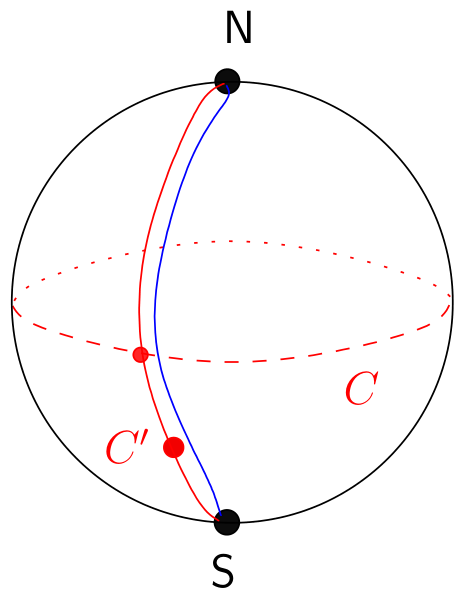
\includegraphics[width=0.30\linewidth]{fig07.png}
  \caption{经过闭链 $C$ 与 $C'$ 的梯度轨道（原书 p.13）}
  \label{fig:7}
\end{figure}

于是，横截性假设在情形 (1)、(2) 中成立，在情形 (3)、(4) 中失效。

% [Tutor Note: “预期维数为零”来自式 (28) 后的维数公式，作者没有写出代入过程：此处 $\operatorname{coind}(\mathbf S)-1=2-1=1$，$-\bigl(\operatorname{coind}(\mathbf N)-1\bigr)=-(0-1)=1$，两条链贡献 $-\bigl((1-1)+(2-1)\bigr)=-1$，最后再减 1，合计 $1+1-1-1=0$。实际模空间是一维的，故横截性必然失效。]

% ===== 第 2.6 节（原书 p.14） =====
\subsection{复合映射系数的积分公式}\label{sec:2.6}

\begin{takeaway}
\begin{itemize}
  \item \textbf{物理图像}：把相交公式里的每条链换成它的 delta 分布形式，相交数就变成 $X^V$ 上的积分；对 $\mathbb R_+^E$ 积分后，每条内部边只剩其扩展轨道族的积分核 $\delta_{\widetilde Y_e}$。
  \item \textbf{数学工具}：分布形式、积分核、波前集、横截性。
  \item \textbf{主要结论}：积分公式 (29) 与 (31)；积分号下分布形式之积有定义，由假设~\ref{ass:2.2} 保证的波前集横截性给出。
\end{itemize}
\end{takeaway}

作为式 (28) 的推论，在横截性假设下，式 (4) 中作为系数出现的 Morse 树的数目满足如下积分公式：
\begin{equation}\tag{29}\label{eq:29}
\begin{aligned}
  &\#\mathcal M\bigl(\{Z_{\alpha,a_1}\}_{\alpha=1}^{k_1};P_{a_1a_2};
  \{Z_{\alpha,a_2}\}_{\alpha=1}^{k_2};P_{a_2a_3};\cdots;
  P_{a_{r-1}a_r};\{Z_{\alpha,a_r}\}_{\alpha=1}^{k_r};P_{a_1a_r}\bigr)\\
  &\quad=\sum_{\text{trees }T}\int_{\mathbb R_+^E}\int_{X^V}
  \prod_{e\in E}\widetilde\pi_e^*\eta_e
  \prod_{q\in V_2}\pi_q^*(\delta_{Z_q})
  \prod_{i=1}^{r-1}\pi_{\mathrm{leaf}\,i}^*
  \bigl(\delta_{\mathrm{Unstab}_{P_{a_ia_{i+1}}}}\bigr)
  \cdot\pi_{\mathrm{root}}^*\bigl(\delta_{\mathrm{Stab}_{P_{a_1a_r}}}\bigr).
\end{aligned}
\end{equation}
记号与式 (28) 相同。此外：

\begin{itemize}
  \item 分布形式
  \begin{equation}\tag{30}\label{eq:30}
    \eta_e=(1-\mathrm{d}t\,\iota_v)\delta(Y_t)\in\Omega^{\dim X}(\mathbb R_+\times X\times X)
  \end{equation}
  是式 (9) 中定义的算子值微分形式 $U$ 的积分核；$U$ 与 $F_a-F_b$ 的梯度向量场相联系，其中 $(a,b)$ 是边 $e$ 的双色。
  \item 若 $e$ 是连接顶点 $q_1$ 与 $q_2$ 的边，则映射 $\widetilde\pi_e\colon\mathbb R_+^E\times X^V\to\mathbb R_+\times X\times X$ 是选取 $X$ 的第 $q_1$ 份与第 $q_2$ 份副本、以及 $\mathbb R_+$ 的第 $e$ 份副本的投影。
\end{itemize}

把 $\mathbb R_+^E$ 上的积分算出来，就可以把式 (29) 写成
\begin{equation}\tag{31}\label{eq:31}
\begin{aligned}
  \#\mathcal M={}&\sum_{\text{trees }T}\int_{X^V}
  \prod_{e\in E}\pi_e^*\delta_{\widetilde Y_e}
  \prod_{q\in V_2}\pi_q^*(\delta_{Z_q})
  \prod_{a=1}^{N-1}\pi_{\mathrm{leaf}\,a}^*
  \bigl(\delta_{\mathrm{Unstab}_{P_{a_ia_{i+1}}}}\bigr)\\
  &\quad\cdot\pi_{\mathrm{root}}^*\bigl(\delta_{\mathrm{Stab}_{P_{a_1a_r}}}\bigr).
\end{aligned}
\end{equation}
这里 $\delta_{\widetilde Y_e}$ 是非正规化 Morse 同伦 (12) 的积分核。式 (31) 积分号下各分布形式之积有良好定义，因为由假设~\ref{ass:2.2}，各波前集横截。

% [Tutor Note: 疑似笔误：式 (31) 的乘积写作 $\prod_{a=1}^{N-1}$，但被积函数里是 $\delta_{\mathrm{Unstab}_{P_{a_ia_{i+1}}}}$，下标是 $i$ 而不是 $a$；照式 (29) 应为 $\prod_{i=1}^{r-1}$，或把被积函数的下标改成 $P_{a\,a+1}$。另外这里的 $N-1$ 与式 (29) 的 $r-1$ 也不一致（$N$ 是对象个数，$r$ 是树中叶子个数）。译文照原样排印，未擅改。]

% [Tutor Note: 末句的“波前集横截”是关键：Hörmander 的波前集理论断言，两个分布之积有定义当且仅当二者的波前集沿对角逐点横截。$\delta_Z$ 的波前集是 $Z\subset X$ 的余法丛，故对 $X^V$ 上各拉回形式的乘积而言，横截性条件恰是假设~\ref{ass:2.2} 的相交横截性。可参看 Hörmander《The Analysis of Linear Partial Differential Operators》第 8 章。]

\endinput

% =====================================================================
%  第 2.7 节 与第 3 节  旁注 · 用二次量子化证明 A∞ 关系式（原书 p.14–20）
% =====================================================================
\subsection{旁注：$\Mor(F_a,F_a)$ 的其它可能模型}\label{sec:2.7}

\begin{takeaway}
\begin{itemize}
  \item \textbf{物理图像}：对象到自身的态射空间可以另取模型，或用微分形式，或用奇异上链。前者让复合处处有定义，后者让余边界算子与 cup 积处处有定义。
  \item \textbf{数学工具}：de Rham dg 代数 $\Omega^\bullet(X)$、积分公式~\eqref{eq:29}、奇异上链复形 $C^\bullet_{\mathrm{sing}}(X,\mathbb Z)$、cup 积。
  \item \textbf{主要结论}：两个变体各有代价，前者丢掉整结构与计数味道，后者仍只给出部分定义的复合；只有链模型保留计数几何。
\end{itemize}
\end{takeaway}

(i) 可以考虑 $\Ainf$ 范畴 $\mathbb{F}$ 的一个变体 $\mathbb{F}_\Omega$：其中对象的自同态空间 $\Mor(F_a,F_a)$ 取为 de Rham dg 代数 $\Omega^\bullet(X)$。复合映射按式~\eqref{eq:4} 定义，只把链 $Z_{\alpha,a}$ 换成微分形式 $\omega_{\alpha,a}\in\Omega^\bullet(X)$，把系数 $\#\mathcal M$ 按积分公式~\eqref{eq:29} 定义（代替第~\ref{sec:2.1} 节的计数定义），并把 $\delta_{Z_q}$ 换成光滑形式 $\omega_q$。好处在于：只要函数 $F_a$ 处于一般位置，所得的 $\Ainf$ 范畴 $\mathbb{F}_\Omega$ 中复合就总有定义。代价是整结构丢失：态射空间与复合都是 $\mathbb R$ 上的上链复形，而不是 $\mathbb Z$ 上的。此外，复合的计数味道在这个模型里也丢掉了。我们还要指出：把 $\mathbb{F}_\Omega$ 中的复合限制到链的 $\epsilon$-光滑化 delta 形式上，就得到 $\mathbb{F}$ 中的复合。

% [Tutor Note: 这里三类 $\delta$ 的含义不同：$\delta_{Z_q}$ 是链的 delta 形式（对链积分即数交点），$\delta_{\mathrm{Unstab}_{P_{a_ia_{i+1}}}}$ 与 $\delta_{\mathrm{Stab}_{P_{a_1a_r}}}$ 是稳定、不稳定流形的 delta 形式，而 $\epsilon$-光滑化 delta 形式是链的 delta 形式的正则化。把三类混为一谈，就会误以为链与临界点在这个变体里地位相同。]

(ii) 另一种方案是把对象的自同态空间定义为奇异上链而非链，即 $\Mor(F_a,F_a)=C^\bullet_{\mathrm{sing}}(X,\mathbb Z)$，其 dg 代数结构由余边界算子与 cup 积给出。\footnote{P.~M. 感谢 Stephan Stolz 提出这一点。}这些运算总有定义，不需要额外的横截性要求。然而，要定义更一般的复合映射，仍需加上横截性要求。因此得到的仍是一个复合部分定义的 $\Ainf$ 范畴。

% [Tutor Note: 为什么 cup 积不需要横截性、而链的相交需要？cup 积是上链层面的代数运算，任意两条上链都可以相乘；链的相交则要求子流形横截，否则交点集不是离散的，计数无意义。但高阶复合仍要数 Morse 树与链的交，所以横截性没有消失，只是从基本运算挪到了复合这一步——这正是作者说「仍得到部分定义的范畴」的原因。]

\section{用二次量子化证明 $\Ainf$ 关系式}\label{sec:3}

\begin{takeaway}
\begin{itemize}
  \item \textbf{物理图像}：把范畴 $\mathbb{F}$ 的高阶复合看成某个 dg 代数经同伦转移得到的高阶乘法；在物理上，同一个结构就是 BF 理论的有效作用量，即二次量子化。
  \item \textbf{数学工具}：Morse 收缩与收缩三元组、Kontsevich--Soibelman 树形求和公式、Batalin--Vilkovisky 形式、奇辛纤维化上的纤维 BV 积分、Feynman 图展开。
  \item \textbf{主要结论}：诱导的乘法 $\mu$ 满足 $\Ainf$ 关系式~\eqref{eq:36}，由式~\eqref{eq:35} 即得范畴 $\mathbb{F}$ 的 $\Ainf$ 关系式~\eqref{eq:7}。BF 理论一侧的 $L_\infty$ 括号经式~\eqref{eq:47} 恢复 $\mu_n$，给出同一定理的场论证明。
\end{itemize}
\end{takeaway}

% [Tutor Note: 本节与第 4 节是定理~\ref{thm:1} 的两个独立证明。核心工具是同伦转移的存在性：给定收缩数据 $(i,\mathrm{p},K)$ 后，只要树形求和按次数逐次有限（Morse 收缩经正规化后满足这一条），dg 代数结构就能搬到 $\mathbb{M}$ 上。标准陈述是同调扰动引理，见 \cite{crainic,gugenheim,lambe}；树形求和的具体形状即 Kontsevich--Soibelman 公式 \cite{kontsevichsoibelman}。]

\subsection{同伦转移证明}\label{sec:3.1}

\begin{takeaway}
\begin{itemize}
  \item \textbf{物理图像}：把取值于微分形式的 $N\times N$ 矩阵 dg 代数收缩到 Morse 复形 $\mathbb{M}$，再用树的和定义高阶乘法，这就是同伦转移。
  \item \textbf{数学工具}：Morse 收缩式~\eqref{eq:20}、收缩三元组 $(\mathrm{i},\mathrm{p},K)$、Kontsevich--Soibelman 树形公式~\eqref{eq:33}。
  \item \textbf{主要结论}：诱导的 $\mu$ 与范畴复合 $m$ 逐项相等（式~\eqref{eq:35}，$\epsilon$ 对每个复合分别取充分小），于是 $\Ainf$ 关系式~\eqref{eq:36} 推出范畴关系式~\eqref{eq:7}。
\end{itemize}
\end{takeaway}

考虑如下微分分次（dg）代数：取 $X$ 上微分形式的超交换 de Rham dg 代数与 $N\times N$ 矩阵的结合代数 $M_N$ 的张量积。作为向量空间，它是
\[
V=\bigoplus_{a,b=1}^{N}\Omega_{ab},
\]
其中每个空间 $\Omega_{ab}$ 都同构于 $X$ 上微分形式的空间。现在，对 $a\neq b$，考虑（正规化）Morse 收缩：它把空间 $\Omega_{ab}$ 收缩到函数 $F_a-F_b$ 的 Morse 链上，其同伦取式~\eqref{eq:20}。于是得到 $V$ 到复形
\[
\mathbb{M}=\bigoplus_{a,b}\mathbb{M}_{ab},
\qquad\text{其中}\quad
\mathbb{M}_{ab}=
\begin{cases}
\mathrm{MC}(F_a-F_b,\mathbb{R}), & a\neq b,\\
\Omega_{aa}, & a=b
\end{cases}
\]
的收缩。

我们再次得到一个三元组，即嵌入、投影与链同伦：
\begin{equation}\tag{32}\label{eq:32}
K\;\curvearrowright\;V\ \underset{\mathrm{p}}{\overset{\mathrm{i}}{\rightleftarrows}}\ \mathbb{M},
\end{equation}
它们由 $(a,b)$-分块（$a\neq b$）上的正规化 Morse 收缩映射给出，在 $(a,a)$-分块上取平凡（$\mathrm{i}=\mathrm{p}=\mathrm{id}$，$K=0$）。

% [Tutor Note: 收缩三元组的标准条件是 $\mathrm{p}\,\mathrm{i}=\mathrm{id}_{\mathbb{M}}$ 与 $\mathrm{i}\,\mathrm{p}-\mathrm{id}_V=d_VK+Kd_V$（符号随分级约定略有出入），且 $K$ 的次数为 $-1$。$(a,a)$ 分块取 $\mathrm{i}=\mathrm{p}=\mathrm{id}$、$K=0$，是全篇「增强」的来源：$F_a-F_a\equiv0$ 没有 Morse 理论可用，故 $\Omega_{aa}$ 原样留在 $\mathbb{M}$ 中，不做 Morse 收缩。]

借助 Kontsevich--Soibelman 树形求和公式 \cite[第 6 章]{kontsevichsoibelman}，$V$ 上的 dg 代数结构同伦转移到 $\mathbb{M}$ 上，给出 $\mathbb{M}$ 上的一个 $\Ainf$ 代数结构。诱导的高阶乘法 $\mu\colon\mathbb{M}^{\otimes n}\to\mathbb{M}$ 如下给出：
\begin{equation}\tag{33}\label{eq:33}
\mu(X_1,\dots,X_n)=\sum_{T}\mu_T(X_1,\dots,X_n).
\end{equation}
其中：
\begin{itemize}
  \item $T$ 取遍（组合意义上的）$n$ 叶二叉有根树。
  \item $\mu_T\colon\mathbb{M}^{\otimes n}\to\mathbb{M}$ 是一个多线性映射，做法如下：用 $\mathrm{i}(X_i)$ 装饰树的第 $i$ 个叶，在每个内部顶点处计算 $V$ 中的乘积，在每条内部边上作用链同伦 $K$，最后在根处作用投影 $\mathrm{p}$。例如（下图为原书 p.15 的手绘树形图，按原式整行裁入，未重排）：
\begin{center}
  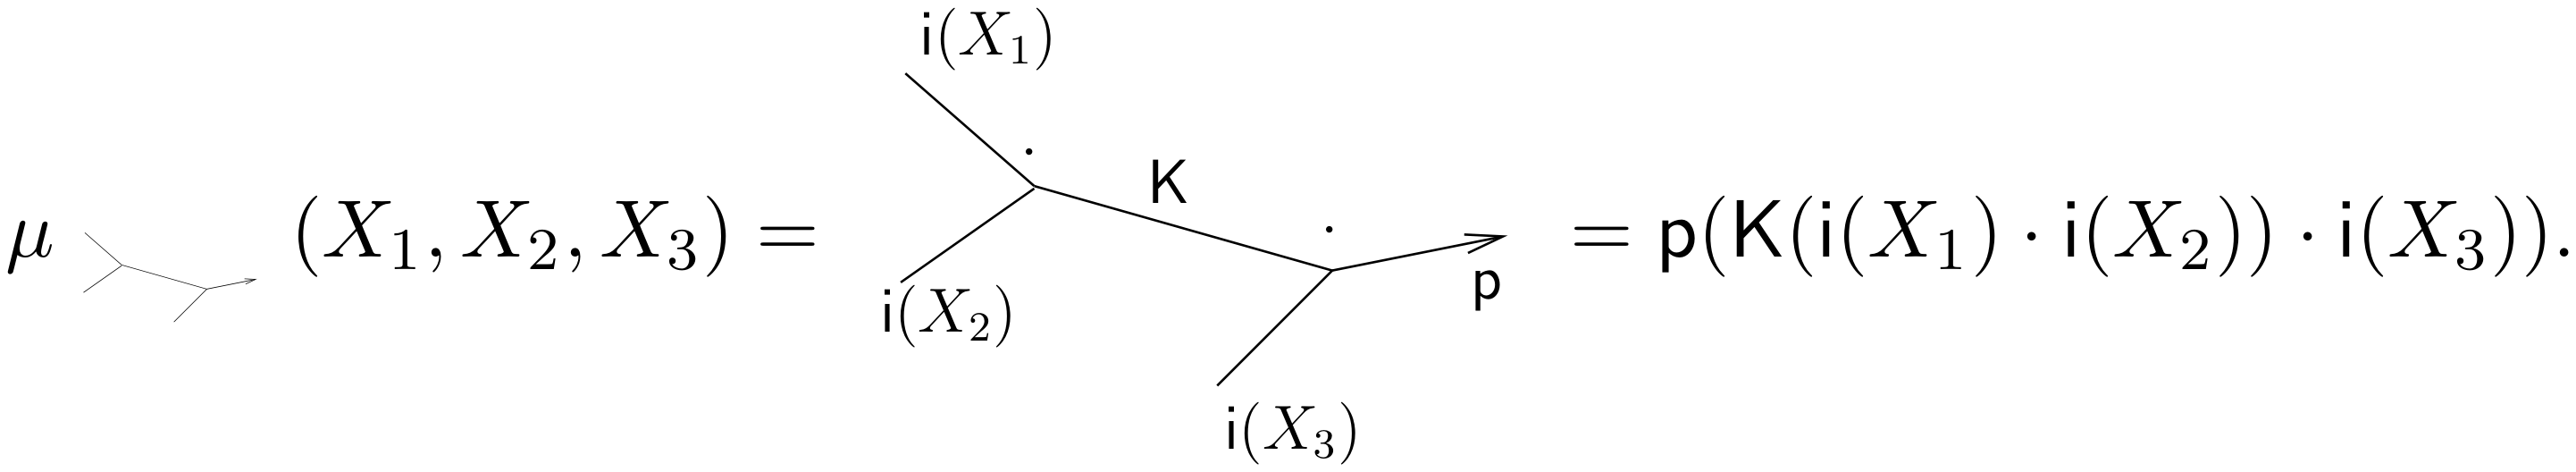
\includegraphics[width=0.86\linewidth]{figtree33.png}
\end{center}
% 上式在源码中的可编辑形式（供检索与改写；排版时由上面原图代替）：
% \mu(X_1,X_2,X_3)=\mathrm{p}\bigl(K(\mathrm{i}(X_1)\cdot \mathrm{i}(X_2))\cdot \mathrm{i}(X_3)\bigr).
\end{itemize}

% [Tutor Note: 次数核对：$n$ 叶二叉有根树有 $n-1$ 个内部顶点、$n-2$ 条内部边；乘积次数为 $0$，$K$ 的次数为 $-1$，故 $\mu_n$ 的次数为 $2-n$，与式~\eqref{eq:3} 中复合映射的次数一致。若把 $K$ 与乘积的次数记反，式~\eqref{eq:36} 的符号会整体错位。]
% [Tutor Note: 上式原书是手绘的二叉树（叶装饰 $\mathrm{i}(X_1),\mathrm{i}(X_2),\mathrm{i}(X_3)$，先由乘积合并前两个叶，在内部边上作用 $K$ 后再与第三个叶相乘，最后在根处作用 $\mathrm{p}$）。译文按原式整行裁图插入（图文件 \mbox{figtree33.png}），未重排；其组合型由「$n$ 叶二叉有根树」与上面的装饰规则唯一决定。]

这个诱导出的 $\mathbb{M}$ 上的 $\Ainf$ 代数结构与 $\Ainf$ 范畴 $\mathbb{F}$ 的关系如下。设给定一列可复合的态射
\begin{equation}\tag{34}\label{eq:34}
F_{a_1}\xrightarrow{x_1}F_{a_2}\xrightarrow{x_2}\cdots\xrightarrow{x_n}F_{a_{n+1}},
\end{equation}
其中当 $a_i\neq a_{i+1}$ 时，$x_i$ 是 $F_{a_i}-F_{a_{i+1}}$ 的临界点（更一般地，是 Morse 链）；当 $a_i=a_{i+1}$ 时，$x_i$ 是一条链。则
\begin{equation}\tag{35}\label{eq:35}
m(x_1,\dots,x_n)=\mu(X_1,\dots,X_n).
\end{equation}
左边是范畴 $\mathbb{F}$ 中的复合，右边是代数 $\mathbb{M}$ 中的高阶乘法。右边的输入取为：当 $a_i\neq a_{i+1}$ 时 $X_i=x_i$；当 $a_i=a_{i+1}$ 时 $X_i=\delta^{\epsilon}_{x_i}$，即链 $x_i$ 的 $\epsilon$-光滑化 delta 形式。我们把每个输入 $X_i$ 都理解为 $\mathbb{M}_{a_ia_{i+1}}$ 中的一个元素。等式~\eqref{eq:35} 对充分小的正规化参数 $\epsilon$ 成立，\footnote{不能为 $\mathbb{F}$ 中所有复合统一选取“充分小”的 $\epsilon$：$\epsilon$ 的界依赖于式~\eqref{eq:35} 中的输入链。归根结底，这是因为式~\eqref{eq:18} 中 $\epsilon$ 的界依赖于输入链。}并且由比较式~\eqref{eq:33} 与式~\eqref{eq:31}、式~\eqref{eq:4} 得到。\footnote{为完整起见我们指出，还有式~\eqref{eq:34} 中首、末对象重合的特殊情形，即 $a_1=a_{n+1}$。此时 $m(x_1,\dots,x_n)$ 是一条链（见第~\ref{sec:2.1} 节定理~\ref{thm:1} 之前的讨论），而 $\mu(X_1,\dots,X_n)$ 是该链的 $\epsilon$-光滑化 delta 形式。}

% [Tutor Note: $X_i$ 落在哪个分块极易记错：$a_i\neq a_{i+1}$ 时 $X_i=x_i$ 是 $\mathbb{M}_{a_ia_{i+1}}=\mathrm{MC}(F_{a_i}-F_{a_{i+1}})$ 中的临界点或 Morse 链；$a_i=a_{i+1}$ 时 $X_i=\delta^{\epsilon}_{x_i}$ 落在 $\Omega_{a_ia_i}$ 中。$\delta^{\epsilon}_{x_i}$ 不是临界点，必须当作光滑化 delta 形式才能进入树形公式~\eqref{eq:33}。]

\begin{thmenv}{注}{3.1}\label{rem:3.1}
在式~\eqref{eq:35} 中，Kontsevich--Soibelman 公式~\eqref{eq:33} 里一棵二叉有根树 $T$ 的贡献，对应式~\eqref{eq:31} 中一棵允许 2 价顶点的有根树 $T'$ 的贡献。这里 $T'$ 由 $T$ 去掉这样的 1 价顶点及其相邻边得到：该顶点的输入落在 $\mathbb{M}_{a_ia_{i+1}}$ 中，且 $a_i=a_{i+1}$。每一次这样的去除，都在 $T'$ 中生成一个 2 价顶点。
\end{thmenv}

% [Tutor Note: 这一步是式~\eqref{eq:33} 与式~\eqref{eq:31} 逐项对应的组合核心。式~\eqref{eq:31} 的树允许 2 价顶点来承载链 $Z_{\alpha,a}$；而式~\eqref{eq:33} 的二叉树叶在 $a_i=a_{i+1}$ 时带的是 $\delta^{\epsilon}_{x_i}$。截去这样的叶及其边，相当于把它并进 $\delta_{Z}$ 型因子，同时在 $T'$ 中留出一个 2 价顶点。图~\ref{fig:8} 给出的正是最简单的例子。]

\begin{figure}[htbp]
  \centering
  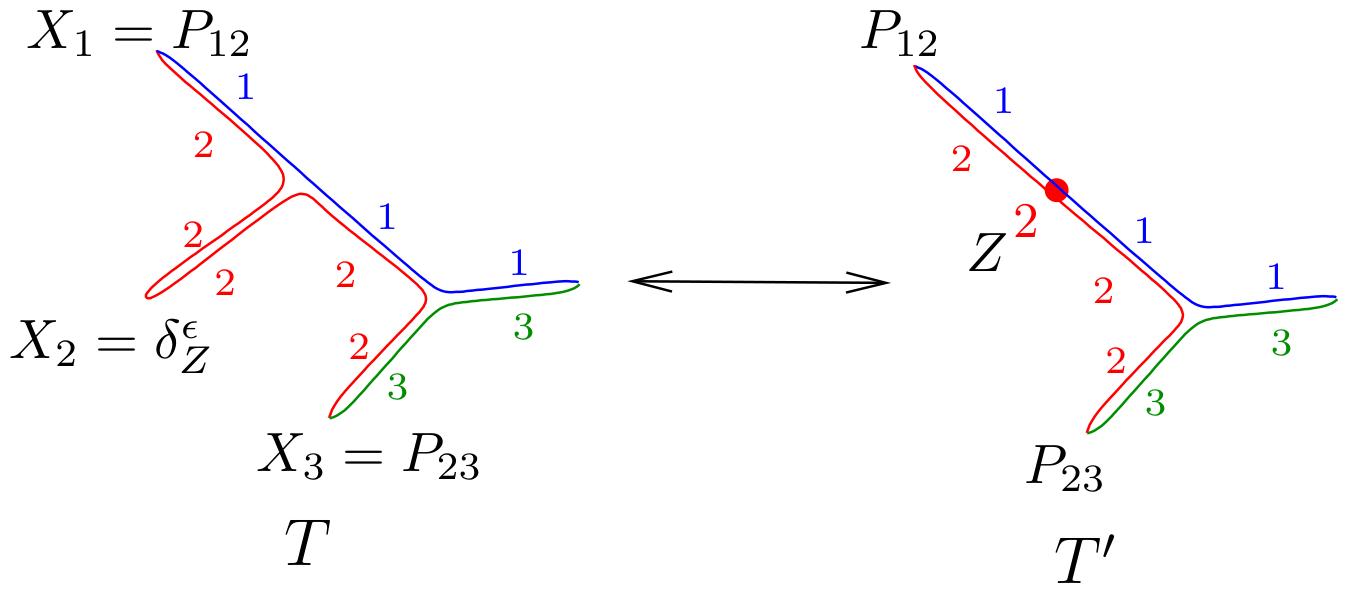
\includegraphics[width=\linewidth]{fig08.png}
  \caption{例：一个贡献到式~\eqref{eq:31} 的非二叉树，它由贡献到 Kontsevich--Soibelman 同伦转移公式的一个二叉树截去一个 $(aa)$-叶（图中 $a=2$）得到。图中明确标出了各边的双色。（原书 p.16）}
  \label{fig:8}
\end{figure}

由 Kontsevich--Soibleman 的一般结果 \cite{kontsevichsoibelman}，$\mathbb{M}$ 上诱导的高阶乘法 $\mu$ 满足 $\Ainf$ 代数关系式：
\begin{equation}\tag{36}\label{eq:36}
\sum_{r\ge0,\ s\ge1,\ r+s\le n}
\pm\,\mu\bigl(X_1,\dots,X_r,\ \mu(X_{r+1},\dots,X_{r+s}),\ X_{r+s+1},\dots,X_n\bigr)=0
\end{equation}
对任意输入 $X_1,\dots,X_n\in\mathbb{M}$ 成立。由式~\eqref{eq:35}，这蕴含 $\mathbb{F}$ 中复合映射的 $\Ainf$ 范畴关系式~\eqref{eq:7}。

% [Tutor Note: 原书 p.17 把 Soibelman 拼作 Soibleman，疑为笔误；译文照录，未擅改。读者应把它与 \cite{kontsevichsoibelman} 中的 Soibelman 认作同一人，切勿当成另一文献。]

\subsection{用 BF 理论有效作用量的进路}\label{sec:3.2}

\begin{takeaway}
\begin{itemize}
  \item \textbf{物理图像}：把上面的证明理解为 BF 理论的二次量子化：先写出 BV 形式下的 BF 作用量，再对非对角（快）场作纤维 BV 积分，得到只含对角慢场的有效作用量。
  \item \textbf{数学工具}：Batalin--Vilkovisky 形式、上三角矩阵代数 $\mathcal A$ 的正向极限、Nekrasov 型非对角轴规范、奇辛纤维化、Feynman 图展开。
  \item \textbf{主要结论}：有效作用量是 Feynman 树之和~\eqref{eq:41}，式~\eqref{eq:42} 给出前几项；BV 主方程~\eqref{eq:45} 等价于 $L_\infty$ 关系式~\eqref{eq:46}，再由式~\eqref{eq:47} 恢复 $\Ainf$ 乘法 $\mu_n$。
\end{itemize}
\end{takeaway}

上面所用的物理证明，可以用“二次量子化”来解释。也就是说，我们考虑 Batalin--Vilkovisky 形式下的 BF 理论\footnote{BV 形式下以非齐次微分形式为场的非阿贝尔 BF 理论，参看 \cite{cattaneo}。}，它由作用量
\begin{equation}\tag{37}\label{eq:37}
S=\int_X\Bigl\langle B,\ dA+\frac12[A,A]\Bigr\rangle
\end{equation}
定义。其中场 $A$ 是取值于李代数 $\mathfrak g=\mathfrak{gl}_N(\mathcal A)$ 的微分形式。这里 $\mathfrak g$ 是元素取自 $\mathcal A$ 的 $N\times N$ 矩阵构成的李代数；$\mathcal A$ 是 $\widetilde N\times\widetilde N$ 的上三角矩阵代数，其中 $\widetilde N$ 很大（更确切地说，我们取正向极限 $\widetilde N\to\infty$）。$B$ 是取值于 $\mathfrak g^*$ 的微分形式。

% [Tutor Note: 式~\eqref{eq:37} 有三层结构：$A$ 的矩阵指标在 $N\times N$ 上（对应 $\mathbb{F}$ 的 $N$ 个对象），每个矩阵元再取值于 $\mathcal A$（大型上三角矩阵代数）。$\langle\,,\rangle$ 是 $\mathfrak g$ 与 $\mathfrak g^*$ 的配对；对微分形式还要配上 wedge 积与矩阵迹，原文按标准 BF 记号省略未写。$A$ 是奇变量，故 $dA+\frac12[A,A]$ 就是曲率。]

\begin{thmenv}{注}{3.2}\label{rem:3.2}
若只考虑以 $N\times N$ 矩阵为系数的 BF 理论，那么通过有效作用量得到的将是 $\mathbb{M}$ 上的 $L_\infty$ 代数结构，即所需 $\Ainf$ 结构的反对称化。于是，用这样的系数会丢掉高阶乘法的一部分数据。为弥补这一点，我们让场的 $(a,b)$-分量取值于 $\mathcal A$，由此引入非交换性。这相当于先把 $\Ainf$ 代数 $\mathbb{M}$ 与 $\mathcal A$ 作张量积，再做反对称化。所得的 $\mathbb{M}\otimes\mathcal A$ 上的 $L_\infty$ 括号，能记住 $\mathbb{M}$ 上 arity 至多 $\widetilde N-1$ 的 $\Ainf$ 乘法 $\mu$，见下文式~\eqref{eq:47}。
\end{thmenv}

% [Tutor Note: 为何必须把系数扩成 $\mathcal A$：只取 $N\times N$ 矩阵时，反对称化后只能读到 $L_\infty$ 括号，$\Ainf$ 的 $\mu_n$ 被混同。张量 $\mathcal A$ 之后，矩阵单位 $t_{ij}$ 像「标签」一样把输入与输出的次序记下来（见式~\eqref{eq:47}）。再取正向极限 $\widetilde N\to\infty$，是为了不设 arity 的上限。$\mathcal A$ 幂零这一点，在「非幂零 $\mathfrak g$」那条脚注处会用到。]

我们把 $A$ 分解为对角场 $A_Z$（相对于 $M_N$ 因子）与非对角场 $A_W$。名称来自标准模型中的 $Z$、$W$ 规范玻色子。然后我们采用一个精巧版本的规范固定，它推广了轴规范（最早由 N.~Nekrasov 在与 A.~Losev 的私人通信中提出）：\footnote{注意通常的轴（或时间）规范是 $A_0=0$，即 $\iota_{\frac{\partial}{\partial t}}A=0$。这里推广的一个特点是：我们对规范场的不同分量取不同的向量场。}
\begin{equation}\tag{38}\label{eq:38}
\iota_{v_{ab}}(A_W)_{ab}=0,
\end{equation}
其中 $v_{ab}$ 是 $F_a-F_b$ 的梯度向量场。我们指出，这个规范条件等价于 Morse 链同伦式~\eqref{eq:12} 把 $(A_W)_{ab}$ 湮灭。

% [Tutor Note: 式~\eqref{eq:38} 把「几何」塞进了规范固定：$\iota_{v_{ab}}$ 是沿梯度场 $v_{ab}$ 的缩并。作者断言这个条件等价于「$(A_W)_{ab}$ 被 Morse 链同伦式~\eqref{eq:12} 湮灭」。结合下文 $\mathcal L=\mathrm{im}K\oplus\mathrm{im}K$，这条等价关系正是「几何规范固定转化为内部边装饰 $K$」的翻译词典，也是全节物理思想的关键一步。]

经过这样的规范固定，我们直接把场 $A_W$ 积掉，就得到只含 $A_Z$ 场与临界点的有效理论，而临界点是 $A_W$ 场的残余。

\textbf{更多细节.}\quad 有效作用量由纤维 BV 积分定义：
\begin{equation}\tag{39}\label{eq:39}
e^{\frac{i}{\hbar}S_{\mathrm{eff}}(A',B')}=\int_{\mathcal L}e^{\frac{i}{\hbar}S(A,B)},
\end{equation}
积分沿奇辛纤维化
\begin{equation}\tag{40}\label{eq:40}
\Omega^\bullet(X,\mathfrak g)[1]\oplus\Omega^\bullet(X,\mathfrak g^*)[\dim X-2]
\ \longrightarrow\
\mathbb{M}\otimes\mathcal A[1]\oplus\mathbb{M}\otimes\mathcal A^*[\dim X-2]
\end{equation}
的纤维中的一个 Lagrangian $\mathcal L$ 进行。左边是 BF 理论的 BV 场空间（其元素为对 $(A,B)$），右边是我们选定的“慢场”空间，其元素记作 $(A',B')$。式~\eqref{eq:40} 中的投影是 $\mathrm{p}\oplus\mathrm{p}$，由式~\eqref{eq:32} 的映射拼成，并按 $\mathcal A$-线性延拓；它也有截面 $\mathrm{i}\oplus\mathrm{i}$。式~\eqref{eq:40} 纤维中的 Lagrangian $\mathcal L$ 由规范固定条件~\eqref{eq:38} 确定，换言之由 $\mathcal L=\mathrm{im}K\oplus\mathrm{im}K$ 给出。

% [Tutor Note: 式~\eqref{eq:40} 两端的方括号是次数平移：$[1]$ 与 $[\dim X-2]$ 必须逐项对齐，混淆两者会破坏奇辛配对的次数。右端 $\mathbb{M}\otimes\mathcal A^*$ 中的星号是对 $\mathcal A$ 取对偶，不是对整个张量积取对偶。$\mathcal L=\mathrm{im}K\oplus\mathrm{im}K$ 说明纤维积分沿 $K$ 的像进行，故内部边最终由 $K$ 装饰。]

把纤维 BV 积分~\eqref{eq:39} 当作受扰高斯积分算出来，有效作用量就写成 Feynman 图之和：
\begin{equation}\tag{41}\label{eq:41}
S_{\mathrm{eff}}=\sum_{\Gamma}\frac{1}{|\mathrm{Aut}(\Gamma)|}\Phi_\Gamma(A',B').
\end{equation}
这里
\begin{itemize}
  \item 求和取遍二叉有根树 $\Gamma$（Feynman 图），按图同构类计。
  \item $|\mathrm{Aut}(\Gamma)|$ 是树 $\Gamma$ 的自同构群的阶。
  \item $\Phi_\Gamma(A',B')$ 是慢场空间（式~\eqref{eq:40} 的右端）上的多项式函数。它的做法是：用 $\mathrm{i}(A')$ 装饰 $\Gamma$ 的叶，用 $\langle B',\mathrm{p}(\cdots)\rangle$ 装饰根，用 dg 李代数 $\Omega^\bullet(X,\mathfrak g)$ 中的李括号装饰二叉顶点，用链同伦 $K$ 装饰内部边。
\end{itemize}

式~\eqref{eq:41} 的前几项是：
\begin{equation}\tag{42}\label{eq:42}
\begin{split}
S_{\mathrm{eff}}={}&
\langle B',d_{\mathbb{M}}A'\rangle
+\frac12\langle B',\mathrm{p}[\mathrm{i}(A'),\mathrm{i}(A')]\rangle
+\frac12\langle B',\mathrm{p}[K[\mathrm{i}(A'),\mathrm{i}(A')],\mathrm{i}(A')]\rangle\\
&+\frac12\langle B',\mathrm{p}[K[K[\mathrm{i}(A'),\mathrm{i}(A')],\mathrm{i}(A')],\mathrm{i}(A')]\rangle
+\frac18\langle B',[K[\mathrm{i}(A'),\mathrm{i}(A')],K[\mathrm{i}(A'),\mathrm{i}(A')]]\rangle+\cdots
\end{split}
\end{equation}

% [Tutor Note: 系数与 $|\mathrm{Aut}(\Gamma)|$ 对应：前三个单链树的权重是 $1/2$；最后的「哑铃」树两条 $K$ 边可交换，自同构群阶为 $8$，故系数是 $1/8$ 而不是 $1/4$。抄写式~\eqref{eq:42} 时最易在此出错，请对原书 p.18 第二行逐字核对。]

\textbf{用对角场与非对角场来描述.}\quad 可以把场（以及慢场）相对于 $M_N$ 因子分成对角分量与非对角分量：
\[
\begin{gathered}
A=A_Z+A_W,\qquad B=B_Z+B_W,\\
A'=A_Z+A'_W,\qquad B'=B_Z+B'_W.
\end{gathered}
\]
于是作用量~\eqref{eq:37} 成为
\begin{equation}\tag{43}\label{eq:43}
\begin{split}
S=\int_X&\,\underset{(a)}{\langle B_Z,dA_Z\rangle}
+\underset{(b)}{\langle B_W,dA_W\rangle}
+\underset{(c)}{\Bigl\langle B_W,\frac12[A_W,A_W]\Bigr\rangle}\\
&+\underset{(d)}{\langle B_W,[A_Z,A_W]\rangle}
+\underset{(e)}{\Bigl\langle B_Z,\frac12[A_Z,A_Z]\Bigr\rangle}
+\underset{(f)}{\Bigl\langle B_Z,\frac12[A_W,A_W]\Bigr\rangle}.
\end{split}
\end{equation}
场 $A_Z,B_Z$ 是非动力学的：在式~\eqref{eq:39} 中不对它们积分；而 $A_W,B_W$ 是动力学场。在式~\eqref{eq:43} 中：
\begin{itemize}
  \item 项 (a)、(e) 是常数。
  \item (b) 是动力学场的动能项，它产生分配给各条边的“传播子”$K$。
  \item (c) 产生一个三价“相互作用”顶点（两条入半边与一条出半边）。
  \item (d) 产生一个三价顶点，带一条自由的（或“外部的”）入半边，其装饰为 $A_Z$。
  \item (f) 产生一个三价顶点，带一条自由的出半边，其装饰为 $B_Z$。
  \item 带 $A_W$ 的半边既可以是外部的（装饰为 $A'_W$），也可以是内部的（对应于该场分量的快部分、即动力学部分）。内部半边与一条内部的 $B_W$ 半边相连，所得的内部边由传播子装饰。类似地，$B_W$ 半边可以是外部的，也可以是内部的。
\end{itemize}

% [Tutor Note: 六项分工要记清：(b)(c) 只含 $A_W$，给出传播子与三价相互作用；(a)(e) 不含 $A_W$，在纤维积分中是常数；(d)(f) 各带一条 $A_Z$ 或 $B_Z$ 的外线，把慢场接到动力学部分。注意 (e) 与 (f) 的被积式都含 $\frac12[\cdot,\cdot]$，但 (e) 是常数项、(f) 是外线顶角，切勿记反。]

\begin{figure}[htbp]
  \centering
  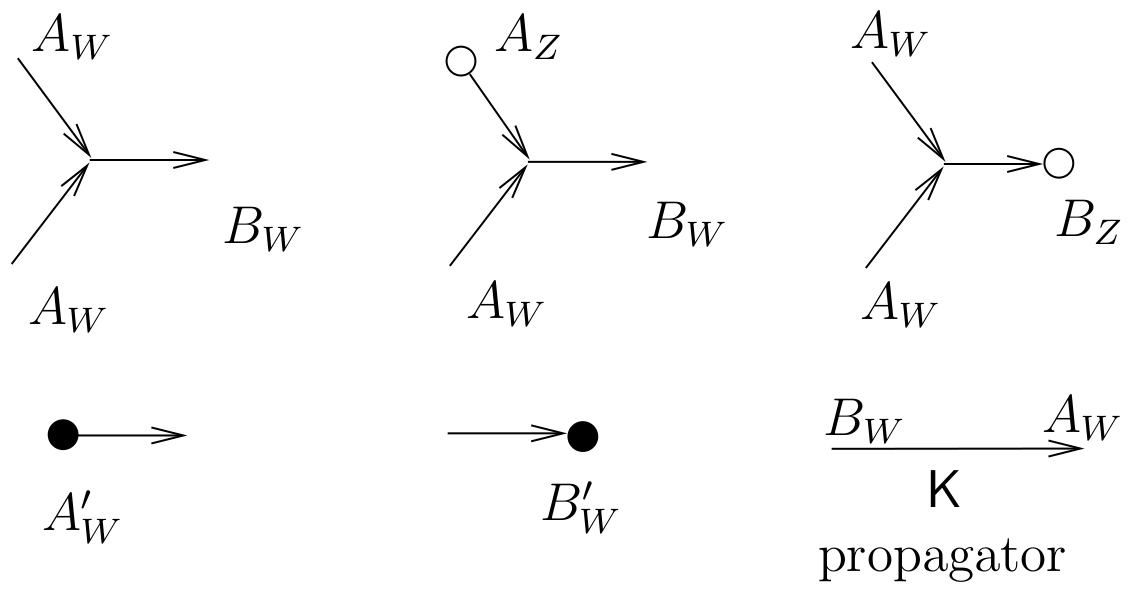
\includegraphics[width=0.9\linewidth]{fig09.png}
  \caption{Feynman 规则（Feynman 图的构件）。（原书 p.19）}
  \label{fig:9}
\end{figure}

\begin{figure}[htbp]
  \centering
  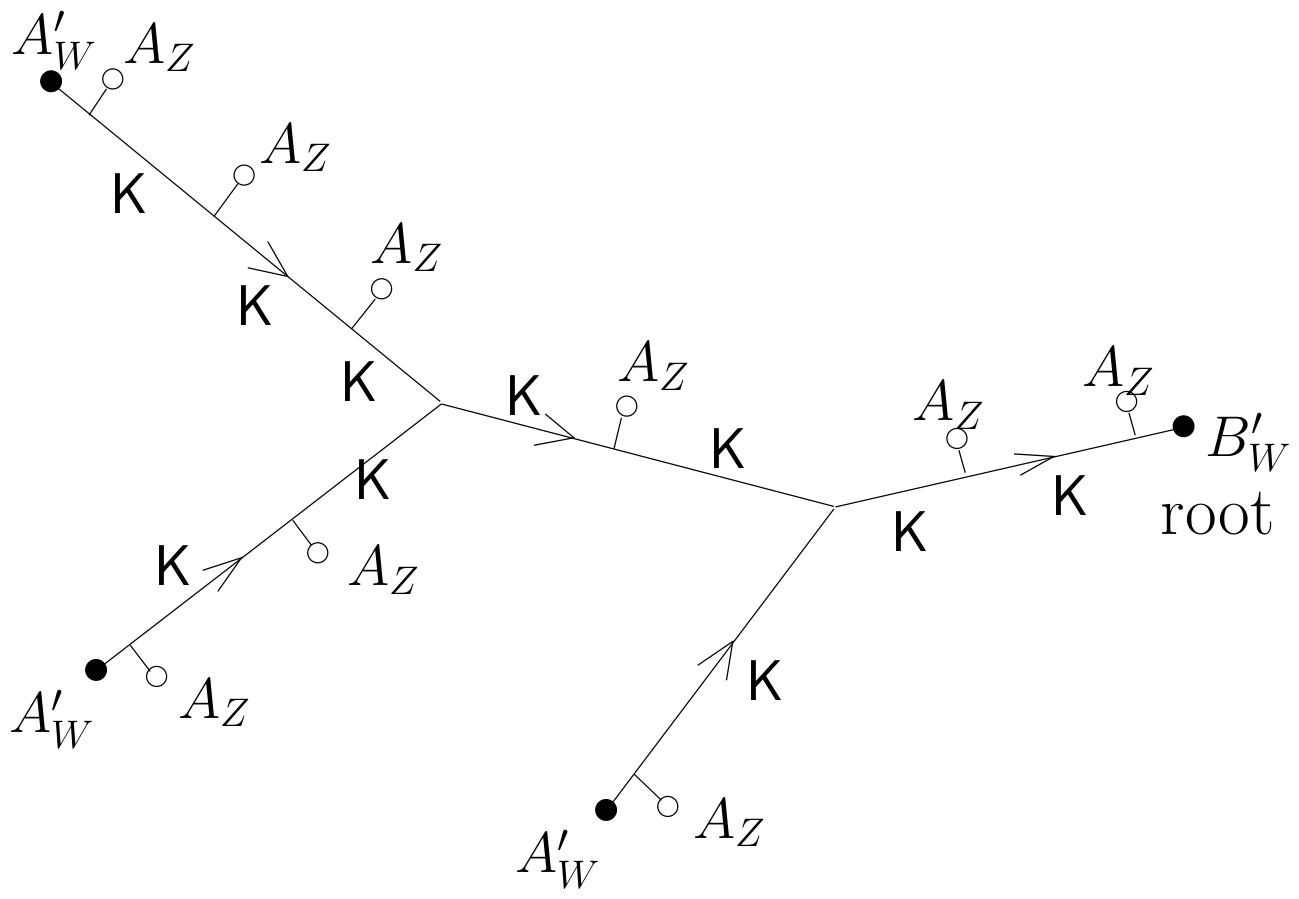
\includegraphics[width=0.9\linewidth]{fig10.png}
  \caption{一个贡献到 $S_{\mathrm{eff}}$ 的典型 Feynman 树，图中明确画出了场的对角部分与非对角部分。（原书 p.19）}
  \label{fig:10}
\end{figure}

把叶数相同的 Feynman 树的贡献归并起来，可以把 $S_{\mathrm{eff}}$ 写成
\begin{equation}\tag{44}\label{eq:44}
S_{\mathrm{eff}}=\sum_{n\ge1}\frac{1}{n!}\langle B',l_n(A',\dots,A')\rangle,
\end{equation}
其中 $l_n\colon\wedge^n(\mathbb{M}\otimes\mathcal A)\to\mathbb{M}\otimes\mathcal A$ 是由 $n$ 叶 Feynman 树给出的斜对称多线性运算。按 Feynman 图展开~\eqref{eq:41}，$l_n$ 可以写成非平面（或按同构类计的）二叉有根树之和，这是 Kontsevich--Soibelman 公式~\eqref{eq:33} 的李代数版本。我们指出，虽然一般地 BF 理论的有效作用量含有单圈图，但在我们这里它们消失，因为系数李代数 $\mathfrak g$ 幂零。\footnote{事实上，考虑非幂零的 $\mathfrak g$ 是很有意思的。例如取 $\mathcal A$ 为所有 $\widetilde N\times\widetilde N$ 矩阵的代数，这样有效作用量中会出现非平凡的单圈图。把它们理解为 Fukaya--Morse 范畴的“圈增强”，是作者们正在进行的工作。}

% [Tutor Note: $1/n!$ 来自 $n$ 个等价输入 $A'$ 的置换（$l_n$ 斜对称，$n!$ 个置换给出同一项）。按叶数归并式~\eqref{eq:41} 时，这个因子必须与树的同构群阶数一起核对，否则会差整数倍。]

我们要强调：按规范理论的逻辑，我们在为快场（慢场的补）上的积分~\eqref{eq:39} 选取规范固定。在 BV 形式中，这相当于在快场中选一个 Lagrangian 子空间；把积分改写成 Feynman 图之和时，这个子空间就对应传播子（即对边的装饰）。于是，我们的几何规范固定对应于“边被 Morse 链同伦式~\eqref{eq:12} 装饰”，而这又使得（在此规范下算出的）有效作用量与 Morse 树的计数相关。

% [Tutor Note: 这一段是全节的物理枢纽，值得慢读：规范固定（几何条件）→ 传播子（Feynman 规则里的边装饰）→ Morse 链同伦 $K$（组合数据）→ Morse 树计数（范畴的复合）。四个对象其实是同一件事的四种语言，作者用「规范理论的逻辑」把它们串成一条链。若省略这一步，读者会误以为 BF 有效作用量与 Morse 树计数只是碰巧形式相似。]

作用量~\eqref{eq:37} 满足 BV 主方程 $\{S,S\}=0$，这是 $\mathfrak g$-值形式的 dg 李代数中二次关系式 $d^2=0$、Leibniz 法则与 Jacobi 恒等式的推论。这里 $\{\,,\}$ 是与场空间上奇辛形式相伴的 Poisson 括号。因此，由纤维 BV 积分的 BV--Stokes 定理，有效作用量也满足主方程
\begin{equation}\tag{45}\label{eq:45}
\{S_{\mathrm{eff}},S_{\mathrm{eff}}\}=0.
\end{equation}
它等价于运算 $l_n$ 上的 $L_\infty$ 代数二次关系式：
\begin{equation}\tag{46}\label{eq:46}
\sum_{r\ge0,\ s\ge1,\ r+s=n}\frac{1}{r!\,s!}\sum_{\sigma\in S_n}
\pm\,l_{r+1}\bigl(y_{\sigma(1)},\dots,y_{\sigma(r)},l_s(y_{\sigma(r+1)},\dots,y_{\sigma(n)})\bigr)=0,
\end{equation}
其中 $y_1,\dots,y_n\in\mathbb{M}\otimes\mathcal A$ 是输入，$\sigma$ 取遍置换。关于通过纤维 BV 积分作 $L_\infty$ 代数的同伦转移，读者可参看 \cite{mnev}。

% [Tutor Note: 式~\eqref{eq:46} 与式~\eqref{eq:36} 的求和范围不同：这里 $r+s=n$，$n$ 个输入由置换 $\sigma$ 分配进内外两个括号，全部参与；而 $\Ainf$ 的式~\eqref{eq:36} 允许 $r+s\le n$，尾部可有剩余输入。照抄式~\eqref{eq:36} 的范围会漏项。]

\textbf{从 $L_\infty$ 回到 $\Ainf$.}\quad 我们可以从 $L_\infty$ 括号 $l_n$ 恢复 $\mathbb{M}$ 中的 $\Ainf$ 乘法（从而恢复 $\mathbb{F}$ 中的高阶复合）如下：
\begin{equation}\tag{47}\label{eq:47}
l_n(X_1\otimes t_{12},\dots,X_n\otimes t_{n,n+1})=\mu_n(X_1,\dots,X_n)\otimes t_{1,n+1},
\end{equation}
其中 $t_{ij}\in\mathcal A$ 是在 $(i,j)$ 位置为 $1$、其余元素为零的矩阵。这里 $X_i$ 是 $\mathbb{M}_{a_ib_i}$ 中的元素，我们要求 $b_i=a_{i+1}$（否则式~\eqref{eq:47} 两端都为零）。

% [Tutor Note: $t_{ij}$ 是上三角矩阵代数 $\mathcal A$ 中的矩阵单位。取 $t_{12},t_{23},\dots,t_{n,n+1}$ 是沿态射链 $(a_1,a_2),\dots,(a_n,a_{n+1})$ 把指标串起来，输出恰好落在 $t_{1,n+1}$ 上。若 $b_i\neq a_{i+1}$，乘积在 $\mathcal A$ 中为零，式~\eqref{eq:47} 两端同时消失。这正是 $\mathcal A$ 能「记住」$\Ainf$ 复合的组合机制。]
\endinput

% =====================================================================
%  第 4 节  用一次量子化证明 A∞ 关系式（原书 p.20–25）
%  含 4.1、4.2、式 (48)–(56)、例 6、例 7、注 4.1、图 11、图 12
% =====================================================================
\section{用一次量子化证明 $\Ainf$ 关系式}\label{sec:4}

\begin{takeaway}
\begin{itemize}
  \item \textbf{物理图像}：把 $X$ 上单粒子的超量子力学放到树上。每条边是一段“时间”，超传播子 $U(t,\mathrm{d}t)=e^{-tH-\mathrm{d}t\,G}$ 沿边传播态；叶子是入态（$F_a-F_b$ 的 Lefschetz thimble 上的 delta 形式），2 价顶点是“乘以链 $Z$ 上 delta 形式”的插入算子，3 价顶点按 $(a,b)\times(b,c)=(a,c)$ 把颜色接起来。
  \item \textbf{数学工具}：度量树模空间 $MT_{a_1,\dots,a_r;k_1,\dots,k_r}$；取值于 $\mathrm{Hom}$ 空间的微分形式 $I$；Morse 收缩的三元组 $(i,p,K)$ 与超传播子在边趋于无穷时的行为 $U(+\infty)=i\circ p$；模空间上的 Stokes 定理。
  \item \textbf{主要结论}：$I$ 满足 $(\mathrm{d}_{MT}+Q)I=0$，在红外边界上分解，其周期恰为复合映射 $m$。把这条闭性等式在模空间上积分，两端分别给出 $Qm$ 与边界层片之和；五类层片中三类相消、两类保留，合起来正是 $A_\infty$ 关系式~\eqref{eq:7}。
\end{itemize}
\end{takeaway}

% [Tutor Note: 本节是第~\ref{sec:3} 节的“对偶”版本。第~\ref{sec:3} 节走二次量子化：把 $X$ 上的 BF 理论作纤维 BV 积分，树是 Feynman 图。本节走一次量子化：树本身是单粒子超量子力学的“时间轴分叉”，模空间 $MT$ 只负责记录各边长度。两条路线给出同一批复合映射，但本节只需 $MT$ 上一个闭形式加 Stokes 定理。]

\subsection{树上高阶拓扑量子力学的进路：思路}\label{sec:4.1}

\begin{takeaway}
\begin{itemize}
  \item \textbf{物理图像}：单粒子的超量子力学以 $Q=\mathrm{d}$ 为奇幂零对称性，取 $G=\iota_{v_{ab}}$、$H=[Q,G]=L_{v_{ab}}$：$G$ 降一次、$H$ 保持次数。树的分叉由 3 价顶点按颜色规则实现，叶子与链则作为入态或插入算子。
  \item \textbf{数学工具}：类型为 $(a,b)$ 的粒子、态空间 $\Omega^\bullet(X)$、超传播子 $U(t,\mathrm{d}t)$、带度量且顶点价数为 1、2、3 的树。
  \item \textbf{主要结论}：由 $U$ 的展开得到边长度空间上的闭微分形式；它在某条边趋于无穷时分解。于是沿红外边界积分，就得到 $A_\infty$ 关系式的粗略论证；细节见第~\ref{sec:4.2} 节。
\end{itemize}
\end{takeaway}

我们考虑树上的高阶拓扑量子力学，给出范畴 $\mathbb{F}$ 中 $A_\infty$ 关系式~\eqref{eq:7} 的第二个证明。\footnote{高阶拓扑量子力学（higher topological quantum mechanics，HTQM）的设定见 \cite{losev,losevpolyubin}。粗略地说，HTQM 就是度量树模空间上的一个闭微分形式，它在任何一条边变得无限长时分解。于是由模空间上的 Stokes 定理，该形式的各个周期之间出现二次关系。这套框架本质上是一个链层面、一维的上同调场论，见 \cite{kontsevichmanin}。}

普通量子力学由粒子的态空间与 Hamilton 量描述。我们考虑类型为 $(a,b)$（$a\neq b$）的粒子，其态空间始终取流形 $X$ 上微分形式构成的空间。Hamilton 量取为沿 $F_a-F_b$ 的梯度向量场 $v_{ab}$ 的 Lie 导数 $L_{v_{ab}}$。这类 Hamilton 量关于一个奇、幂零的对称性 $Q$ 是正合的：
\[
  Q=\mathrm{d},\qquad G=\iota_{v_{ab}},\qquad H=[Q,G]=L_{v_{ab}}.
\]

我们考虑带度量（即各边长度）的树，其顶点的价数为 1、2、3。

1 价顶点是一个态：对 $(a,b)$-粒子，我们把这个态取为函数 $F_a-F_b$ 的临界点 $P_{ab}$ 所对应的 Lefschetz thimble（不稳定流形）上的 delta 形式。2 价顶点不过是态空间中的一个算子，即乘以链 $Z$ 上 delta 形式的算子。3 价顶点是微分形式的乘法，并配上规则
\[
  (a,b)\times(b,c)=(a,c),
\]
其余情形取零。我们用超传播子（又称演化算子）
\begin{equation}\tag{48}\label{eq:48}
  U(t,\mathrm{d}t)=\exp(-tH-\mathrm{d}t\,G)
\end{equation}
来构造边长度空间上的微分形式。这个对象已在上文讨论 Morse 收缩时出现过，见式~\eqref{eq:9}。

% [Tutor Note: 式 (48) 与式 (9) 是同一个算子：式 (9) 把它写成 $e^{-tL_v}(1-\mathrm{d}t\,\iota_v)$。因为 $(\mathrm{d}t\,\iota_v)^2=0$ 且 $[L_v,\iota_v]=0$，指数可以拆开，两种写法一致。关键在于每次出现 $\mathrm{d}t$ 必同时出现一个 $\iota_v$，这条“捆绑”是全节次数计数的起点。]

把该传播子展开，就得到边长度空间上的一个微分形式。当某条边的长度趋于无穷时，这个形式分解。

论证的粗略思路如下（正确的版本见下文）。按上述方式构造的微分形式是闭的。因此可以沿红外边界（即某条边的长度等于无穷时）对它积分。利用分解性质，就得到各长度空间上的积分之间所期望的二次关系，而这些关系恰是我们要证明的 $A_\infty$ 关系式~\eqref{eq:7}。

% [Tutor Note: 这条“闭形式加边界分解”的论证与上同调场论中 WDVV 方程的证明同构：那里模空间是带四个标记点的球面模空间（复一维），边界是三个点；这里模空间是一维的树模空间，边界只由 $t\to0$ 与 $t\to+\infty$ 组成。两者都归结为一组二次关系，一维版本就是 $\Ainf$ 关系式。见 \cite{losev,kontsevichmanin}。]

\subsection{更多细节}\label{sec:4.2}

\begin{takeaway}
\begin{itemize}
  \item \textbf{物理图像}：一个胞腔由树的组合型与各内部边长 $t,t',t''$ 的正实数值决定；边长为零等于把该边收缩，边长趋于无穷则是红外边界。$I$ 是把 $U$ 逐边装配、再在 2 价顶点插入链得到的微分形式。
  \item \textbf{数学工具}：$MT_{a_1,\dots,a_r;k_1,\dots,k_r}$、形式 $I$ 及其三条性质（闭性、红外分解、周期）、式~\eqref{eq:14} 的 $(\mathrm{d}_t+Q)$-闭性、$\mathrm{d}t$-次数计数。
  \item \textbf{主要结论}：由 $(\mathrm{d}_{MT}+Q)I=0$ 与 Stokes 定理得式~\eqref{eq:55}；左端按边界层片分成五类，(a)(b)(c) 三类两两相消，(d)(e) 两类保留，与右端的 $Qm$ 合起来正好是 $A_\infty$ 关系式。例~\ref{ex:7} 与图~\ref{fig:12} 给出具体核对。
\end{itemize}
\end{takeaway}

固定一列“颜色” $a_1,\dots,a_r\in\{1,\dots,N\}$，满足对一切 $i$ 有 $a_i\neq a_{i+1}$；再固定一列整数 $k_1,\dots,k_r\ge0$。我们考虑度量树的模空间 $MT_{a_1,\dots,a_r;k_1,\dots,k_r}$：它是带 $r-1$ 个入向 1 价顶点（叶子）与一个出向顶点（根）的有根带状树。带的侧边（border）标有颜色 $a_1,\dots,a_r$，从根出发逆时针行进时以 $a_1$ 起始，并在遇到的第 $i$ 个 1 价顶点处由 $a_i$ 换成 $a_{i+1}$。树上还有 $k_i$ 个颜色为 $a_i$ 的 2 价顶点，它们分布在与第 $i$ 条侧边相邻的那些边上。于是，每条边与每个 1 价顶点都带双色 $(a,b)$（$a\neq b$），而每个 2 价顶点带单一颜色 $a$，并且只能出现在双色为 $(a,b)$ 或 $(b,a)$ 的线上，其中 $b$ 是另一个颜色。

我们给内部边（即不与 1 价顶点相邻的边；与 1 价顶点相邻的边一律理解为长度为 $+\infty$）配上长度 $t_j>0$；极限 $t_j\to0$ 理解为把一条边收缩。于是
\[
  MT=\bigcup \mathbb R_+^{\#\mathrm{int.}\ \mathrm{edges}}/\sim,
\]
其中并取遍类型为 $(a_1,\dots,a_r;k_1,\dots,k_r)$ 的树的各个组合型，而 $\sim$ 表示把“有一条长度为 0 的边”的树与“该边已收缩”的树等同起来。

% [Tutor Note: “内部边”不含紧挨 1 价顶点的边，那类边长度恒为 $+\infty$。因此 $\dim MT$ 等于内部边条数，图~\ref{fig:11} 的三棵树各有 $t$、$t'$、$t''$ 三条内部边，都是 3 维胞腔。$t\to0$ 是 UV 边界（收缩），$t\to+\infty$ 是 IR 边界（分解），两者在式~\eqref{eq:55} 的左端分别对应 (a)–(d) 类与 (e) 类层片。]

\begin{figure}[htbp]
  \centering
  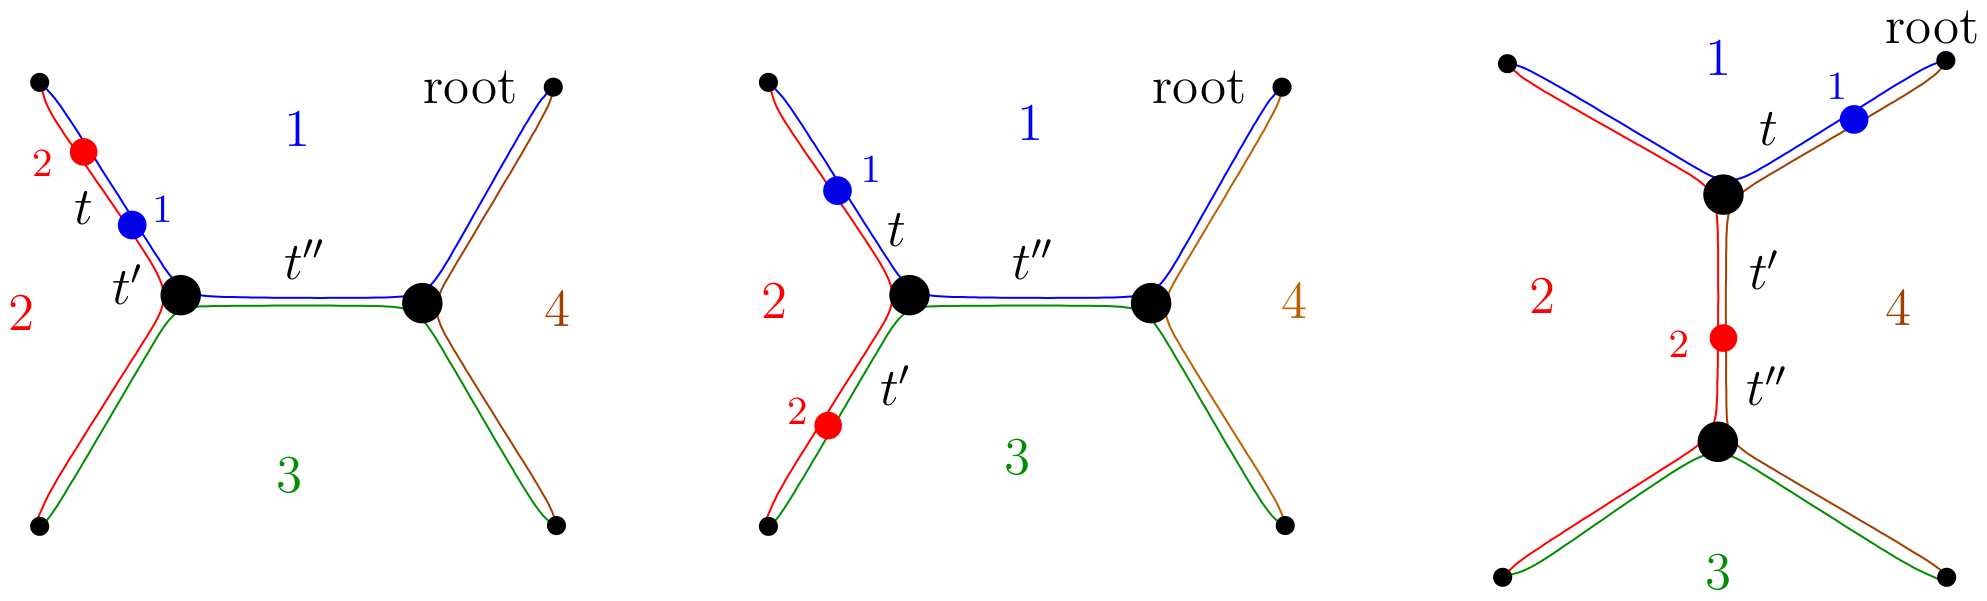
\includegraphics[width=\linewidth]{fig11.png}
  \caption{$MT_{1,2,3,4;1,1,0,0}$ 的三个最高维胞腔。（原书 p.22）}
  \label{fig:11}
\end{figure}

上述构造给出树模空间上的一个微分形式（在 \cite{losev} 的术语中称为前振幅，pre-amplitude）：
\begin{equation}\tag{49}\label{eq:49}
\begin{aligned}
I\in{}&\Omega^\bullet(MT_{a_1,\dots,a_r;k_1,\dots,k_r})\otimes\\
&\otimes\mathrm{Hom}\bigl(\Mor^{\otimes k_1}_{a_1,a_1}\otimes\Mor_{a_1,a_2}\otimes\cdots\otimes\Mor_{a_{r-1},a_r}\otimes\Mor^{\otimes k_r}_{a_r,a_r},\ \Mor_{a_1,a_r}\bigr).
\end{aligned}
\end{equation}
这里我们简记 $\Mor_{a,b}:=\mathbb R\otimes\Mor(F_a,F_b)$，即 $\mathbb{F}$ 中的态射空间与 $\mathbb R$ 的张量积。

% [Tutor Note: 原文 (49) 在两行的行末与行首各印了一个 $\otimes$，照排后出现两个张量积符号，这是排版残留，译文照印未改。另注意输入顺序与式 (3) 一致：先 $\Mor_{a_1,a_1}^{\otimes k_1}$、再 $\Mor_{a_1,a_2}$，例 6 的排法即由此而定；次序写反则 $\int_{MT}I=m$ 不成立。]

\begin{thmenv}{例}{6}\label{ex:6}
例如，对图~\ref{fig:11} 中间那棵树，有
\[
  I(t,\mathrm{d}t,t',\mathrm{d}t',t'',\mathrm{d}t'')(Z_1,[P_{12}],Z_2,[P_{23}],[P_{34}])=\sum_{P_{14}\in\mathrm{Crit}(F_1-F_4)}\bar I\cdot[P_{14}],
\]
其中
\begin{equation}\tag{50}\label{eq:50}
\begin{aligned}
\bar I(t,\mathrm{d}t,t',\mathrm{d}t',t'',\mathrm{d}t'')&=\int_X\delta_{\mathrm{Stab}P_{14}}\wedge\\
&\quad\wedge U_{F_1-F_3}(t'',\mathrm{d}t'')\Bigl(U_{F_1-F_2}(t,\mathrm{d}t)(\delta_{Z_1}\wedge\delta_{\mathrm{Unstab}P_{12}})\\
&\qquad\wedge U_{F_2-F_3}(t',\mathrm{d}t')(\delta_{Z_2}\wedge\delta_{\mathrm{Unstab}P_{23}})\Bigr)\\
&\quad\wedge\delta_{\mathrm{Unstab}P_{34}}.
\end{aligned}
\end{equation}
\end{thmenv}

这里 $\int_X\delta_{\mathrm{Stab}P_{14}}\wedge\cdots$ 是根（“出态”）的贡献。记号 $U_{F_a-F_b}$ 指 $F_a-F_b$ 的梯度向量场所对应的超传播子~\eqref{eq:48}。\footnote{注意，(50) 是式~\eqref{eq:29} 中 $\int_{\mathbb R_+^E}$ 的被积式——取对应图~\ref{fig:11} 中间那棵组合树的项——，其中对 $X^{V\setminus\{q\}}$ 的积分已经算掉；这里 $q$ 是由一条边与根相连的顶点（本例中为右侧的 3 价顶点）。}

% [Tutor Note: (50) 的次数核对法：$U=e^{-tH}(1-\mathrm{d}t\,G)$ 中 $\mathrm{d}t$ 与 $G=\iota_v$ 成对出现，每对净次数为 0，但使 $X$ 方向的形式次数降 1。要对 $X$ 与 $MT$ 同时取顶次项，需三条内部边各取一个 $\mathrm{d}t$（凑出 $\mathrm{d}t\wedge\mathrm{d}t'\wedge\mathrm{d}t''$），且 $\delta_{\mathrm{Stab}P}$、$\delta_{\mathrm{Unstab}P}$、$\delta_Z$ 的次数之和（分别为 $P$ 的指标、$P$ 的余指标、链的余维数）等于 $\dim X+3$。]

\begin{thmenv}{注}{4.1}\label{rem:4.1}
为解析上的方便——若希望入态是相应“态的态空间”中的元素（而不是极限点）——不妨把 delta 形式 $\delta_{\mathrm{Unstab}P}$ 换成它的 $\epsilon$ 光滑化版本 $\delta^{\epsilon}_{\mathrm{Unstab}P}$（同时在 2 价顶点处把正规化 $\delta_Z$ 换成 $\delta^{\epsilon}_Z$），最后在 $I$ 的表达式中取极限 $\epsilon\to0$。
\end{thmenv}

% [Tutor Note: 原文此处印作 “the respective states of states”，疑为 spaces of states 之笔误。译文照印并加引号，读者按“态空间”理解即可。之所以要光滑化：$\delta_{\mathrm{Unstab}P}$ 是分布形式，两个分布形式相乘没有定义，换成 $\delta^\epsilon$ 后所有运算都在光滑形式内完成，最后再取 $\epsilon\to0$。]

形式 $I$ 有三条关键性质。

\begin{enumerate}
  \item[(i)] \textbf{闭性.}\quad 有
  \begin{equation}\tag{51}\label{eq:51}
    (\mathrm{d}_{MT}+Q)I=0,
  \end{equation}
  其中 $\mathrm{d}_{MT}$ 是树模空间上的 de Rham 微分，$Q$ 按导子作用：它在式~\eqref{eq:49} 的每个态射空间上取相应的微分——在 $\Mor(F_a,F_b)$（$a\neq b$）上取 Morse 微分 $\mathrm{d}_{\mathrm{Morse}}$，在奇异链 $\Mor(F_a,F_a)$ 上取边界算子。式~\eqref{eq:51} 成立的原因是：用来构造 $I$ 的超传播子 $U(t,\mathrm{d}t)$ 是 $(\mathrm{d}_t+Q)$-闭的，见式~\eqref{eq:14}。

  % [Tutor Note: 这里的 $Q$ 要读成作用在算符上的分次交换子 $[\mathrm{d}_X,\cdot]$：在微分形式上它就是外微分 $\mathrm{d}$（即第 4.1 节开头的 $Q=\mathrm{d}$），在算符上则是 $[Q,\cdot]$。式 (14) 的 $(\mathrm{d}_t+[\mathrm{d}_X,-])U=0$ 与 (51) 是同一件事。]

  \item[(ii)] \textbf{在红外边界上的分解.}\quad 若图中某条边的长度变为 $+\infty$，则 $I$ 分解。模空间 $MT$ 的红外边界形如 $\bigcup_{i<j}\partial^{IR}_{ij}MT$，其中
  \begin{equation}\tag{52}\label{eq:52}
  \begin{aligned}
  \partial^{IR}_{ij}MT_{a_1,\dots,a_r;k_1,\dots,k_r}\simeq\bigcup_{\substack{k'_i+k''_i=k_i,\\ k'_j+k''_j=k_j}}&MT_{a_1,\dots,a_j;k'_i,k_{i+1},\dots,k_{j-1},k'_j}\\
  &\times MT_{a_1,\dots,a_i,a_j,\dots,a_r;k_1,\dots,k_{i-1},k''_i,k''_j,k_{j+1},\dots,k_r}.
  \end{aligned}
  \end{equation}
  该边界层片对应于把树在 $(a_i,a_j)$-边处剪开（等价于令这条边的长度为 $t=+\infty$）；并取遍把颜色 $a_i$、$a_j$ 的 2 价顶点分配到剪口两侧的所有方式。于是 $I$ 的分解性质指
  \begin{equation}\tag{53}\label{eq:53}
  \begin{aligned}
  I_{a_1,\dots,a_r;k_1,\dots,k_r}\big|_{\partial^{IR}_{ij}}=\sum_{\substack{k'_a+k''_a=k_a,\\ k'_b+k''_b=k_b}}\big\langle&\pi_1^*\bigl(I_{a_1,\dots,a_j;k'_i,k_{i+1},\dots,k_{j-1},k'_j}\bigr),\\
  &\pi_2^*\bigl(I_{a_1,\dots,a_i,a_j,\dots,a_r;k_1,\dots,k_{i-1},k''_i,k''_j,k_{j+1},\dots,k_r}\bigr)\big\rangle,
  \end{aligned}
  \end{equation}
  其中 $\pi_{1,2}$ 是式~\eqref{eq:52} 右端两个因子的投影，$\langle,\rangle$ 是 $MT$ 上微分形式的外积，同时把 $\pi_1^*(I)$ 在 $\Mor_{ab}$ 中的输出代入 $\pi_2^*(I)$ 作为输入；$I$ 的下标标出 $I$ 被限制到 $MT$ 的哪个分支上。分解性质~\eqref{eq:53} 可由式~\eqref{eq:15} 立即推出。

  % [Tutor Note: 式 (52) 的求和条件用位置指标 $i,j$（$k'_i+k''_i=k_i$），式 (53) 却改用 $a,b$（$k'_a+k''_a=k_a$）；按上下文二者指同一对指标，原文如此，译文照印。另注意 (52) 第一因子的颜色列表 $a_1,\dots,a_j$ 有 $j$ 项，而 $k$-序列 $k'_i,k_{i+1},\dots,k_{j-1},k'_j$ 只有 $j-i+1$ 项，项数不符；按剪开 $(a_i,a_j)$-边的几何，第一因子应接 $a_i,\dots,a_j$。原文如此，译文照印，未擅改。]
  % [Tutor Note: 式 (53) 的“立即推出”指：把式 (15) 的 $U(+\infty)=i\circ p$ 作用到那条趋于无穷的边上，$I$ 就裂成两个因子，而 $i\circ p$ 正好把一侧的输出与另一侧的输入对接。对每条趋于无穷的边归纳一次即得 (53)，作者省去了这个逐边归纳。]

  \item[(iii)] \textbf{周期.}\quad
  \begin{equation}\tag{54}\label{eq:54}
    \int_{MT}I=m.
  \end{equation}
  $I$ 在模空间 $MT_{a_1,\dots,a_r;k_1,\dots,k_r}$ 上的积分，就是式~\eqref{eq:3}、\eqref{eq:4} 所定义的复合映射 $m$。这可由构造直接得到，特别地用到式~\eqref{eq:12}。
\end{enumerate}

现在给出 $A_\infty$ 关系式的论证。把式~\eqref{eq:51} 在模空间上积分，并利用 $MT$ 上的 Stokes 定理，得到
\begin{equation}\tag{55}\label{eq:55}
  \int_{\partial MT}I=\pm Q\int_{MT}I.
\end{equation}
右端是 $\pm Qm$，它给出式~\eqref{eq:7} 中内层 $m$ 只作用于单个输入的那些项（即 $s=1$ 的项）。式~\eqref{eq:55} 的左端则是 $I$ 在 $MT$ 的下列各类边界层片上积分之和。

% [Tutor Note: 式 (55) 的 $\pm$ 只来自边界定向的约定：由 (51) 得 $\mathrm{d}_{MT}I=-QI$，两边在 $MT$ 上积分并用 Stokes 定理，左端化为 $\int_{\partial MT}I$，右端为 $-Q\int_{MT}I$（$Q$ 作用在 $X$ 一侧，与 $MT$ 上的积分可交换）。边界取外法向或内法向定向，差别恰是整体符号，故原文写 $\pm$。]

\begin{enumerate}
  \item[(a)] UV 层片：连接两个 3 价顶点的边的长度趋于零。对图的各组合型求和时，这些层片的贡献相互抵消（一个 4 价顶点的两种分解／去收缩的贡献相消）。
  \item[(b)] UV 层片：两个颜色不同（$a$、$b$）的 2 价顶点相撞。两种相撞方向给出的贡献相互抵消。
  \item[(c)] UV 层片：一个 2 价顶点与一个 3 价顶点相撞。2 价顶点沿带的侧边移动时可以从两个方向接近 3 价顶点，这两个方向的贡献相互抵消。
  \item[(d)] UV 层片：两个同色的 2 价顶点相撞。这些贡献不抵消，而是进入式~\eqref{eq:55} 的左端，给出 $A_\infty$ 关系式~\eqref{eq:7} 中形如 $m(\dots,m(Z,Z'),\dots)$ 的项，其中 $Z$、$Z'$ 是两条链。
  \item[(e)] IR 层片：某条内部边的长度变为无穷。由式~\eqref{eq:53} 与~\eqref{eq:54}，在这些情形下式~\eqref{eq:55} 的左端给出 $A_\infty$ 关系式中内层 $m$ 涉及两种或更多颜色的全部项。
\end{enumerate}

总之，式~\eqref{eq:55} 恰好给出范畴 $\mathbb{F}$ 中的 $A_\infty$ 关系式。

\begin{thmenv}{例}{7}\label{ex:7}
考虑颜色为 $a_1=1$、$a_2=2$，且 $k_1=2$、$k_2=1$ 的度量树模空间。把 $(\mathrm{d}_{MT}+Q)I$ 在它上面积分，就得到 $A_\infty$ 关系式（差一个符号）：
\begin{equation}\tag{56}\label{eq:56}
\begin{aligned}
0&=\Bigl(Qm+\int_{\partial MT_{1,2;2,1}}I\Bigr)(Z_1,Z'_1,[P],Z_2)\\
&=\Bigl(\mathrm{d}_{\mathrm{Morse}}m(Z_1,Z'_1,[P],Z_2)+m(\partial Z_1,Z'_1,[P],Z_2)+m(Z_1,\partial Z'_1,[P],Z_2)\\
&\qquad+m(Z_1,Z'_1,\mathrm{d}_{\mathrm{Morse}}[P],Z_2)+m(Z_1,Z'_1,[P],\partial Z_2)\Bigr)\\
&\quad+\Bigl(m(Z_1\cap Z'_1,[P],Z_2)+m(Z_1,m(Z'_1,[P]),Z_2)+m(Z_1,Z'_1,m([P],Z_2))\\
&\qquad+m(m(Z_1,Z'_1,[P]),Z_2)+m(Z_1,m(Z'_1,[P],Z_2))\Bigr).
\end{aligned}
\end{equation}
\end{thmenv}

其中 $Z_1,Z'_1\in\Mor(F_1,F_1)$ 是链，$[P]\in\Mor(F_1,F_2)$ 是 $F_1-F_2$ 的临界点，$Z_2\in\Mor(F_2,F_2)$ 是另一条链。下面用图说明 $\int_{\partial MT}I$ 中各项的来源。

% [Tutor Note: 式 (56) 里 $m$ 有三种用法，极易混：$r=2$ 的 (4)（如 $m(Z_1,Z'_1,[P])$）、$r=1$ 的 (5)（如 $Z_1\cap Z'_1$ 与 $\partial Z_1$）、以及外层 $m$ 吞掉一个内层 $m$ 的嵌套（如 $m(m(Z_1,Z'_1,[P]),Z_2)$）。核对时先按输入的颜色序列判断该用 (4) 还是 (5)。]

\begin{figure}[htbp]
  \centering
  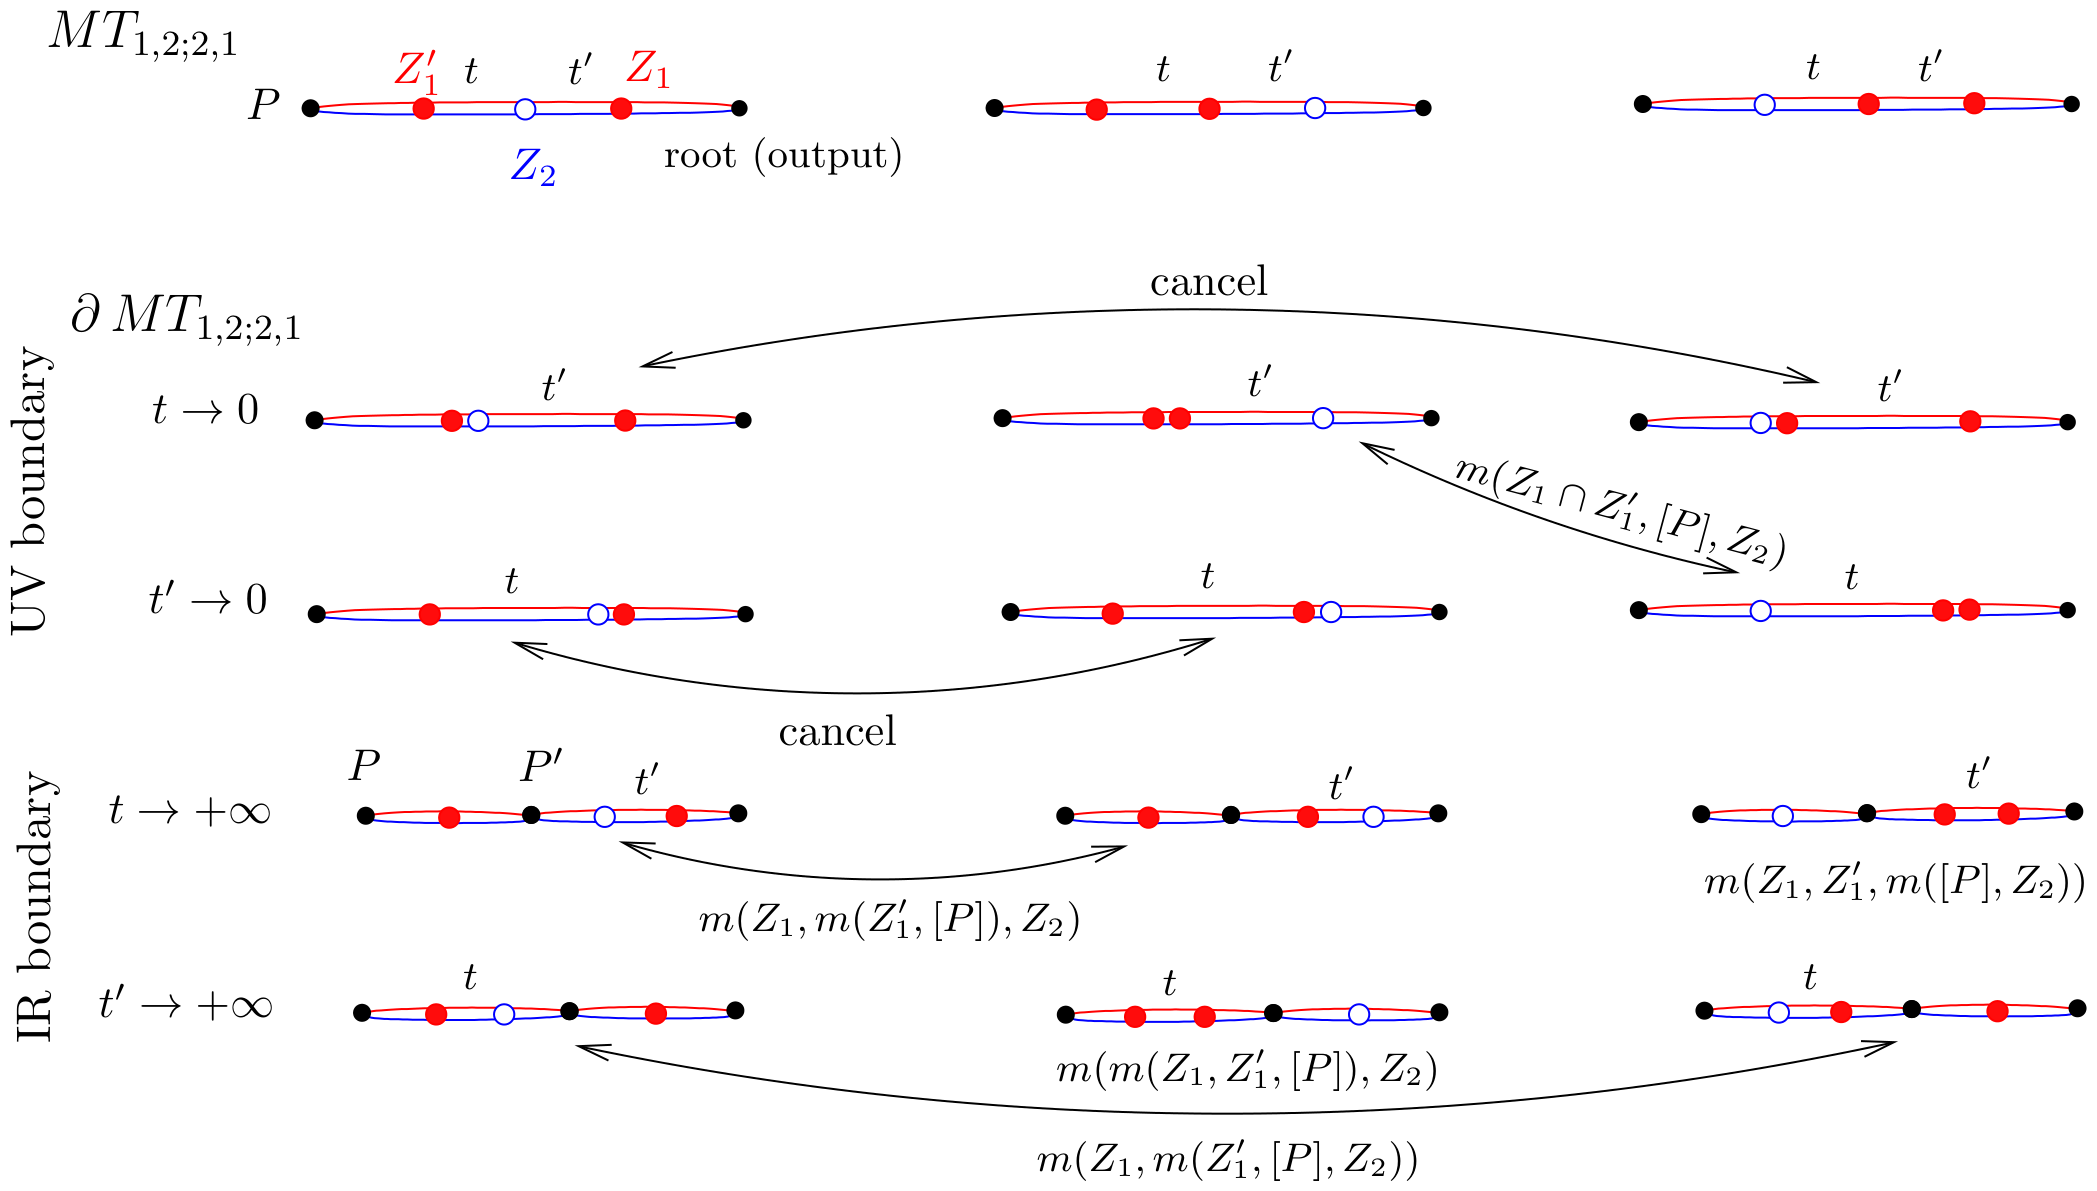
\includegraphics[width=0.98\linewidth]{fig12.png}
  \caption{度量树模空间的边界层片对 $\int_{\partial MT}I$（从而对 $A_\infty$ 关系式）的贡献。（原书 p.25）}
  \label{fig:12}
\end{figure}

\endinput

% =====================================================================
%  第 5 节  结语（原书 p.25）
% =====================================================================
\section{结语}\label{sec:5}

\begin{takeaway}
\begin{itemize}
  \item \textbf{物理图像}：第~\ref{sec:2.4} 节把余维一闭链纳入态射，相当于给对象加上一个平坦联络（局部系统）；把对象换成 $\nu_a$ 个副本（$T^*X$ 语言中的“堆叠”），就得到系数在 $GL(\nu_a)$ 中的非阿贝尔平坦联络。
  \item \textbf{数学工具}：Fukaya 范畴的“堆叠”语言、分块矩阵代数、Morse--Bott 函数与 Morse--Bott 链。
  \item \textbf{主要结论}：全文两个证明都没有用到全纯圆盘这一概念；构造还可推广到 $F_a-F_b$ 仅为 Morse--Bott 的情形，此时 $\Mor(F_a,F_b)$ 取为 $\mathrm{Crit}(F_a-F_b)$ 上的 Morse--Bott 链。
\end{itemize}
\end{takeaway}

按第~\ref{sec:2.4} 节的方式把余维一的闭链纳入进来，可以解释为给一个对象加上平坦联络（局部系统）。其实还可以考虑把对象 $F_a$ 换成 $F_a$ 的 $\nu_a$ 个副本——用 $T^*X$ 的 Fukaya 范畴的语言说，就是 $\nu_a$ 个 Lagrange 子流形 $L_a$ 的“堆叠”。用第~\ref{sec:3} 节的语言，这相当于把 $N\times N$ 矩阵构成的系数代数，换成以 $\nu_a\times\nu_b$ 为块大小的分块矩阵代数。特别地，由此可以对一个对象 $F_a$ 配上 $X$ 上（或用 $T^*X$ 的语言，$L_a$ 上）系数在 $GL(\nu_a)$ 中的非阿贝尔平坦联络。

% [Tutor Note: 余维一闭链与平坦联络的对应来自式 (5)：$m(Z_1,Z_2)=Z_1\cap Z_2$ 是链的带符号相交。取 $Z$ 为余维一闭链时，相交数给出绕该闭链一周的相位，这正是和乐；把系数换成 $GL(\nu_a)$ 矩阵，和乐就成为非阿贝尔的。作者没有展开这个对应，正文只用了「可以解释为」的说法。]

% [Tutor Note: “堆叠”是 $T^*X$ 的 Fukaya 范畴中的标准图像：一个 Lagrange 子流形取 $\nu$ 个重合副本，其上的规范场联络自然取 $GL(\nu)$ 值。注意这里的副本不是“扰动开来的”，而是重合的；若真的扰动开，全纯圆盘会重新出现，反而不属于本文的框架。]

注意，无论是在 $A_\infty$ 关系式的第一个证明（用有效作用量）中，还是在第二个证明（用拓扑量子力学）中，我们都没有用到全纯圆盘这一概念。

我们还要指出，本文的构造可以推广到如下情形：函数差 $F_a-F_b$ 只要求是 Morse--Bott 的，而不必是 Morse 的。此时临界集 $\mathrm{Crit}(F_a-F_b)$ 允许是不同维数的子流形之并，而不限于孤立点集。于是把 $\Mor(F_a,F_b)$ 取为 $\mathrm{Crit}(F_a-F_b)$ 上的奇异链，并配以 Morse--Bott 微分；该微分把链上的边界算子与临界流形之间梯度流的数据结合起来。注意，在这一处理方式下，无需单独讨论对象 $F_a$ 到自身的态射——它是上述一般构造的一个特例（事实上 $\mathrm{Crit}(F_a-F_a)=X$，因此此时的 Morse--Bott 链就是 $X$ 上的奇异链）。

% [Tutor Note: 末句把 §2.1 的“特设”模型解释成一般构造的推论：$F_a-F_a\equiv0$ 的临界集是整个 $X$，故自同态的 Morse--Bott 链复形就是 $X$ 上的奇异链，与式 (2) 一致。但要注意 Morse--Bott 微分比链的边界算子多一项——临界流形之间的梯度流；在 $a=b$ 的特例里这一项退化，所以 (2) 只需边界算子。]

\endinput


% =====================================================================
%  参考文献（原书 p.26–27）—— 条目序即原文编号 [1]–[17]，保持英文原样
%  引用请用 \cite{键}，键表见 work/citations.md
% =====================================================================
\section*{参考文献}
\addcontentsline{toc}{section}{参考文献}

\begingroup
\small
\begin{thebibliography}{17}

\bibitem{auroux}
D.~Auroux, ``A beginner's introduction to Fukaya categories,'' in \emph{Contact and symplectic topology}, pp.~85--136. Springer, Cham, 2014.

\bibitem{cattaneo}
A.~S.~Cattaneo, C.~A.~Rossi, ``Higher-Dimensional BF Theories in the Batalin--Vilkovisky Formalism: The BV Action and Generalized Wilson Loops,'' \emph{Commun. Math. Phys.} \textbf{221}.3 (2001) 591--657.

\bibitem{crainic}
M.~Crainic, ``On the perturbation lemma, and deformations,'' arXiv preprint math/0403266.

\bibitem{frenkel}
E.~Frenkel, A.~Losev, N.~Nekrasov, ``Instantons beyond topological theory. I.'' \emph{Journal of the Institute of Mathematics of Jussieu} \textbf{10}, no.~3 (2011): 463--565.

\bibitem{fukaya}
K.~Fukaya, ``Morse homotopy, $A_\infty$-category and Floer homologies.'' In \emph{Proceeding of Garc Workshop on Geometry and Topology}. Seoul National Univ, 1993.

\bibitem{fukayaoh}
K.~Fukaya, Y.~G.~Oh, ``Zero-loop open strings in the cotangent bundle and Morse homotopy,'' \emph{Asian Journal of Mathematics} \textbf{1}, no.~1 (1997): 96--180.

\bibitem{fukayaetal}
K.~Fukaya, Y.~G.~Oh, H.~Ohta, K.~Ono, ``Lagrangian intersection Floer theory: anomaly and obstruction, I and II,'' AMS 2009.

\bibitem{gugenheim}
V.~K.~A.~M.~Gugenheim, ``On the chain-complex of a fibration,'' \emph{Illinois Journal of Mathematics} \textbf{16} (1972) 398--414.

\bibitem{lambe}
L.~Lambe, J.~Stasheff, ``Applications of Perturbation Theory to iterated fibrations,'' \emph{Manuscripta Mathematica} \textbf{58} (1987) 363--376.

\bibitem{losev}
A.~Losev, ``TQFT, homological algebra and elements of K.~Saito's theory of Primitive form: an attempt of mathematical text written by mathematical physicist.'' In \emph{Primitive Forms and Related Subjects---Kavli IPMU 2014}, pp.~269--293. Mathematical Society of Japan, 2019.

\bibitem{losevpolyubin}
A.~Losev, I.~Polyubin, ``Topological quantum mechanics for physicists.'' \emph{Journal of Experimental and Theoretical Physics Letters} \textbf{82}, no.~6 (2005): 335--342.

\bibitem{lysov}
V.~Lysov, ``Anticommutativity equation in topological quantum mechanics.'' \emph{Journal of Experimental and Theoretical Physics Letters} \textbf{76}, no.~12 (2002): 724--727.

\bibitem{kontsevichmanin}
M.~Kontsevich, Yu.~Manin, ``Gromov-Witten classes, quantum cohomology, and enumerative geometry.'' \emph{Communications in Mathematical Physics} \textbf{164}, no.~3 (1994): 525--562.

\bibitem{kontsevichsoibelman}
M.~Kontsevich, Y.~Soibelman, ``Homological mirror symmetry and torus fibrations.'' arXiv preprint math/0011041 (2000).

\bibitem{mnev}
P.~Mnev, ``Discrete BF theory,'' arXiv:0809.1160.

\bibitem{seidel}
P.~Seidel, \emph{Fukaya Categories and Picard-Lefschetz Theory}, Zurich Lectures in Advanced Mathematics. European Mathematical Society (EMS), Zurich, 2008.

\bibitem{witten}
E.~Witten, ``Supersymmetry and Morse theory,'' \emph{Journal of Differential Geometry} \textbf{17}, no.~4 (1982): 661--692.

\end{thebibliography}
\endgroup

\bigskip
\noindent\rule{\linewidth}{0.4pt}
\noindent\textbf{作者单位（照录原文）}

\smallskip
\noindent{\footnotesize
University of Connecticut, Department of Mathematics, Storrs, CT 06269, USA\\
Email address: \texttt{[邮箱隐去]}

\smallskip
Wu Wen-Tsun Key Lab of Mathematics, Chinese Academy of Sciences, USTC,\\
No.96, JinZhai Road Baohe District, Hefei, Anhui, 230026, P.R.China\\
National Research University Higher School of Economics, Laboratory of Mirror Symmetry, NRU HSE, 6 Usacheva str., Moscow, Russia, 119048\\
Federal Science Centre ``Science Research Institute of System Analysis at Russian Science Academy'' (GNU FNC NIISI RAN), Nakhimovskiy pr. 36-1, Moscow, Russia, 117218\\
Email address: \texttt{[邮箱隐去]}

\smallskip
University of Notre Dame, Notre Dame, IN 46556, USA\\
St. Petersburg Department of V.~A.~Steklov Institute of Mathematics of the Russian Academy of Sciences, 27 Fontanka, St. Petersburg, Russia, 191023\\
Email address: \texttt{[邮箱隐去]}

\smallskip
Albert Einstein Center for Fundamental Physics, Institute for Theoretical Physics, University of Bern, Hochschulstrasse 6, 3012 Bern, Switzerland\\
Email address: \texttt{[邮箱隐去]}
}
\endinput


% =====================================================================
%  附录（批注一览；由 work/gen_notes.py 从各章源码自动生成，勿手改）
% =====================================================================
\appendix
\ifshownotes
  % 由 work/gen_notes.py 自动生成，请勿手改。
\section{译校批注一览}\label{app:notes}

\noindent 全文共 \textbf{68} 条译校批注。每条的原始位置在对应段落之后的 LaTeX 注释里（\verb|% [Tutor Note: …]|），不进入排版结果；本附录按节次汇总，便于对照原文复查。

\subsection*{第 1 节 引言}
\begin{enumerate}
  \item 本节是全文的路标，一句话概括：把 Fukaya 范畴在余切丛 $T^*X$ 上取半经典极限 $\epsilon\to0$，全纯圆盘的计数就退化为梯度流树的计数；本文补上“对象到自身”的态射，并给出 $A_\infty$ 关系式的两个非全纯证明。\hfill{\footnotesize （源码第 6 行）}
  \item “重标度 $F_a\to\epsilon F_a$”是全篇第一个易错点：$\epsilon\to0$ 时 $L_a=\mathrm{graph}(\epsilon\,\mathrm{d}F_a)$ 退化到零截面，交点 $P_{\alpha,ab}$ 趋于 $\mathrm{d}(F_a-F_b)=0$ 的临界点，全纯圆盘的半径随之趋于零。作者在此省略了“一列全纯圆盘收敛到梯度流树”的紧性论证，标准做法是用 Gromov 紧性与 $T^*X$ 上近全纯曲线的局部描述，见 Fukaya--Oh \cite{fukayaoh} 与 Seidel \cite{seidel} 第 9 章。\hfill{\footnotesize （源码第 26 行）}
  \item “两个证明都不涉及全纯圆盘”是全文纲领，值得停一下。其一只用 BV 形式的纤维积分与树形求和（等价于 Kontsevich--Soibelman 同伦转移定理，见 \cite{kontsevichsoibelman}）；其二只用度量树模空间上一个闭微分形式与 Stokes 定理。换言之，作者把“辛几何”这一层完全剥离，只留下“生成函数之差是 Morse--Smale 函数”与“梯度流”两件事。这也解释了为什么证明能同时给出整系数版本与一般的环系数版本。\hfill{\footnotesize （源码第 30 行）}
  \item (B) 的逻辑方向容易说反。BV 主方程 $\{S_{\mathrm{eff}},S_{\mathrm{eff}}\}=0$ 直接给出的是 $L_\infty$ 关系式（斜对称化之后的结果）；要得到 $A_\infty$ 关系式，必须把系数代数换成上三角矩阵代数 $\mathcal A$ 再张量，见注 3.2 与式 (47)。作者在 (B) 里没有点破这一层，读者若不留意会误以为 $A_\infty$ 关系式可以直接从 BV 主方程读出。\hfill{\footnotesize （源码第 54 行）}
  \item (A) 中“取奇异链”不是任意选择：$F_a-F_a\equiv0$ 的临界点集是整个 $X$，故自同态的 Morse 复数形式上就是 $X$ 上的链；取奇异链（而非只取点）使复合映射 (4) 能作用在“被看作分布”的链上。若改取 de Rham 形式或上链，会付出别的代价，见第 2.7 节与我在此处的批注。\hfill{\footnotesize （源码第 56 行）}
\end{enumerate}

\subsection*{第 2 节、第 2.1 节}
\begin{enumerate}
  \item 读本节前先记住一个总原则：这个范畴里所有“数出来的整数”都带符号，符号由 Morse 理论的有向计数给出；而所有横截性问题都靠“假设 2.2”回避，而不是靠扰动具体实现。作者把这一取舍称为“部分定义”，这是理解后文两个证明为何都用“无穷小邻域/光滑化”操作的前提。\hfill{\footnotesize （源码第 18 行）}
  \item 式 (1) 的下标约定极易出错：$P_{ab}$ 中前一个下标 $a$ 是源（$F_a$），后一个 $b$ 是靶（$F_b$），与函数差写成 $F_a-F_b$ 的顺序一致。若误按 $F_b-F_a$ 理解，Morse 指标会整体反号，式 (4) 的树形规则也随之颠倒。核对原书 p.4 式 (4) 与其后的三价顶点规则。\hfill{\footnotesize （源码第 40 行）}
  \item 提示“按余维数分级”与“按余指标分级”是同一件事的两种说法，但只差一个整体次数平移：$\operatorname{codim}=\dim X-\operatorname{coind}$。作者在 (1)(2) 中并列使用两种分级，正是为了让式 (3) 的次数公式 $2-n$ 在两块上都成立；这一处若统一成“按维数分级”，所有公式都要整体加 $\dim X$ 的平移，切勿随手统一。\hfill{\footnotesize （源码第 42 行）}
  \item 式 (4) 中 $\#\mathcal M$ 的参数写作 $P_{12}$，而式 (4) 左侧与求和处写作 $P_{a_1a_2}$。这是原文的记号不一致（疑为缩写或笔误），译文照录不改；读者把它读作 $P_{a_1a_2}$ 即可。\hfill{\footnotesize （源码第 88 行）}
  \item 三价顶点的颜色规则 $(a,b),(b,c)\to(a,c)$ 是说：沿树从叶到根走，标号必须“接力”，且每经过一个三价顶点就换一次色。这条规则把树的组合型与复合的输入顺序绑在一起，是全节最实质的约定；它同时也是“不需要四价顶点”的原因——四价顶点的两种分解在同调层面相消（见第 4.2 节 (a) 类边界层片的讨论）。\hfill{\footnotesize （源码第 90 行）}
  \item 这里“反推”用的是循环形式的配对 $\langle x_0,m(x_1,\dots,x_p)\rangle$，而不是 (4) 的非循环版本；两者相差一个取对偶的手续，符号来自 $\dim X$ 次的交换（见前一条批注）。若直接对 (4) 取 $a_1=a_r$，会多出一个不属于树的边界项，这是最容易算错的一步。\hfill{\footnotesize （源码第 106 行）}
  \item 式 (7) 中的 $\pm$ 号在原文里没有显式写出，它是 Koszul 符号：当内层 $m$ 的次数为奇时要对换序引入符号，具体为 $(-1)^{|x_1|+\cdots+|x_r|}$ 型的因子。这是全节唯一“不显式”的地方，定理 1 的两个证明（第 3、4 节）都给出同一符号约定；若读者自行补证，务必先固定 Koszul 约定，否则会差出整体符号。\hfill{\footnotesize （源码第 118 行）}
  \item 定理 1 的证明不是本节给出，而是第 3、4 节的两个独立证明。这是本文的组织方式：先把范畴定义“数”出来，再用两种场论把关系式“证”出来。阅读时建议先接受定理 1，直接进入第 3 节看有效作用量如何把它变成一个 BV 主方程。\hfill{\footnotesize （源码第 120 行）}
\end{enumerate}

\subsection*{第 2.2–2.3 节}
\begin{enumerate}
  \item 图 1 中边上的数字 1、2、3 是三个对象的标号（对应图 2 的 $L_1,L_2,L_3$ 即圆盘的三段边界弧），不是边的编号。每条边另带双指标 $(a,b)$ 与方向：$P_{12}$、$P_{23}$ 是叶，$P_{13}$ 是根，方向由叶指向根；方向读反，复合的输入与输出就对调。\hfill{\footnotesize （源码第 30 行）}
  \item 图 2 中间那幅画在 $T^*X$ 里：$L_a=\mathrm{graph}(\epsilon\,\mathrm{d}F_a)$ 是恰当 Lagrange 子流形，投影 $T^*X\to X$ 把它压到 $X$ 上。$\epsilon\to0$ 时全纯圆盘的面积趋于零，圆盘的极限是梯度流树；这里的“全纯”一律指伪全纯（见第 1 节脚注 1）。紧性论证原文未写，可参看 \cite{fukayaoh}。\hfill{\footnotesize （源码第 41 行）}
  \item 维数公式逐项对账：$\operatorname{ind}$ 是 $F_1-F_2$ 的 Morse 指标；$P\to P'$ 的轨道模空间维数为 $\operatorname{ind}(P)-\operatorname{ind}(P')$，再减 1 是去掉梯度流的 $\mathbb R$-平移。每个 2 价顶点是一条边与链 $Z$ 的交点：链的余维数为 $c$ 时只贡献 $c-1$ 个条件，因为交点沿 1 维的边可自动滑动。另注意 (1) 按余指标分级，此处用指标，二者只差常数 $\dim X$，差值不变。\hfill{\footnotesize （源码第 79 行）}
  \item 把 (7) 按 $n=2$ 展开：$r=0,s=1$ 给出 $m(\mathrm{d}x_1,x_2)$，$r=1,s=1$ 给出 $m(x_1,\mathrm{d}x_2)$，$r=0,s=2$ 给出 $\mathrm{d}m(x_1,x_2)$，正是 (8) 的三项。注意 $x_2=Z$ 是链，其微分是边界算子，故第二项写作 $m([P],\partial Z)$ 而非 $m([P],\mathrm{d}Z)$；$x_1=[P]$ 是 Morse 链，$\mathrm{d}_{\mathrm{Morse}}[P]=[R]$ 即式 (8) 中的下花括号。\hfill{\footnotesize （源码第 100 行）}
  \item (9) 中 $\mathcal L_v$ 是李导数，$\iota_v$ 是内乘（interior product）。$U$ 的 0 次部分是拉回 $e^{-t\mathcal L_v}$，1 次部分是 $-\mathrm{d}t\,e^{-t\mathcal L_v}\iota_v$，故 (12) 的负号来自这里；$\int_0^\infty U(t,\mathrm{d}t)$ 只取 $\mathrm{d}t$ 分量，即在 $(0,+\infty)$ 上积一个 1 次形式。把 $\iota_v$ 从 $e^{-t\mathcal L_v}$ 右边挪到左边不变号，因为 $v$ 在自身的流下不变：$e^{-t\mathcal L_v}\iota_v=\iota_v e^{-t\mathcal L_v}$。\hfill{\footnotesize （源码第 120 行）}
  \item $i$ 用不稳定流形、$p$ 用稳定流形，二者不可互换。$p\circ i=\mathrm{id}$ 的道理是：$\delta_{\mathrm{Unstab}_Q}$ 的余维数为 $\operatorname{ind}Q$，沿维数为 $\operatorname{ind}P$ 的 $\mathrm{Stab}_P$ 积分，只有 $\operatorname{ind}P=\operatorname{ind}Q$ 时可能非零；此时 $P\to Q$ 的梯度轨道必为常值，故只有 $P=Q$ 贡献 1。\hfill{\footnotesize （源码第 147 行）}
  \item $U=e^{-(\mathrm{d}_t+[\mathrm{d}_X,-])(t\iota_v)}$ 是简写，不是通常的算子指数：指数里的因子并不交换。用 $[\mathrm{d},\iota_v]=\mathcal L_v$ 可算出 $(\mathrm{d}_t+[\mathrm{d}_X,-])(t\iota_v)=t\mathcal L_v+\mathrm{d}t\,\iota_v$；作者实际取的定义是 (9)，两种写法给出同一个满足 (14) 的形式。\hfill{\footnotesize （源码第 164 行）}
  \item 原文 p.8 此处作 the gradient trajectory of starting at y，多一个 of，疑为笔误；译文按 the gradient trajectory starting at y 理解，其余照录。另注意 $\widetilde Y$ 不是子流形：它是映照 $(t,y)\mapsto(\mathrm{Flow}_t(v)(y),y)$ 在 $(0,+\infty)\times X$ 上的像，边界由 $t=0$ 处的 $\mathrm{Diag}$ 与 $t=+\infty$ 处的 $Y_{+\infty}$ 拼成，这里的 $\partial$ 是链（current）意义下的边界。\hfill{\footnotesize （源码第 172 行）}
  \item (18) 中间的等号关键是 $R_\epsilon$ 与恒等映射链同伦：$R_\epsilon-\mathrm{id}=\mathrm{d}h_\epsilon+h_\epsilon\mathrm{d}$，而 $\delta^\epsilon_{Z_1}$ 闭，被积式又是顶次形式。于是把 $\delta^\epsilon_{Z_2}$ 换回 $\delta_{Z_2}$ 只差一个恰当形式的积分，在闭流形 $X$ 上为零。原文只写“$\epsilon$ 充分小”，这一步省略了。\hfill{\footnotesize （源码第 192 行）}
  \item 正规化的动机：未正规化的 $i$ 取值在分布形式中（含 delta），而 $p$ 只定义在光滑形式上；后文的树形求和要反复做形式乘法，故必须先把对象换成光滑的。$K^\epsilon=R_\epsilon K+h_\epsilon$ 中的 $h_\epsilon$ 不是可选项：它恰好补上 $R_\epsilon$ 与 $\mathrm{id}$ 之间的链同伦缺口，缺了它 (21) 不成立。\hfill{\footnotesize （源码第 224 行）}
\end{enumerate}

\subsection*{第 2.4–2.6 节}
\begin{enumerate}
  \item 此处极易把符号搞反：正确的约定是 $|T_\alpha|=1-\operatorname{codim}C_\alpha$，而不是 $\operatorname{codim}C_\alpha-1$。按前者，例 4 中 $\operatorname{codim}C=1$ 给出 $|T|=0$，故 $e^T$ 的展开不带附加符号；若按后者则 $|T|=-2$，$m(T)$ 的奇偶性与 $e^T-1$ 的符号会整体改变，式 (25) 的符号也随之失配。\hfill{\footnotesize （源码第 27 行）}
  \item 为什么模型中要张量 $\mathbb Q$：Morse 链复形本来定义在 $\mathbb Z$ 上，但重复闭链的位移正规化（注~\ref{rem:2.1}）会产生 $1/k!$ 型的有理系数，$m(T)$ 因而只在张量 $\mathbb Q$ 之后才成为良定义的自同态。若忽略这一点，会误以为 $m(T)$ 保持整系数，进而误判整系数版本是否存在。\hfill{\footnotesize （源码第 35 行）}
  \item 对称化给出的权重是 $T^2/2$，不是笔误：$C$ 的两份副本各得 $1/2$ 的权重，分母上的 $2=2!$；推广到 $k$ 份相互重复的副本时权重为 $1/k!$，这正是例 4 与本节第二个脚注（原书脚注 8）中系数 $1/k!$ 的来源。只有当位移足够小时，对称化的结果才等于 $\tfrac12\sum_\gamma(\#(\gamma\cap C))^2$。\hfill{\footnotesize （源码第 43 行）}
  \item 为什么 $\mathrm{d}_{\mathrm{Morse}}=0$：在圆上，从极大点 $P$ 到极小点 $Q$ 恰有两条梯度轨道（沿两侧各一段半圆），二者定向相反，带符号计数相互抵消。而 $m_P^Q(T)$ 数的是经过闭链副本的轨道：对每组位移，按正确次序经过副本的轨道恰有一条，对称化后得 $1/k!$，累加即 $e^T-1=\sum_{k\ge 1}T^k/k!$。\hfill{\footnotesize （源码第 71 行）}
  \item 作者说“显然”，实际用到两步：其一，$\epsilon\to0$ 时 $\delta^\epsilon_C$ 弱收敛到 $\delta_C$，$K^\epsilon$ 的积分核收敛到 $\delta_{\widetilde Y}$（式 (17) 与第 2.3 节的正则化构造）；其二，沿 $X^V$ 的积分在横截性下化为交点计数。标准出处是 Gugenheim \cite{gugenheim} 与 Lambe--Stasheff \cite{lambe} 的扰动引理，综述见 Crainic \cite{crainic}。\hfill{\footnotesize （源码第 104 行）}
  \item 本段 $m=r-2+\sum_i k_i$ 中的 $m$ 是空间 $X^m$ 的指数（内部顶点总数），与复合映射 $m$ 无关；同段 $Z_{\alpha,a}$ 的下标 $a$ 与临界点 $P_{ab}$ 的双指标也各有含义，读式 (28) 时先分清这两套指标。\hfill{\footnotesize （源码第 132 行）}
  \item $\pi_e^{-1}\widetilde Y_e$ 里的波浪号不能丢：$\widetilde Y_e=\bigcup_{t>0}Y_t$ 是式 (17) 中 $X\times X$ 内的整条扩展轨道族的链，而 $Y_t$ 只是 $t$ 时刻的流动像。$\pi_e$ 把 $X^V$ 投到第 $q_1,q_2$ 份 $X\times X$，$\pi_q$ 只投到单个 $X$，两者的纤维维数不同，把 $\pi_q^{-1}(\widetilde Y_e)$ 写进公式是错的。\hfill{\footnotesize （源码第 143 行）}
  \item 疑似笔误：原书 p.13 把维数公式排成两行，第一行以 $\dim\mathcal M=$ 结尾，第二行又以 $=$ 起头，于是等号出现两次。译文照印，未删去第二个等号；按上下文，第一个等号后应直接接第二行的右端。\hfill{\footnotesize （源码第 161 行）}
  \item “预期维数为零”来自式 (28) 后的维数公式，作者没有写出代入过程：此处 $\operatorname{coind}(\mathbf S)-1=2-1=1$，$-\bigl(\operatorname{coind}(\mathbf N)-1\bigr)=-(0-1)=1$，两条链贡献 $-\bigl((1-1)+(2-1)\bigr)=-1$，最后再减 1，合计 $1+1-1-1=0$。实际模空间是一维的，故横截性必然失效。\hfill{\footnotesize （源码第 182 行）}
  \item 疑似笔误：式 (31) 的乘积写作 $\prod_{a=1}^{N-1}$，但被积函数里是 $\delta_{\mathrm{Unstab}_{P_{a_ia_{i+1}}}}$，下标是 $i$ 而不是 $a$；照式 (29) 应为 $\prod_{i=1}^{r-1}$，或把被积函数的下标改成 $P_{a\,a+1}$。另外这里的 $N-1$ 与式 (29) 的 $r-1$ 也不一致（$N$ 是对象个数，$r$ 是树中叶子个数）。译文照原样排印，未擅改。\hfill{\footnotesize （源码第 233 行）}
  \item 末句的“波前集横截”是关键：Hörmander 的波前集理论断言，两个分布之积有定义当且仅当二者的波前集沿对角逐点横截。$\delta_Z$ 的波前集是 $Z\subset X$ 的余法丛，故对 $X^V$ 上各拉回形式的乘积而言，横截性条件恰是假设~\ref{ass:2.2} 的相交横截性。可参看 Hörmander《The Analysis of Linear Partial Differential Operators》第 8 章。\hfill{\footnotesize （源码第 235 行）}
\end{enumerate}

\subsection*{第 2.7 节、第 3 节}
\begin{enumerate}
  \item 这里三类 $\delta$ 的含义不同：$\delta_{Z_q}$ 是链的 delta 形式（对链积分即数交点），$\delta_{\mathrm{Unstab}_{P_{a_ia_{i+1}}}}$ 与 $\delta_{\mathrm{Stab}_{P_{a_1a_r}}}$ 是稳定、不稳定流形的 delta 形式，而 $\epsilon$-光滑化 delta 形式是链的 delta 形式的正则化。把三类混为一谈，就会误以为链与临界点在这个变体里地位相同。\hfill{\footnotesize （源码第 16 行）}
  \item 为什么 cup 积不需要横截性、而链的相交需要？cup 积是上链层面的代数运算，任意两条上链都可以相乘；链的相交则要求子流形横截，否则交点集不是离散的，计数无意义。但高阶复合仍要数 Morse 树与链的交，所以横截性没有消失，只是从基本运算挪到了复合这一步——这正是作者说「仍得到部分定义的范畴」的原因。\hfill{\footnotesize （源码第 20 行）}
  \item 本节与第 4 节是定理~\ref{thm:1} 的两个独立证明。核心工具是同伦转移的存在性：给定收缩数据 $(i,\mathrm{p},K)$ 后，只要树形求和按次数逐次有限（Morse 收缩经正规化后满足这一条），dg 代数结构就能搬到 $\mathbb{M}$ 上。标准陈述是同调扰动引理，见 \cite{crainic,gugenheim,lambe}；树形求和的具体形状即 Kontsevich--Soibelman 公式 \cite{kontsevichsoibelman}。\hfill{\footnotesize （源码第 32 行）}
  \item 收缩三元组的标准条件是 $\mathrm{p}\,\mathrm{i}=\mathrm{id}_{\mathbb{M}}$ 与 $\mathrm{i}\,\mathrm{p}-\mathrm{id}_V=d_VK+Kd_V$（符号随分级约定略有出入），且 $K$ 的次数为 $-1$。$(a,a)$ 分块取 $\mathrm{i}=\mathrm{p}=\mathrm{id}$、$K=0$，是全篇「增强」的来源：$F_a-F_a\equiv0$ 没有 Morse 理论可用，故 $\Omega_{aa}$ 原样留在 $\mathbb{M}$ 中，不做 Morse 收缩。\hfill{\footnotesize （源码第 66 行）}
  \item 次数核对：$n$ 叶二叉有根树有 $n-1$ 个内部顶点、$n-2$ 条内部边；乘积次数为 $0$，$K$ 的次数为 $-1$，故 $\mu_n$ 的次数为 $2-n$，与式~\eqref{eq:3} 中复合映射的次数一致。若把 $K$ 与乘积的次数记反，式~\eqref{eq:36} 的符号会整体错位。\hfill{\footnotesize （源码第 83 行）}
  \item 上式原书是手绘的二叉树（叶装饰 $\mathrm{i}(X_1),\mathrm{i}(X_2),\mathrm{i}(X_3)$，先由乘积合并前两个叶，在内部边上作用 $K$ 后再与第三个叶相乘，最后在根处作用 $\mathrm{p}$）。译文按原式整行裁图插入（图文件 \mbox{figtree33.png}），未重排；其组合型由「$n$ 叶二叉有根树」与上面的装饰规则唯一决定。\hfill{\footnotesize （源码第 84 行）}
  \item $X_i$ 落在哪个分块极易记错：$a_i\neq a_{i+1}$ 时 $X_i=x_i$ 是 $\mathbb{M}_{a_ia_{i+1}}=\mathrm{MC}(F_{a_i}-F_{a_{i+1}})$ 中的临界点或 Morse 链；$a_i=a_{i+1}$ 时 $X_i=\delta^{\epsilon}_{x_i}$ 落在 $\Omega_{a_ia_i}$ 中。$\delta^{\epsilon}_{x_i}$ 不是临界点，必须当作光滑化 delta 形式才能进入树形公式~\eqref{eq:33}。\hfill{\footnotesize （源码第 96 行）}
  \item 这一步是式~\eqref{eq:33} 与式~\eqref{eq:31} 逐项对应的组合核心。式~\eqref{eq:31} 的树允许 2 价顶点来承载链 $Z_{\alpha,a}$；而式~\eqref{eq:33} 的二叉树叶在 $a_i=a_{i+1}$ 时带的是 $\delta^{\epsilon}_{x_i}$。截去这样的叶及其边，相当于把它并进 $\delta_{Z}$ 型因子，同时在 $T'$ 中留出一个 2 价顶点。图~\ref{fig:8} 给出的正是最简单的例子。\hfill{\footnotesize （源码第 102 行）}
  \item 原书 p.17 把 Soibelman 拼作 Soibleman，疑为笔误；译文照录，未擅改。读者应把它与 \cite{kontsevichsoibelman} 中的 Soibelman 认作同一人，切勿当成另一文献。\hfill{\footnotesize （源码第 118 行）}
  \item 式~\eqref{eq:37} 有三层结构：$A$ 的矩阵指标在 $N\times N$ 上（对应 $\mathbb{F}$ 的 $N$ 个对象），每个矩阵元再取值于 $\mathcal A$（大型上三角矩阵代数）。$\langle\,,\rangle$ 是 $\mathfrak g$ 与 $\mathfrak g^*$ 的配对；对微分形式还要配上 wedge 积与矩阵迹，原文按标准 BF 记号省略未写。$A$ 是奇变量，故 $dA+\frac12[A,A]$ 就是曲率。\hfill{\footnotesize （源码第 136 行）}
  \item 为何必须把系数扩成 $\mathcal A$：只取 $N\times N$ 矩阵时，反对称化后只能读到 $L_\infty$ 括号，$\Ainf$ 的 $\mu_n$ 被混同。张量 $\mathcal A$ 之后，矩阵单位 $t_{ij}$ 像「标签」一样把输入与输出的次序记下来（见式~\eqref{eq:47}）。再取正向极限 $\widetilde N\to\infty$，是为了不设 arity 的上限。$\mathcal A$ 幂零这一点，在「非幂零 $\mathfrak g$」那条脚注处会用到。\hfill{\footnotesize （源码第 142 行）}
  \item 式~\eqref{eq:38} 把「几何」塞进了规范固定：$\iota_{v_{ab}}$ 是沿梯度场 $v_{ab}$ 的缩并。作者断言这个条件等价于「$(A_W)_{ab}$ 被 Morse 链同伦式~\eqref{eq:12} 湮灭」。结合下文 $\mathcal L=\mathrm{im}K\oplus\mathrm{im}K$，这条等价关系正是「几何规范固定转化为内部边装饰 $K$」的翻译词典，也是全节物理思想的关键一步。\hfill{\footnotesize （源码第 150 行）}
  \item 式~\eqref{eq:40} 两端的方括号是次数平移：$[1]$ 与 $[\dim X-2]$ 必须逐项对齐，混淆两者会破坏奇辛配对的次数。右端 $\mathbb{M}\otimes\mathcal A^*$ 中的星号是对 $\mathcal A$ 取对偶，不是对整个张量积取对偶。$\mathcal L=\mathrm{im}K\oplus\mathrm{im}K$ 说明纤维积分沿 $K$ 的像进行，故内部边最终由 $K$ 装饰。\hfill{\footnotesize （源码第 166 行）}
  \item 系数与 $|\mathrm{Aut}(\Gamma)|$ 对应：前三个单链树的权重是 $1/2$；最后的「哑铃」树两条 $K$ 边可交换，自同构群阶为 $8$，故系数是 $1/8$ 而不是 $1/4$。抄写式~\eqref{eq:42} 时最易在此出错，请对原书 p.18 第二行逐字核对。\hfill{\footnotesize （源码第 191 行）}
  \item 六项分工要记清：(b)(c) 只含 $A_W$，给出传播子与三价相互作用；(a)(e) 不含 $A_W$，在纤维积分中是常数；(d)(f) 各带一条 $A_Z$ 或 $B_Z$ 的外线，把慢场接到动力学部分。注意 (e) 与 (f) 的被积式都含 $\frac12[\cdot,\cdot]$，但 (e) 是常数项、(f) 是外线顶角，切勿记反。\hfill{\footnotesize （源码第 221 行）}
  \item $1/n!$ 来自 $n$ 个等价输入 $A'$ 的置换（$l_n$ 斜对称，$n!$ 个置换给出同一项）。按叶数归并式~\eqref{eq:41} 时，这个因子必须与树的同构群阶数一起核对，否则会差整数倍。\hfill{\footnotesize （源码第 243 行）}
  \item 这一段是全节的物理枢纽，值得慢读：规范固定（几何条件）→ 传播子（Feynman 规则里的边装饰）→ Morse 链同伦 $K$（组合数据）→ Morse 树计数（范畴的复合）。四个对象其实是同一件事的四种语言，作者用「规范理论的逻辑」把它们串成一条链。若省略这一步，读者会误以为 BF 有效作用量与 Morse 树计数只是碰巧形式相似。\hfill{\footnotesize （源码第 247 行）}
  \item 式~\eqref{eq:46} 与式~\eqref{eq:36} 的求和范围不同：这里 $r+s=n$，$n$ 个输入由置换 $\sigma$ 分配进内外两个括号，全部参与；而 $\Ainf$ 的式~\eqref{eq:36} 允许 $r+s\le n$，尾部可有剩余输入。照抄式~\eqref{eq:36} 的范围会漏项。\hfill{\footnotesize （源码第 260 行）}
  \item $t_{ij}$ 是上三角矩阵代数 $\mathcal A$ 中的矩阵单位。取 $t_{12},t_{23},\dots,t_{n,n+1}$ 是沿态射链 $(a_1,a_2),\dots,(a_n,a_{n+1})$ 把指标串起来，输出恰好落在 $t_{1,n+1}$ 上。若 $b_i\neq a_{i+1}$，乘积在 $\mathcal A$ 中为零，式~\eqref{eq:47} 两端同时消失。这正是 $\mathcal A$ 能「记住」$\Ainf$ 复合的组合机制。\hfill{\footnotesize （源码第 268 行）}
\end{enumerate}

\subsection*{第 4 节}
\begin{enumerate}
  \item 本节是第~\ref{sec:3} 节的“对偶”版本。第~\ref{sec:3} 节走二次量子化：把 $X$ 上的 BF 理论作纤维 BV 积分，树是 Feynman 图。本节走一次量子化：树本身是单粒子超量子力学的“时间轴分叉”，模空间 $MT$ 只负责记录各边长度。两条路线给出同一批复合映射，但本节只需 $MT$ 上一个闭形式加 Stokes 定理。\hfill{\footnotesize （源码第 15 行）}
  \item 式 (48) 与式 (9) 是同一个算子：式 (9) 把它写成 $e^{-tL_v}(1-\mathrm{d}t\,\iota_v)$。因为 $(\mathrm{d}t\,\iota_v)^2=0$ 且 $[L_v,\iota_v]=0$，指数可以拆开，两种写法一致。关键在于每次出现 $\mathrm{d}t$ 必同时出现一个 $\iota_v$，这条“捆绑”是全节次数计数的起点。\hfill{\footnotesize （源码第 46 行）}
  \item 这条“闭形式加边界分解”的论证与上同调场论中 WDVV 方程的证明同构：那里模空间是带四个标记点的球面模空间（复一维），边界是三个点；这里模空间是一维的树模空间，边界只由 $t\to0$ 与 $t\to+\infty$ 组成。两者都归结为一组二次关系，一维版本就是 $\Ainf$ 关系式。见 \cite{losev,kontsevichmanin}。\hfill{\footnotesize （源码第 52 行）}
  \item “内部边”不含紧挨 1 价顶点的边，那类边长度恒为 $+\infty$。因此 $\dim MT$ 等于内部边条数，图~\ref{fig:11} 的三棵树各有 $t$、$t'$、$t''$ 三条内部边，都是 3 维胞腔。$t\to0$ 是 UV 边界（收缩），$t\to+\infty$ 是 IR 边界（分解），两者在式~\eqref{eq:55} 的左端分别对应 (a)–(d) 类与 (e) 类层片。\hfill{\footnotesize （源码第 72 行）}
  \item 原文 (49) 在两行的行末与行首各印了一个 $\otimes$，照排后出现两个张量积符号，这是排版残留，译文照印未改。另注意输入顺序与式 (3) 一致：先 $\Mor_{a_1,a_1}^{\otimes k_1}$、再 $\Mor_{a_1,a_2}$，例 6 的排法即由此而定；次序写反则 $\int_{MT}I=m$ 不成立。\hfill{\footnotesize （源码第 90 行）}
  \item (50) 的次数核对法：$U=e^{-tH}(1-\mathrm{d}t\,G)$ 中 $\mathrm{d}t$ 与 $G=\iota_v$ 成对出现，每对净次数为 0，但使 $X$ 方向的形式次数降 1。要对 $X$ 与 $MT$ 同时取顶次项，需三条内部边各取一个 $\mathrm{d}t$（凑出 $\mathrm{d}t\wedge\mathrm{d}t'\wedge\mathrm{d}t''$），且 $\delta_{\mathrm{Stab}P}$、$\delta_{\mathrm{Unstab}P}$、$\delta_Z$ 的次数之和（分别为 $P$ 的指标、$P$ 的余指标、链的余维数）等于 $\dim X+3$。\hfill{\footnotesize （源码第 110 行）}
  \item 原文此处印作 “the respective states of states”，疑为 spaces of states 之笔误。译文照印并加引号，读者按“态空间”理解即可。之所以要光滑化：$\delta_{\mathrm{Unstab}P}$ 是分布形式，两个分布形式相乘没有定义，换成 $\delta^\epsilon$ 后所有运算都在光滑形式内完成，最后再取 $\epsilon\to0$。\hfill{\footnotesize （源码第 116 行）}
  \item 这里的 $Q$ 要读成作用在算符上的分次交换子 $[\mathrm{d}_X,\cdot]$：在微分形式上它就是外微分 $\mathrm{d}$（即第 4.1 节开头的 $Q=\mathrm{d}$），在算符上则是 $[Q,\cdot]$。式 (14) 的 $(\mathrm{d}_t+[\mathrm{d}_X,-])U=0$ 与 (51) 是同一件事。\hfill{\footnotesize （源码第 127 行）}
  \item 式 (52) 的求和条件用位置指标 $i,j$（$k'_i+k''_i=k_i$），式 (53) 却改用 $a,b$（$k'_a+k''_a=k_a$）；按上下文二者指同一对指标，原文如此，译文照印。另注意 (52) 第一因子的颜色列表 $a_1,\dots,a_j$ 有 $j$ 项，而 $k$-序列 $k'_i,k_{i+1},\dots,k_{j-1},k'_j$ 只有 $j-i+1$ 项，项数不符；按剪开 $(a_i,a_j)$-边的几何，第一因子应接 $a_i,\dots,a_j$。原文如此，译文照印，未擅改。\hfill{\footnotesize （源码第 145 行）}
  \item 式 (53) 的“立即推出”指：把式 (15) 的 $U(+\infty)=i\circ p$ 作用到那条趋于无穷的边上，$I$ 就裂成两个因子，而 $i\circ p$ 正好把一侧的输出与另一侧的输入对接。对每条趋于无穷的边归纳一次即得 (53)，作者省去了这个逐边归纳。\hfill{\footnotesize （源码第 146 行）}
  \item 式 (55) 的 $\pm$ 只来自边界定向的约定：由 (51) 得 $\mathrm{d}_{MT}I=-QI$，两边在 $MT$ 上积分并用 Stokes 定理，左端化为 $\int_{\partial MT}I$，右端为 $-Q\int_{MT}I$（$Q$ 作用在 $X$ 一侧，与 $MT$ 上的积分可交换）。边界取外法向或内法向定向，差别恰是整体符号，故原文写 $\pm$。\hfill{\footnotesize （源码第 161 行）}
  \item 式 (56) 里 $m$ 有三种用法，极易混：$r=2$ 的 (4)（如 $m(Z_1,Z'_1,[P])$）、$r=1$ 的 (5)（如 $Z_1\cap Z'_1$ 与 $\partial Z_1$）、以及外层 $m$ 吞掉一个内层 $m$ 的嵌套（如 $m(m(Z_1,Z'_1,[P]),Z_2)$）。核对时先按输入的颜色序列判断该用 (4) 还是 (5)。\hfill{\footnotesize （源码第 188 行）}
\end{enumerate}

\subsection*{第 5 节}
\begin{enumerate}
  \item 余维一闭链与平坦联络的对应来自式 (5)：$m(Z_1,Z_2)=Z_1\cap Z_2$ 是链的带符号相交。取 $Z$ 为余维一闭链时，相交数给出绕该闭链一周的相位，这正是和乐；把系数换成 $GL(\nu_a)$ 矩阵，和乐就成为非阿贝尔的。作者没有展开这个对应，正文只用了「可以解释为」的说法。\hfill{\footnotesize （源码第 16 行）}
  \item “堆叠”是 $T^*X$ 的 Fukaya 范畴中的标准图像：一个 Lagrange 子流形取 $\nu$ 个重合副本，其上的规范场联络自然取 $GL(\nu)$ 值。注意这里的副本不是“扰动开来的”，而是重合的；若真的扰动开，全纯圆盘会重新出现，反而不属于本文的框架。\hfill{\footnotesize （源码第 18 行）}
  \item 末句把 §2.1 的“特设”模型解释成一般构造的推论：$F_a-F_a\equiv0$ 的临界集是整个 $X$，故自同态的 Morse--Bott 链复形就是 $X$ 上的奇异链，与式 (2) 一致。但要注意 Morse--Bott 微分比链的边界算子多一项——临界流形之间的梯度流；在 $a=b$ 的特例里这一项退化，所以 (2) 只需边界算子。\hfill{\footnotesize （源码第 24 行）}
\end{enumerate}

\endinput

\fi

\end{document}
